\documentclass{FastFyp}
\begin{document}
\newcommand{\supervisor}{Dr. Hajra Waheed}
\newcommand{\university}{National University of Computer and Emerging Sciences, Lahore}
\newcommand{\fyptitle}{DiploMind: Adaptive AI-Powered International Relations Literacy Platform for Multilingual Pakistani Users}
\newcommand{\degree}{BS}
\newcommand{\Studentone}{Muhammad Ibrahim     23L-0521    BS(CS)} 
\newcommand{\Studenttwo}{Bisma Amir     23L-0659    BS(CS)}
\newcommand{\Studentthree}{Maryum Nauman     23L-0696    BS(CS)}
\date{\today}
\renewcommand{\contentsname}{Table of Contents}

\makeatletter
    \begin{titlepage}
        
\includegraphics[width=0.2\linewidth]{Figures/nulogo.png}\hfill
        
\includegraphics[width=0.2\linewidth]{Figures/fast.png}\\
        \begin{center} 
            {\large\bfseries \university}\\[7ex]
            
\includegraphics[width=0.4\linewidth]{Figures/fastlogo.png}\\[8ex]
            {\huge \bfseries  \fyptitle }\\[10ex] 
            {\Studentone}\\{\Studenttwo}\\{\Studentthree}\\[4ex] 
            {Supervisor: \supervisor} \\ [10ex]
            {Final Year Project}\\
            {\large \@date}
        \end{center}
    \end{titlepage}    
\makeatother
\frontmatter

\newpage \thispagestyle{empty} \mbox{} \newpage %Aatira

\pagestyle{empty}  %Aatira
\section*{\begin{center}{Anti-Plagiarism Declaration} \end{center}} %Aatira
This is to declare that the above publication was produced under the:
\begin{flushleft}
\bf Title: \fyptitle
\end{flushleft}

is the sole contribution of the author(s), and no part hereof has been reproduced as it is the basis (cut and paste) that can be considered Plagiarism. All referenced parts have been used to argue the idea and cited properly. I/We will be responsible and liable for any consequence if a violation of this declaration is determined.
\\[4ex]
%% FYPTODO add the date and your names here
\newcommand{\sigimgg}[1]{%
  \rlap{\hspace{0.1cm}\raisebox{0pt}[0pt][0pt]{\includegraphics[height=0.35cm]{#1}}}%
}
Date: \sigimgg{Figures/date.jpeg}..........................

\newcommand{\sigimg}[1]{%
  \rlap{\hspace{0.3cm}\raisebox{0pt}[0pt][0pt]{\includegraphics[height=0.8cm]{#1}}}%
}


\begin{flushright}
Name: Muhammad Ibrahim
\\[3ex]
Signature: \sigimg{Figures/ibrahim.jpeg}..........................
\\[6ex]
Name: Bisma Amir
\\[3ex]
Signature: \sigimg{Figures/bisma.jpeg}..........................
\\[6ex]
Name: Maryum Nauman
\\[3ex]
Signature: \sigimg{Figures/maryum.jpg}..........................
\end{flushright}

\vspace{4.5 cm} %Aatira
 
\hrule %Aatira

\section*{Author's Declaration}
This states Authors’ declaration that the work presented in the report is their own, and has not been submitted/presented previously to any other institution or organization.
\pagebreak
\section*{Abstract}
International Relations (IR) and current-affairs content available to Pakistani readers is overwhelmingly English-first and written to a single, undifferentiated level of depth. News coverage assumes the reader already knows the background, while think-tank and academic writing is dense and aimed at specialists. This leaves readers who are more comfortable in Urdu or Urdish (Roman Urdu), or who need more (or less) background context, poorly served, and nothing in these sources checks whether the reader actually understood what they read. DiploMind is an adaptive learning platform that personalizes both the language and the explanation depth of IR and current-affairs content to each reader, drawing on a continuously updated knowledge base spanning live news and foundational analytical sources. Explanations are generated by a language model with separate language and depth adapters, are grounded in retrieved articles, and are shown with their sources. A short onboarding quiz gives each new reader a starting profile, and short quizzes taken after the explanations measure how well the reader understood them. Unlike systems that fix a reader's profile at onboarding, DiploMind uses these quiz results to continuously refine it as a reader's needs change over time, and to detect and correct readers who were placed at the wrong language or depth.
\pagebreak 

\section*{Executive Summary}
Most international relations (IR) and current-affairs content available to Pakistani readers is written in English, at a single level of difficulty, for a single kind of reader. News reports assume the reader already knows the background, and think-tank writing assumes specialist knowledge. Readers who are more comfortable in Urdu or Urdish (Urdu written in Roman script and mixed with English words), or who need more or less background than the text provides, are left to struggle or give up. Nothing in these sources checks whether the reader actually understood what they read.

We are building DiploMind, a web-based adaptive learning platform, to address this gap. A reader asks a question about International Relations through a chat interface and receives an explanation in their preferred language (English, Urdu or Urdish) and at a suitable level of depth (easy, medium or technical). Each explanation is generated from retrieved news and think-tank articles, and the sources are displayed alongside it. The reader’s profile is not fixed at sign-up. Instead, short quizzes after some explanations will measure how well the reader understood it. DiploMind will use these results to keep refining its choice of language, depth and explanation style. The project falls under the NLP domain and supports SDG 4 (Quality Education).

How it works is that a knowledge base is built from scraped Pakistani and international sources in both english and urdu. When a new user arrives, he has to take a short onboarding quiz that identifies which group, out of the 9 groups, does he belong to. The 9 groups being a combination of three languages and three depths. A single base model serves all groups and six Low Rank adapters are trained separately and combined at generation time using mathematical composition operations. This avoids training nine separate models, one for each group. A contextual bandit (LinUCB) chooses the adapter pair for each reader, and it is restricted to the reader's current pair and its neighbours so that no one is shown an explanation far above or below their level. The quiz results become a reward that updates the bandit straight away. The rewards are also used by a drift monitor that compares each reader with its group and moves readers who were placed wrongly, and they are stored so that the shared adapters can be improved in batches offline.

The literature review covers sixteen papers on adapter composition, personalized alignment, bandit-based selection, corrective retrieval, multilingual and code-switched text, cold-start profiling and intelligent tutoring. Each of these techniques has been studied on its own. We found no work that combines them to personalize both language and depth for multilingual IR learners and to correct the reader's profile from comprehension results. This combination is what DiploMind contributes.

The rest of this report is organized as follows. Chapter~1 introduces the project and its audience. Chapter~2 states the problem, goals and scope. Chapter~3 reviews related work. Chapter~4 specifies the requirements, use cases, interface and database design, and the risks. Chapter~5 describes the methodology, from dataset construction to adapter training, retrieval, bandit selection, reward design and drift detection. Chapter~6 presents the architecture and design of the system.

At the time of writing, the scraping pipelines have been built and are collecting articles from BBC News, BBC Urdu, Dawn, Express, Geo and ISSI. Requirements, use cases, architecture and sequence diagrams are complete, and the interface screens (sign-up, sign-in, onboarding quiz, chat and post-explanation quiz) have been designed. The main work still ahead is adapter training, integrating the bandit and drift monitor, and evaluation. 

DiploMind is scoped as a working MVP that runs on a single 16\,GB GPU. Voice interaction and production-scale deployment are left as future work. The main risks are the quality of LLM-generated Urdu and Urdish training data, the noise in quiz-based rewards and the compute cost of reinforcement-learning updates. We manage them through native-speaker review, difficulty-weighted rewards, simulated learners for testing, and simpler fallback options at each step. If successful, DiploMind will give Pakistani readers IR and current-affairs explanations that match their language and background, and will improve its explanations as it learns what each reader understands.
\pagebreak


\pagestyle{fancy} %Aatira
\tableofcontents

\pagebreak
\listoffigures	% comment this if there are no figures
\addcontentsline{toc}{chapter}{List of Figures}
\pagebreak
\listoftables % comment this if there are no tables
\addcontentsline{toc}{chapter}{List of Tables}

\mainmatter


\chapter{Introduction}
Following international relations (IR) and current affairs matters for anyone who wants to understand what is happening in the world and how it affects their own country. In Pakistan, though, the content available for this is not written with the reader in mind. News coverage reports events and assumes the reader already knows the background. Academic and think-tank writing supplies that background, but in dense, English-only prose meant for specialists. Both produce one fixed version of their content for everyone.

This is made harder by how Pakistani readers actually use language. Many move between formal English, formal Urdu, and Urdish (Roman Urdu mixed with English, common online) depending on what feels natural. Readers also differ in how much they already know, so the same article can be too basic for one person and too difficult for another. There is no easy way to get the same content in a form that suits you, and nothing checks whether you actually understood it.

DiploMind is built to address this. It is an adaptive learning platform that gives each reader explanations of IR and current-affairs topics in the language and depth that suit them. A short onboarding quiz gives a new user a starting level. This level is not kept fixed, results from short quizzes after some explanations are used to keep adjusting it. Explanations are generated by a large language model with separate adapters for language and depth, using documents from a knowledge base collected from news and think-tank sources.
\section{Purpose of this Document}
The purpose of this document is to present our approach towards building a platform that helps Pakistani
readers understand International Relations (IR) and current affairs content in their preferred language and at a level of depth they understand. It is a web based application that will help readers who find existing news and academic writing either too difficult or too basic, and also those who are more comfortable in Urdu or Urdish than in English. The main aim of this project is to develop a user-friendly MVP (Minimum Viable Product) that profiles a new reader through a short onboarding quiz, delivers explanations adapted to their language and depth, and keeps refining that profile using quiz feedback. Our project belongs to the NLP (Natural Language Processing) domain since it uses a large language model with separate language and depth adapters to generate explanations from a knowledge base of news and think-tank content. The research question that we aim to answer is: ``Can we develop an adaptive platform that personalizes the language and explanation depth of IR and current-affairs content for each reader, and keeps correcting its assumptions about that reader using quiz feedback?''. This report presents the vision, related work, requirements, proposed approach, and design of our project.
\section{Intended Audience}
This report is written mainly for our supervisor and the evaluation panel, who will judge whether the project is well defined and technically sound. For this reason, it states requirements and design decisions clearly and explains the reasoning behind them. It assumes a computer science background, but not prior knowledge of international relations or of the specific techniques used, such as adapters and contextual bandits, which are explained where they first appear.

A secondary audience is future students or developers who may extend the system, and who will mainly need the requirements and design chapters. This report is not written for the learners who will use DiploMind. They are covered as users in the requirements chapter.
\section{Definitions, Acronyms, and Abbreviations}
The important definitions, acronyms, and abbreviations used in this document are listed below:

\textbf{IR}: International Relations\\
\textbf{FYP}: Final Year Project\\
\textbf{SDG}: Sustainable Development Goal\\
\textbf{LLM}: Large Language Model\\
\textbf{LoRA}: Low-Rank Adaptation\\
\textbf{LinUCB}: Linear Upper Confidence Bound\\
\textbf{GRPO}: Group Relative Policy Optimization\\
\textbf{RSS}: Really Simple Syndication, a standard feed format through which websites publish their latest articles\\
\textbf{UI}: User Interface\\
\textbf{API}: Application Programming Interface\\
\textbf{Urdish}: Urdu written in Roman script and mixed with English words, as commonly used online in Pakistan\\
\textbf{Adapter}: A small set of extra trained weights added to a language model to change its behaviour without retraining the whole model\\
\textbf{Depth}: How much background and detail an explanation gives (easy, medium, or technical)\\
\textbf{Cold start}: The problem of personalizing for a new user who has no history yet\\
\textbf{Drift}: When a learner's real needs no longer match the group they were first placed in\\
\textbf{Knowledge base}: The collection of scraped articles and papers that answers are based on
\section{Conclusion}
This chapter introduced the problem of one-size-fits-all International Relations and current-affairs content for Pakistani readers, and presented DiploMind as an adaptive platform that personalizes the language and depth of explanations. The rest of this report is organized as follows. Chapter 2 states the problem, the goals and objectives, and the scope of the project. Chapter 3 reviews related work on adapter composition, personalization, bandit-based selection, retrieval, and multilingual text. Chapter 4 specifies the requirements, use cases, interface screens, database design, and risks. Chapter 5 describes the methodology, from dataset construction and adapter training to retrieval, adapter selection, reward design, and drift detection. Chapter 6 presents the architecture and design of the system, including its diagrams and design policies.



\chapter{Project Vision}
In Pakistan, keeping up with IR and current affairs is unnecessarily difficult. Most sources present the same content in the same way to everyone, whether the reader is a first-time learner or has years of background, and whether they are most comfortable in English, Urdu, or a mix of both. As a result, many readers struggle to follow what they read, lose interest, or finish a piece without really understanding it. To address this, DiploMind which is an adaptive learning platform aims to give each reader explanations that suit their language preference and prior IR knowledge. It check their understanding through short quizzes, and keep refining what it knows about the reader over time. Our vision is to make IR and current affairs literacy more accessible and meaningful for Pakistani readers.
\section{Problem Domain Overview}
IR and current affairs content in Pakistan is written with aspecific kind of reader profile in mind, and most real readers do not match that profile. News coverage usually assumes the reader already knows the background of a story, so newcomers are left without the context they need. On the other hand, academic IR writing is dense, mostly in English, and is written for specialists rather than learners. Neither takes into account that Pakistani readers move naturally between English, Urdu, and Urdish depending on what feels comfortable.

A second gap is that these sources have no way of checking whether a reader has understood what they read. Readers can skim an article from start to finish and never find out whether they missed the point, and the source never learns whether its explanation was too difficult or too basic for them.

DiploMind is designed to close these gaps. It is a multilingual, adaptive learning platform that draws on Pakistani and international sources in English and Urdu. New readers take a short diagnostic quiz that gives them a suitable starting profile. The platform then presents content in the language and depth that fits that profile. Short comprehension quizzes are given at intervals to check understanding, and the results are used to update the reader’s profile over time.


\section{Problem Statement}
Readers of IR and current-affairs content in Pakistan have no easy way to find material that matches their language comfort and background knowledge. They must choose between news that assumes prior context and academic writing that is dense and mostly in English, and neither tells them whether they have understood. The problem this project addresses is the absence of a learning experience that adapts to the reader and verifies their understanding.


\section{Problem Elaboration}
The problem described above can be broken down into the following sub-problems.

\subsection{Scattered and Uneven Content}
Material on International Relations and current affairs is spread across many Pakistani and international sources, in different languages and at very different levels of difficulty. There is little foundational content for beginners, and readers have no single place where relevant material is collected and organized.

\subsection{Mismatch of Language and Depth}
Pakistani readers move between English, Urdu, and Urdish depending on the topic and their comfort. Most content, however, is fixed in one language and assumes one level of background, so readers either struggle with it or lose interest.

\subsection{No Starting Point for New Readers}
A first-time user has no reading history, so there is no basis for judging their language comfort or how much they already know. Without a starting point, the first experience is likely to be a poor fit.

\subsection{No Check on Understanding}
Existing sources do not confirm whether a reader has understood what they read. There is no difference between skimming and truly understanding it, so neither the reader nor the publisher can distinguish between them.

\subsection{Changing Reader Needs}
A reader's language comfort and knowledge change as they learn.If we test them only once, that result soon becomes outdated, so content that suited a reader at the start may later become too easy or too difficult later.


\section{Goals and Objectives}
This section explains the overall aim of the project and its objectives.

\subsection{Goals}
The goal of this project is to make IR and current affairs content easier for Pakistani readers to access and understand. To do this, DiploMind adapts content to the language each reader is most comfortable with and their background knowledge, and then checks whether they have actually understood it.

\subsection{Objectives}
The objectives of this project are:
\begin{itemize}
    \item To build a knowledge base of current affairs and foundational IR content that is updated regularly, using both Pakistani and international sources in English and Urdu.
    \item To personalize content for each reader by adjusting its language and depth according to their profile.
    \item a short diagnostic quiz places new users in a suitable starting profile so that the content they see initially matches their level reasonably well.
    \item To develop an adapter based model that can generate explanations in different registers and at different levels of depth.
    \item To check comprehension through periodic quizzes and use the results as a feedback loop to keep each reader's profile up to date.
    \item To detect when a reader's profile no longer matches their level and move them to a more suitable one.
\end{itemize}

\section{Project Scope}
The project consists of two phases, the research phase and the development phase.

The research phase involves a comprehensive literature review to gather insights and best practices from existing work on personalization and adaptive learning. Additionally, the phase involves identifying local and international sources of current-affairs and foundational IR content that will serve as the knowledge base for our project.

The second phase consists of the development stage.Our project aims to develop an adaptive learning platform for IR and current affairs literacy. To achieve this, we will build a data pipeline that collects and prepares content from these sources. We will also develop a personalization system to adapt the language and depth of this content to each reader, with new readers first taking a short diagnostic quiz. Lastly, a feedback mechanism based on periodic quizzes will be used to keep refining each reader’s profile over time.

The scope does not include voice based interaction or production scale deployment. Hence, these are left as future work.

\section{Sustainable Development Goals}
 Diplomind supports Sustainable Development Goal (SDG) 4, Quality Education, shown in Figure~\ref{fig:sdg4}. It adapts content to each reader’s language and background and checks whether they have understood it, which makes learning about IR more inclusive and easier to access. This matters most for readers in Pakistan, many of whom are not well served by material written mainly in English.

\begin{figure}[!h]
    \centering
    
\includegraphics[width=0.2\textwidth]{Figures/sgd.png}
    \caption{SDG 4}
    \label{fig:sdg4}
\end{figure}

\section{Conclusion}
IR and current-affairs content in Pakistan is largely written for a single type of reader and offers no way to check whether that reader has understood it. DiploMind responds to this by adapting content to each reader's language and background and by using short quizzes to keep their profile accurate over time. The project focuses on personalized content delivery with ongoing profile refinement, and it supports SDG 4, Quality Education, by making this literacy more accessible to Pakistani readers.

\clearpage



\chapter{Literature Review / Related Work}
The following section reviews previous research related to the chosen topic and explains the technique used in each study in detail.
\section{Definitions, Acronyms, and Abbreviations}
The important definitions, acronyms and abbreviations used in this chapter are listed below:

\textbf{PEM}: Parameter-Efficient Module
\textbf{(IA)$^3$}: Infused Adapter by Inhibiting and Amplifying Inner Activations
\textbf{RTE}: Recognizing Textual Entailment
\textbf{CMA-ES}: Covariance Matrix Adaptation Evolution Strategy
 \textbf{MDP}: Markov Decision Process
 \textbf{RLHF}: Reinforcement Learning from Human Feedback
 \textbf{P-RLHF}: Personalized Reinforcement Learning from Human Feedback
 \textbf{DPO}: Direct Preference Optimization
 \textbf{P-DPO}: Personalized Direct Preference Optimization
\textbf{P-SOUPS}: Personalized-Soups
\textbf{BLEU}: Bilingual Evaluation Understudy
\textbf{METEOR}: Metric for Evaluation of Translation with Explicit ORdering

\section{Detailed Literature Review} 
This section covers notable literature published in the domains relevant to an adaptive multilingual learning platform for international relations. These include composing and routing parameter-efficient adapters for large language models to serve different languages (English, Urdu, and Urdish) and explanation depths, selecting the best adapter for each type of learner, and using reinforcement learning from learner feedback, such as quiz results, to improve tutoring systems.

 \subsection{Composing Parameter-Efficient Modules with Arithmetic Operations}
 A training-free method that merges separately trained LoRA modules through addition and negation in weight space, so their skills can be combined or removed without extra training.
 \subsubsection{Summary of the research item}
 Zhang et al. \cite{zhang2023composing} propose composing parameter-efficient modules (PEMs), such as LoRA and (IA)³, by linear arithmetic in the parameter space. They define two basic operators. Addition merges the parameters of two modules into one, so the new module carries the skills of both. Negation reverses a module's effect so that a learned behaviour can be removed. A weight $\lambda$ controls how much each module contributes and is tuned on a validation set. The authors test four settings: distribution generalization, multi-tasking, unlearning, and domain transfer. They also extend the approach to Alpaca-LoRA, an instruction-tuned LLaMA model, to reduce toxic output. The merged modules improved on the individual modules, for example a gain of up to about 5 points on RTE when merging two LoRAs. Negating a toxic LoRA cut the toxicity score of GPT-2 from 0.10 to 0.01 with little effect on language quality.

\subsubsection{Critical analysis of the research item}
One of the strengths of this research lies in its training-free approach, which allows new capabilities to be created cheaply from existing modules, and in its practical finding on shared initialization. However, most experiments use small or mid-sized models (RoBERTa, T5, GPT-2), with only the detoxification experiment at LLM scale. The method also requires modules with the same architecture, and $\lambda$ must be tuned manually. The tasks tested do not include combining language and writing-style adapters.

\subsubsection{Relationship to the proposed research work}
This paper directly supports the adapter design of our project. We train three language adapters (English, Urdu, Urdish) and three depth adapters (easy, amateur, technical) separately and combine them to cover nine user clusters. The paper shows that linear combination of separately trained LoRAs is feasible without training nine joint adapters. Its finding on shared initialization also guides how we train our adapters.

\subsection{LoraHub: Efficient Cross-Task Generalization via Dynamic LoRA Composition}
A framework that automatically combines many pre-trained LoRA modules into one, using a few examples of a new task and no gradient updates.
 \subsubsection{Summary of the research item}
    Huang et al. \cite{huang2024lorahub} introduce LoraHub, which assembles LoRA modules trained on different upstream tasks to handle an unseen task. Learning has two stages. In the Compose stage, the available LoRA modules are merged element-wise into a single module using a set of scalar weights. In the Adapt stage, these weights are tuned on about five examples of the new task using a gradient-free optimizer (CMA-ES), with an L1 penalty to avoid extreme values. The authors use FLAN-T5-large as the base model, about 200 upstream tasks to train the modules, and 20 randomly chosen modules per run. On the Big-Bench Hard benchmark, LoraHub averages 34.7, compared with 27.0 for zero-shot and about 37.3 for few-shot in-context learning. It does this using about 112 tokens per example, against about 598 for in-context learning, because no demonstrations are needed at inference.

\subsubsection{Critical analysis of the research item}
One of the strengths of this research lies in its efficiency, as the weight search needs no backpropagation and only about 40 extra inference steps per task. However, it does not match in-context learning on average, and it falls behind LoRA and full fine-tuning on tasks far from the upstream tasks. Results also become less stable as more modules are combined, and the evaluation covers only reasoning benchmarks, not style or language adaptation.

\subsubsection{Relationship to the proposed research work}
 This paper is relevant to the adapter-selection part of our project. Like our LinUCB step, LoraHub chooses how to mix several LoRA adapters. Its weight search could provide an initial mix for each user cluster before deployment, which LinUCB would then refine using quiz-based feedback from real users. Its finding that large module pools increase variance also supports our choice of a small pool of six adapters.

\subsection{From Problem-Solving to Teaching Problem-Solving: Aligning LLMs with Pedagogy using Reinforcement Learning}
An online reinforcement learning framework trains a 7B tutor LLM on simulated student dialogues, rewarding both the student's solve rate and the tutor's pedagogical quality. It raised student solve rate from 11.3\% to 25.3\% while cutting answer leakage from 29.3\% to 10.6\%.
 \subsubsection{Summary of the research item}
 The work of Dinucu-Jianu et al. \cite{dinucujianu2025teaching} investigated how to turn a problem-solving LLM into an effective tutor using online reinforcement learning. They framed multi-turn tutoring as a Markov Decision Process in which a tutor LLM (initialized from Qwen2.5-7B-Instruct) holds simulated conversations with a fixed student LLM (Llama-3.1-8B-Instruct) about math problems from the Big-Math dataset. After each conversation, a reward is computed from two parts: the post-dialogue student solve rate, which measures how often the student can solve the problem after the dialogue, and the pedagogical quality of the tutor's guidance, which is scored by LLM judges. The reward also penalizes solution leakage, where the tutor simply tells the answer, and a parameter $\lambda$ controls the balance between learning outcomes and pedagogical quality. The study showed that training directly on these rewards lets a small open model learn to guide students step by step instead of giving away answers, without costly human supervision.

\subsubsection{Critical analysis of the research item}
One of the strengths of this research lies in its reward, which is based on what the student actually achieves after the dialogue and not only on how good the tutor's reply looks. The weight $\lambda$ lets the trade-off between student success and teaching quality be set explicitly, and the results show a clear balance between the two. The method also needs no human-annotated tutoring data, and it preserves the base model's reasoning ability better than supervised fine-tuning, which dropped by 7.5 points on GSM8K. However, all students and rewards are generated by LLMs, so the results have not been validated with real learners, and the use of a single student model does not reflect the variety of real students. The experiments cover only mathematics in English and use one tutoring policy for all students, so there is no adaptation to a learner's background or language. The reward is also measured right after the dialogue, so it does not capture long-term retention, and training needs substantial compute resources.

\subsubsection{Relationship to the proposed research work}
The paper relates to the reinforcement learning module of our project, which updates the model using feedback from quiz results. It supports using a learner-outcome signal as the reward and balancing it against response quality. While their students are simulated and the tutor is a single full model, our system will use quiz feedback from real users on international relations content in English, Urdu, and Urdish. The updates will be applied to the shared language and depth LoRA adapters instead of retraining the full model.

\subsection{Personalized Language Modeling from Personalized Human Feedback}
A method that teaches one LLM to give different answers to different users by learning each user's preferences from their feedback. It beat a method that ignores user differences, winning more than 60\% of comparisons on a real dataset of 1,500 users.

\subsubsection{Summary of the research item}
Li et al. \cite{li2024personalized} study a problem with standard RLHF, the usual way of training LLMs from human feedback. It treats all users as if they like the same kind of answer, so the answers most people prefer win and users with different tastes are ignored. To fix this, the authors propose P-RLHF. Along with the LLM, it trains a small user model that turns each user's information into a short numerical description of that user, called a user embedding. This embedding is added to the input of the LLM so that the answer is shaped for that user. The user model can learn from what a user writes about themselves, and also from the user's past choices between two answers. It can treat every user as different, or place users into clusters who share similar tastes. A new user whom the model has not seen gets a general embedding that reflects the preferences common to all users. The model is trained with P-DPO, a version of DPO that learns the user-specific part and the general part together. The authors tested it on three tasks: summarization where users had opposite length preferences, instruction following with six different preference types, and a real dataset (PRISM) with 1,500 users. In the first task, the model matched the users' preferred answers 91\% of the time, against 59\% for standard DPO. In the second, it won about 90\% of comparisons against models that ignore user preferences. In the third, it won more than 60\% of comparisons against standard DPO.

\subsubsection{Critical analysis of the research item}
One of the strengths of this research lies in its small user model, which means the system does not need a separate LLM for each user, so it can serve a large number of users, and the cluster-based version works well when many users share similar tastes. It also learns preferences that users never state, directly from their feedback, and it still gives reasonable answers to new users. However, the main controlled experiment uses made-up preferences (answer length), and in the other experiments the answers are judged by GPT-4 and not by real users. The method learns from pairs of answers collected in advance and does not use signals such as quiz scores. It is also trained offline, so a new user only gets the general embedding until the model is trained again. The results on the real dataset come from a small test of 76 samples from 20 users, and the tasks measure how well answers match preferences, not how much users learn.

\subsubsection{Relationship to the proposed research work}
The paper relates to the personalization and feedback part of our project. Its idea of placing users into a small number of groups that share a model matches our nine fixed groups of language and explanation depth. Its instruction-following task also includes preferences similar to our depth levels, such as answers a primary school student can understand versus answers only an expert could follow. 

\subsection{ERUPD: English to Roman Urdu Parallel Dataset}
A parallel dataset of 75,146 English and Roman Urdu sentence pairs, created by generating text with GPT models and correcting it by hand. A T5-Small model trained on it reached 39.9 BLEU.

\subsubsection{Summary of the research item}
Furqan et al. \cite{furqan2024erupd} address the lack of parallel data for Roman Urdu, which is Urdu written in Latin script and is common in messaging and social media. They built the dataset in a hybrid way. The main part is synthetic text generated with GPT-3.5, GPT-3.5 Turbo Instruct, and Claude Opus, using few-shot, zero-shot, chain-of-thought, and topic-based prompts. Each prompt asked for every sentence in both English and Roman Urdu. The authors added about 10,000 sentences from an existing Roman Urdu sentiment dataset, translated into English, and real conversations from two WhatsApp groups of student volunteers. The prompts asked for English words mixed into the Roman Urdu, different spellings of the same word, and synonyms. The models did not always follow these instructions, so the authors corrected them in a human review phase. In this phase they also fixed mistakes in gender and in singular and plural verbs, and supplied sentences the models had failed to translate. The final dataset has 75,146 sentence pairs. To test it, the authors trained T5-Small and mBART, which scored 39.929 and 38.770 BLEU and 0.526 and 0.531 METEOR.

\subsubsection{Critical analysis of the research item}
One of the strengths of this research lies in its approach of generating data with strong LLMs (GPT-3.5, GPT-3.5 Turbo Instruct, and Claude Opus) and then correcting it by hand. The dataset built this way was good enough to train translation models that gave useful results, so the approach is valid for building parallel data for a low-resource language. The paper also describes its prompts clearly and lists the errors the models made, such as wrong gender, wrong singular and plural verbs, and missing translations, so the process can be repeated and the review step can be planned. However, the paper is a preprint and has not been peer reviewed. The dataset is also general-purpose, since the prompts ask for stories, dialogues, daily sentences, and text in the style of famous authors, so it does not cover news articles or international relations content.

\subsubsection{Relationship to the proposed research work}
The paper relates to the dataset-building part of our project, where parallel English, Urdu, and Urdish data is created to train the language adapters. It supports our plan to generate data with an LLM and then correct it, and its list of common errors tells us what to check in our own data. While their dataset is general text in Roman Urdu, our data comes from news articles, specifically BBC Urdu current-affairs articles, and the Urdish we target is a mix of Urdu and English words, with the script being in Roman Urdu.

\subsection{Personalized Soups: Personalized Large Language Model Alignment via Post-HOC Parameter Merging}
A method that personalizes a language model to combinations of conflicting user preferences by training one model per preference and merging their parameters at inference time.


\subsubsection{Summary of the research item}
Jang et al. \cite{jang2023personalized} address how to personalize a language model for users with different and sometimes conflicting preferences, which standard RLHF cannot handle because it learns one average preference. They define six preferences in three dimensions: expertise (elementary school or PhD level), informativeness (concise or very informative) and style (friendly or unfriendly), giving eight combinations. Using GPT-4 as a simulated annotator on 10,000 GPT4-Alpaca prompts, they train a separate Tulu-7B policy for each preference with PPO and LoRA. At inference, the policies matching the user's preferences are merged by a weighted sum of their parameters. Judged by GPT-4, this method, Personalized Soups, had the highest average win rate (55.23\%) and beat the untuned model 59.86\% of the time. Human judges ranked Prompted-MORL, a single model trained on all combinations, slightly higher (58.70\% vs 55.29\%). Adding two new style preferences needed only two new models, and Personalized Soups still won 59.06\% against Prompted-MORL under GPT-4.


\subsubsection{Critical analysis of the research item}
One of the strengths of this research lies in its linear scaling, since each new preference needs only one new model and unseen combinations are composed at inference. It also showed that merging outperforms multi-task fine-tuning and that prompting alone cannot integrate multiple preferences. However, preferences are predefined, declared by the user and fixed, and the authors acknowledge that real preferences change over time but do not address it. Annotators are simulated by GPT-4, the human study has only 24 crowdworkers, the two judges disagree on the best method, and the evaluation covers only 50 prompts, one 7B model and English. Factual accuracy is not measured, the merge weights are set by hand, and it is a preprint.


\subsubsection{Relationship to the proposed research work}
This research is relevant to the adapter design and composition module of our project, which trains three language adapters and three depth adapters separately and combines them to cover nine user clusters. Its expertise dimension corresponds to our depth axis, and its results support merging separately trained adapters over prompt-based personalization. While they rely on fixed, user-declared preferences and assume independent English style dimensions, our system places learners through onboarding, corrects the adapter pair with LinUCB using quiz-based feedback, and uses drift detection to move misplaced learners. We will also compare merged and jointly trained adapters, since language and depth may not combine independently. 


\subsection{A Contextual-Bandit Approach to Personalized News Article Recommendation}
LinUCB, a contextual bandit algorithm that selects articles from user and article features and learns from click feedback, together with an offline method for evaluating such algorithms on logged data.

\subsubsection{Summary of the research item}
Li et al. \cite{li2010contextual} address personalized recommendation when content changes constantly and many users are new, a setting where collaborative filtering struggles. They model it as a contextual bandit: at each step the algorithm sees user and article features, shows one article, and observes only whether it was clicked. LinUCB assumes the click rate is linear in the features, estimates it with ridge regression, and adds an upper confidence bound that grows with uncertainty. A single parameter, $\alpha$, controls exploration, and a hybrid version shares some coefficients across articles. The authors also propose an offline evaluation method that replays logs collected under uniformly random display and keeps only events where the new policy matches the log, giving an unbiased estimate without a simulator. On Yahoo! Front Page data (about 36 million evaluation events), using user features raised click rates by around 10\% over feature-free methods. LinUCB outperformed $\varepsilon$-greedy, especially when data were scarce; at 1\% of the data, the hybrid version improved on plain UCB by 10.3\%.

\subsubsection{Critical analysis of the research item}
The algorithm is simple, cheap to run, and has a closed-form bound with one parameter. It handles new users and changing option sets, and its uncertainty-guided exploration beats random exploration when data are sparse. The offline evaluation is unbiased and uses real traffic. However, the reward is a click, which measures interest rather than learning. The method assumes a linear payoff over hand-built features, requires tuning $\alpha$ because the theoretical value can be too large, and assumes fixed user interests. Warm-starting from an offline model was hard to correct later. The offline evaluation needs randomly logged data and discards disagreeing events, and all experiments come from a single news service.

\subsubsection{Relationship to the proposed research work}
This work underpins the adaptation module of our project, which uses LinUCB to choose the language and depth adapter pair for each user group. It supplies the algorithm, the role of $\alpha$, and the case for uncertainty-based methods under limited data. Its finding that per-segment bandits perform similarly to LinUCB with soft cluster features supports running one bandit within each of our nine groups, while the hybrid model is a fallback for groups with little data. Its warm-start result cautions how we initialize each group. Our work addresses its gaps: our reward is quiz performance rather than clicks, and our drift detection moves learners placed in the wrong group. After LinUCB converges, we plan to refine the shared adapters with GRPO.



\subsection{LPITutor: an LLM based Personalized Intelligent Tutoring System using RAG and Prompt Engineering}
A tutoring system that grounds a pre-trained LLM in course documents through retrieval-augmented generation and personalizes its answers through learner-aware prompts, evaluated on questions at beginner, intermediate and advanced levels.


\subsubsection{Summary of the research item}
Liu et al. \cite{liu2025lpitutor} investigated how to build a personalized tutoring system without the fixed content and manual authoring of traditional rule-based systems. Their system, LPITutor, uses a pre-trained GPT-3.5 model through an API without fine-tuning. Course documents are converted into embeddings and stored in a vector database, and a student's question is matched against them by cosine similarity to retrieve the top-k passages. A dual-layer prompt then combines a static teaching template with the retrieved passages and learner information such as prior knowledge, query history and preferred explanation style, and each answer includes references to its source documents. Evaluated on 300 questions split evenly across beginner, intermediate and advanced levels and rated by experts, accuracy was 97\%, 94\% and 89\% across the levels, and completeness fell from 85\% to 75\%. In a comparison on undergraduate computer science questions, factual accuracy was 0.72 for the LLM alone, 0.88 for retrieval only and 0.94 for LPITutor, and satisfaction was 3.8, 3.7 and 4.6 out of 5.


\subsubsection{Critical analysis of the research item}
One of the strengths of this research lies in grounding answers in course documents with source references, and in comparing the LLM alone, retrieval only and the full system across difficulty levels. The code and data are also openly released. However, personalization happens only through the prompt, the learner profile and the adaptive feedback loop are not described or tested, and personalization is not evaluated on its own, so its contribution cannot be separated from retrieval. The system is described with GPT-3.5 but the main experiments use GPT-4, key details such as the embedding model and number of retrieved passages are missing, and only ratings are measured, not learning outcomes. Quality also drops as questions get harder, and the work covers English only.


\subsubsection{Relationship to the proposed research work}
This research is relevant to the retrieval and answer-generation module of the proposed work, which also retrieves documents by similarity, passes them to an LLM and shows source references. While they personalize through the prompt, the proposed work changes the model's behavior with language and depth adapters selected by LinUCB, learns from quiz-based rewards, and uses drift detection to correct misplaced learners. Its difficulty-level evaluation and its comparison of LLM only, retrieval only and the full system will guide the evaluation and ablation of the proposed work, which extends to English, Urdu and Urdish and to current affairs sources.



\subsection{AI-Driven Personalized Learning and Remedial Recommendation Through Knowledge Concept-Centric Evaluation}
A closed-loop framework that finds concept-level gaps with knowledge tracing, generates curriculum-grounded multiple-choice questions with RAG, and gives cross-verified remedial plans. Its EKT model reached a test AUC of 0.9334.


\subsubsection{Summary of the research item}
Pradeesh et al. \cite{pradeesh2025aidriven} address how to automate the finding of knowledge gaps and the recommendation of remedial material in a course, with human review to keep accuracy. The framework has four modules. A curriculum PDF is processed to extract concepts, which instructors review, and instructors set the number of questions at each level (Easy, Medium, Hard) and the pass percentage needed to advance. An Exercise-aware Knowledge Tracing (EKT) model reads the text of each question, combines it with whether the learner answered correctly, and outputs a mastery probability for each concept. Concepts below the Outcome-Based Education target are flagged as gaps. For each gap, an OpenAI model writes a five-part remedial plan, which Gemini or DeepSeek verify. Multiple-choice questions are generated with RAG from curriculum chunks, over-generated to about three times the number needed, filtered for duplicates by cosine similarity, and cross-verified for Bloom's level. Learners then take an adaptive test from Easy to Hard, and the results return to EKT. EKT was trained on 359,681 interactions from 1,276 graduated learners and reached a test AUC of 0.9334, slightly above DKT (0.9311). The question generator scored higher than MCQGen on semantic similarity to teacher questions (0.5642 against 0.3893). For 30 learners in a C programming course, mean concept scores rose after remediation, for example from 45.10 to 67.57, with $p < 0.0001$.


\subsubsection{Critical analysis of the research item}
One of the strengths of this research lies in connecting knowledge tracing, question generation, adaptive testing and remedial recommendation in one loop tested on real course data. It also filters generated questions in several steps, through over-generation, duplicate removal and a second-model check. However, there is no control group, only 30 learners were measured before and after, and the paper does not state that the two tests were matched in difficulty. Question quality is judged by similarity to teacher questions and by other LLMs, with a low relevance score of 1.56 out of 5. EKT's margin over DKT is small, and the system was tested in one computer science program, in English, with paid APIs.


\subsubsection{Relationship to the proposed research work}
The paper relates to the quiz generation module of our project, and to learner progress tracking. It supports generating multiple-choice questions grounded in retrieved material, and its over-generation, duplicate removal and second-model verification are the checks we plan for our own quizzes. Its adaptive Easy to Hard test informs our onboarding quiz and the three depth levels. While their system adapts what the learner should study next, ours adapts how it is explained, using language and depth adapters selected by LinUCB with quiz-based rewards, in English, Urdu and Urdish on current affairs. Knowledge tracing also needs a large history of answers, which our system will not have at the start.



\subsection{Multilingual Retrieval-Augmented Generation for Knowledge-Intensive Question Answering Task}
A comparison of multilingual RAG strategies, and CrossRAG, which translates retrieved documents into English before answering in the question's language.


\subsubsection{Summary of the research item}
Ranaldi et al. \cite{ranaldi2026multilingual} address how RAG should work when questions are not in English, since most earlier work assumes English questions and documents. They compare four pipelines: monolingual RAG, which retrieves in the question's language; tRAG, which translates the question into English first; MultiRAG, which retrieves across many languages; and CrossRAG, their proposal, which retrieves across languages, translates the retrieved documents into English and answers in the question's language. They tested GPT-4o, Llama-3-8B-Instruct and Command-R on MLQA, MKQA and XOR-TyDi QA, using a multilingual Wikipedia index, with the top five of 50 retrieved passages and Google Translate as the main translator. MultiRAG improved on monolingual RAG by 5.4 to 7.1 points, with larger gains for low-resource languages, while tRAG did worst because question translation could cause wrong retrieval. CrossRAG improved on MultiRAG by about 2.5 to 3.4 points for high-resource languages and 3.7 to 5.0 for low-resource ones, produced more answers in the correct language, and was robust to document order.


\subsubsection{Critical analysis of the research item}
One of the strengths of this research lies in its systematic comparison across three benchmarks, three LLMs and high- and low-resource languages, with checks on the translator, the retriever, document order and answer language. It is also peer reviewed. However, the tasks are short factual questions over Wikipedia and are scored by whether the gold answer appears in the output, so they do not test long explanations or news. The languages exclude Urdu and code-mixed text, the gain over MultiRAG is moderate, and CrossRAG depends on an external translator that adds cost and delay.


\subsubsection{Relationship to the proposed research work}
This research is relevant to the retrieval module of our project, where the evidence is mostly English while learners may ask in Urdu or Urdish. Its warning that translating the question before retrieval can retrieve the wrong passages applies to our setting, and its finding that English evidence is easiest for models to use supports keeping our knowledge base in English. CrossRAG would apply if we added Urdu sources to the retrieval store. While they cover high- and low-resource languages in factual question answering, our work targets explanations in English, Urdu and Urdish at three depth levels, so we will test retrieval and answer language with Urdu and Urdish queries ourselves.



%%%%%%%%%%%%%%%%%%%%%%%%%%%%%%%%%%%%%%%%%%%%%%%%%%

\subsection{Personalized Learning Path Planning through Goal-Driven Learner State Modeling (Pxplore)}
A reinforcement-learning framework that trains an LLM to plan personalized learning paths from a goal-based learner state and an automatically computed reward.

\subsubsection{Summary of the research item}
Lim et al. \cite{lim2026pxplore} present Pxplore, a framework that uses reinforcement learning to train an LLM to plan personalized learning paths. It keeps track of each learner through a state made up of long-term and short-term objectives and implicit and explicit motivations. After every learning action, an evaluator LLM updates this state from the learner's interactions, and the reward is the confidence-weighted number of goals that have newly become aligned. Training happens in two stages. The model is first fine-tuned on 300 real learning sessions (14,584 interaction turns), where GPT-4o generated the learner states and three human experts picked the best next action. It is then refined with Group Relative Policy Optimization (GRPO) \cite{shao2024deepseekmath} using the reward. When a learner is being served, the system builds a profile, retrieves 10 candidate lessons with a mix of keyword and semantic search, lets the trained model pick one, and has an LLM write a short bridge that links it to what the learner has just been doing.

The GRPO-trained Qwen3-8B reached a pedagogical alignment rate of 65.47\%, ahead of GPT-4o with the same state guidance (58.48\%). Separate evaluations by human and LLM judges also favoured the system for profile quality (+7.88\% overall) and content delivery (+10.7\%). In a user study with 22 undergraduates split into two groups of 11, the Pxplore group's test scores rose from 61.81\% to 90.09\% (+28.28\%).

\subsubsection{Critical analysis of the research item}
The strongest part of this paper is how it turns vague learning goals into a reward the model can actually optimize. The two-stage training is well motivated, the trained model beats a much larger proprietary one, and each part of the system (profiling, planning, delivery) is evaluated on its own using both humans and LLM judges. The weaknesses are mostly in the evidence. The training data is small, with only 300 sessions, and the reward comes from an LLM's judgement, not a direct measure of whether the learner understood. The user study is small and short, with 22 students and a single lesson, and both groups ended up with similar post-test scores, so the benefit shows up in how fast they improved and how they felt about the experience. The platform and retrieval setup also appear to be built around Chinese-language content, so it is unclear how well the results carry over to other languages. The GRPO formulation is described loosely, since it includes a value function that is not part of standard GRPO.

\subsubsection{Relationship to the proposed research work}
This paper is like the slower, batch-trained part of DiploMind. Like Pxplore, we planned to follow supervised fine-tuning with reward-driven refinement, and we explored GRPO \cite{shao2024deepseekmath} as the reinforcement learning method for improving the adapters. The paper supports the idea that the reward should reflect real gains in understanding and not just engagement, and it shows that a model can be trained on recorded sessions with an automatically computed reward, without waiting for live users. We treat it as a guide for how this loop can be designed and not as a method to copy exactly. GRPO needs several scored candidate answers for each prompt, whereas a real learner provides only one scored explanation per question, so it may prove costly or hard to stabilise with quiz-based rewards given our resources. We may therefore switch to a simpler alternative. Where we differ is in what is being optimised. Pxplore chooses the next piece of content, whereas DiploMind controls how content is delivered.


\subsection{Corrective Retrieval Augmented Generation}
A plug-and-play layer for retrieval-augmented generation that scores the retrieved documents, filters or discards them, and falls back to web search when retrieval is poor.

\subsubsection{Summary of the research item}
Yan et al. \cite{yan2024corrective} address a weakness of retrieval-augmented generation (RAG): the quality of the answer depends heavily on the retrieved documents, and standard RAG has no way to notice when retrieval has gone wrong, so irrelevant or misleading text is passed to the language model and can lead to hallucination. They propose Corrective Retrieval Augmented Generation (CRAG), a plug-and-play layer that can be added to an existing RAG system. A lightweight retrieval evaluator, a fine-tuned T5-large model, scores how relevant each retrieved document is to the query, and the scores trigger one of three actions. If at least one document scores above an upper threshold, the retrieval is treated as Correct and the retrieved knowledge is kept and refined. If all documents score below a lower threshold, it is treated as Incorrect, the retrieved documents are discarded, and the system searches the web instead. Otherwise if the evaluator is not confident, the case is Ambiguous, and the refined retrieved knowledge is combined with web search results. Refinement is a decompose-then-recompose step: documents are split into short strips, the same evaluator scores each strip, and only the relevant strips are kept. For the web step, ChatGPT rewrites the query into keywords, the Google Search API returns the top five links, Wikipedia pages are preferred to reduce bias and unreliable sources, and the same refinement is applied to the pages.

CRAG was tested on four datasets covering short-form generation (PopQA), long-form generation (Biography, scored with FactScore), true-or-false questions (PubHealth) and multiple choice (Arc-Challenge), on top of both standard RAG and Self-RAG. Built on SelfRAG-LLaMA2-7b, it improved on standard RAG by 7.0\% accuracy on PopQA, 14.9\% FactScore on Biography, 36.6\% accuracy on PubHealth and 15.4\% accuracy on Arc-Challenge. The small T5-based evaluator judged retrieval quality better than ChatGPT, removing any one of the three actions reduced performance.

\subsubsection{Critical analysis of the research item}
The paper's strength is that it targets a common failure of RAG with a simple design, which is easy to attach to existing systems and is shown to help on two different base methods and four different tasks. The ablations show that each action contributes, the lightweight evaluator outperforms a much larger general model at the same judging task, and the "ambiguous" action is  sensible when the evaluator is unsure. The weaknesses are mostly about scope. The evaluator has to be fine-tuned, which the authors acknowledge as a limitation and leave for future work. It was trained on data derived from PopQA and transferred to the other datasets, and the two thresholds were set empirically and differ between datasets, so how it would behave on other domains or languages is unknown. All the datasets are English factual or knowledge tasks, so the method has not been tested on explanatory writing, on Urdu, or on code-mixed text. It also depends on commercial services (a search API and ChatGPT for query rewriting), the web search step can bring in biased or unreliable pages, which the authors only partly address by preferring Wikipedia, and the reported compute overhead covers the generation stage and leaves out retrieval and fetching web pages.

\subsubsection{Relationship to the proposed research work}
This paper is the main reference for the retrieval layer of DiploMind and for a possible web research extension. Its rule of answering from the stored knowledge base and turning to a web search only when retrieval fails is a cheaper and more defensible design than searching the web on every request, and it fits a news-based knowledge base that can go out of date. The retrieval evaluator is a model for checking whether the stored articles actually answer a learner's question, and the strip-level refinement could help when the source is a long document, such as a possible feature that explains a document uploaded by the user. Its caution about unreliable web pages matters for DiploMind's political and international relations content, where source quality is important. DiploMind differs in that the retrieved and corrected evidence is only the first stage: the explanation is then personalised in language and depth.

\subsection{Cluster-Based Bandits: Fast Cold-Start for Recommender System New Users}
A bandit method that places a new user in one of a fixed set of groups by asking a few questions chosen to best tell the groups apart.

\subsubsection{Summary of the research item}
Shams et al. \cite{shams2021cluster} study how a recommender system can quickly learn the preferences of a new user with no history. A common approach clusters existing users into groups and trains a decision tree that maps a new user's ratings of a few items to a group, but users in the same group do not rate items identically, and this noise makes the tree unreliable (50 to 60 percent accuracy for some of 16 Netflix groups). The authors propose a cluster-based bandit in which the arms are groups, not items. The user is asked to rate a short sequence of items, chosen because they best distinguish groups. An item is a good distinguisher when the average ratings of two groups are far apart and the ratings within a group are consistent. The estimate of the user's group is updated after each rating. On Netflix, Jester and Goodreads data with 4 to 32 groups and simulated new users, it identified the correct group more often than an optimised decision tree (for example 0.91 against 0.75 with 16 groups on Netflix), with fewer than 10 ratings needed to separate 16 groups.

\subsubsection{Critical analysis of the research item}
The paper deals directly with noisy answers inside a group and gives a simple, interpretable measure for choosing the most useful questions. Its evidence is limited: it is a four-page paper, the new users are simulated from the groups' own statistics, the method needs per-group statistics from a large existing user base, and all data are movie, joke and book ratings, with nothing on education. It also places a user once and never checks the placement later.

\subsubsection{Relationship to the proposed research work}
This paper is a useful reference for DiploMind's onboarding quiz, which places a new user into one of a small number of predefined language and depth groups. Its measure of how well a question separates groups can guide which quiz questions to keep, and its results support a short quiz of about ten questions. Because DiploMind has no user base yet, the group statistics would come from a pilot study, IR experts or simulated learners. DiploMind differs in that its groups are defined by language and depth and not found by clustering, its questions test language comfort and background knowledge, and a reassignment mechanism later corrects wrong placements.


\subsection{PrepMate: An AI-Powered RAG System with News Summarization and Integrated Chatbot for Indian Languages}
A RAG-based platform for civil-service exam aspirants that combines scraped news, a vector database, quiz generation and translation into Indian languages.

\subsubsection{Summary of the research item}
Joshi et al. \cite{joshi2025prepmate} present PrepMate, a web platform that helps UPSC and MPSC civil-service aspirants keep up with current affairs. It scrapes articles from the Times of India and BBC News with BeautifulSoup, embeds them with a sentence-transformer model, and stores them in a ChromaDB vector database. A news chatbot retrieves the top three matching articles and passes them to Gemini to write an answer, and if nothing matches it scrapes the web again and retries. The platform also includes a document chatbot, a chatbot fine-tuned on 100 exam-style question-answer pairs, a generator of easy, medium or hard quiz questions from YouTube transcripts, and translation into five Indian languages. Evaluation is technical only, since the authors report no user study. They report 90\% news retrieval relevance, 99\% OCR accuracy, 90\% accuracy for structured answers, and a translation BLEU score of about 41.0.

\subsubsection{Critical analysis of the research item}
The paper's strength is that it brings the practical pieces of a current-affairs learning tool into one working system, including a sensible fallback to fresh scraping when stored articles do not match. Its weaknesses are in the evidence. No users were tested, several accuracy figures are not defined, the BLEU score mainly measures the translation service, the fine-tuning set of 100 pairs is very small, and the methodology and results disagree on which embedding model was used. It also depends on proprietary services, does not cover Urdu or code-mixed text, and does not personalise anything, since question difficulty is chosen by the user.

\subsubsection{Relationship to the proposed research work}
This paper is a practical reference for the retrieval layer of DiploMind, which also grounds its explanations in scraped news stored in a vector database. PrepMate's fallback step, which scrapes fresh articles when nothing stored matches a query, is a precedent for a possible extension in which DiploMind searches the web when its knowledge base cannot answer a question. Its document chatbot, which answers questions from user-uploaded study material after OCR, is likewise a precedent for another possible extension, in which DiploMind explains a document supplied by the user. Its reporting gaps show that learner outcomes need defined metrics and real or validated simulated users. DiploMind differs in that it personalises both language and depth for each reader and learns from post-explanation quiz results.



\subsection{Can Large Language Models Understand, Reason About, and Generate Code-Switched Text?}
A benchmark and study of how well LLMs understand, reason over and produce code-switched text, including Urdu-English in both Urdu script and romanized form.

\subsubsection{Summary of the research item}
Winata et al. \cite{winata2026codeswitched} study how well large language models work with code-switched text, meaning text in which two languages are mixed within a sentence. They look at three abilities: understanding such text, reasoning over it, and producing it. To test these, they build CodeMixQA, a set of about 64,000 questions rewritten into 16 language-pair variants, including Urdu-English in both Urdu script and romanized form. The mixed versions are produced by prompting a single proprietary LLM in three ways: random switching, selective switching and grammar forcing. The amount of mixing is measured with the Code-Mixing Index (CMI), and native speakers rate each version for naturalness and accuracy on a five-point scale.


For Urdu-English, the choice of script mattered. Urdu-script versions were rated poorly for naturalness under every strategy (between 2.35 and 2.73 out of 5). Romanized versions scored 4.17 with selective switching and 4.12 with Urdu-grammar forcing . Accuracy was highest for romanized text built on Urdu grammar. Feedback on the Urdu outputs listed recurring problems: answering the question instead of rewriting it, leaving sentences in English, converting only part of the sentence, and mishandling Urdu digits.

\subsubsection{Critical analysis of the research item}
The paper's strengths are that the generation prompts are published, the three strategies are compared side by side on the same questions, the amount of mixing is quantified with CMI and the Switch-Point Fraction (how often the language changes inside a sentence), and native speakers rate every strategy against a written rubric. It covers both scripts for Urdu, and the data and code are open-source. Its limits affect how far the findings carry over. The data are short factual questions, so it is unclear how the strategies behave on longer explanatory text. The human ratings come from small samples, and for several language pairs including Urdu there is  a single annotator. Mixed text is generated only from English with one proprietary model, and no model is fine-tuned on the output, so the paper does not show whether training on such data improves a model's own mixing.

\subsubsection{Relationship to the proposed research work}
This paper informs how DiploMind builds and checks its Urdish data. The plan is to turn scraped Urdu news articles into English and Urdish versions using an LLM with few-shot prompts, and then to train a language adapter on the resulting pairs. The paper shows that how the prompt asks for mixing makes a difference: keeping the Urdu grammar as the base and inserting English words gave the most natural results, so the Urdish prompts can follow that design. The failures it reports when LLMs mix Urdu and English can be turned into checks and review criteria, so that prompted output is validated before it is used for training, instead of being trusted directly. Hence it is  inferred that Urdish dataset should be given attention and should be reviewed by native speakers. Its finding that romanized text was usually judged more natural lead to our choice of Roman script for Urdish.

\subsection{Edu-Theater: A Data-Efficient Agent Framework for Scalable Learner Behavior Simulation through Staging Roll-Call}
An LLM framework that simulates learners by first forming cohort-level proficiency priors and then refining each learner with a few targeted diagnostic queries.

\subsubsection{Summary of the research item}
Gao et al. \cite{gao2026edutheater} address the cost of simulating learners with LLMs. Existing simulators usually dedicate one agent to each learner and infer their knowledge from a long interaction history, which needs a lot of data and many model calls. The authors take a different approach, inspired by how a teacher analyzes and understands a new class. Edu-Theater first groups learners into cohorts(groups) based on their past results, with one teacher agent holding each cohort's proficiency state. The teacher then refines each learner's state with a few targeted diagnostic queries over that learner's logged answers, and a learner who does not fit their cohort can be reviewed by other cohorts and moved. Finally, the teacher predicts the learner's answers to unseen questions. On two multiple-choice datasets (a university database course and high-school mathematics and physics, 500 learners each), it was the most accurate of the simulators compared, reaching 73.03\% correctness accuracy against 71.30\% for the strongest baseline, while using about 63 to 70\% of the training data and costing less to run. Adding its simulated answers to the training data also improved an adaptive-testing model by 0.83 to 3.27 F1 points.

\subsubsection{Critical analysis of the research item}
The paper makes learner simulation cheaper and less dependent on dense histories, compares against both supervised and LLM-based simulators, and shows a useful downstream benefit. Its scope is narrow, however. It only predicts whether a learner picks the correct option in a multiple-choice exercise, and it relies on replaying a learner's own logged history, so it cannot handle a learner with no logs or predict how a learner would respond to a different style of explanation. The evaluation covers just two datasets, one not yet public, the gains over the best baseline are modest, and it is a recent preprint.

\subsubsection{Relationship to the proposed research work}
This paper connects to three parts of DiploMind. First, it shows that LLM-based simulated learners can work with little data, which is what DiploMind needs to test its bandit and drift detection and to score candidate explanations in the slower training loop before it has many real users. Second, its cohort prior followed by a few diagnostic questions mirrors how DiploMind places a new user in one of nine groups from the onboarding quiz and then refines that placement from later quiz results. Third, its review and reassignment of learners who do not fit their cohort resembles DiploMind's reassignment of misplaced users. The main gap is what is simulated. Edu-Theater predicts answer correctness from past logs, whereas DiploMind would need a simulator that predicts how an explanation in a given language and depth affects understanding, so we would have to extend the idea and check it against real quiz data. DiploMind also defines its groups in advance from the quiz and does not find them by clustering.



\section{Literature Review Summary Table}
Table~\ref{tab:2} gives a general overview of the papers that have been studied so far and their results.

\begin{longtable}{|p{3cm}|p{4cm}|p{4cm}|p{3cm}|}
\caption{Literature Review Summary Table}\label{tab:2}\label{tab:lit-review}\\
\hline
\textbf{Author} & \textbf{Method} & \textbf{Results} & \textbf{Limitations} \\
\hline
\endfirsthead

\multicolumn{4}{c}{\textit{Table \thetable{} -- continued from previous page}} \\
\hline
\textbf{Author} & \textbf{Method} & \textbf{Results} & \textbf{Limitations} \\
\hline
\endhead

\multicolumn{4}{r}{\textit{Continued on next page}} \\
\endfoot

\endlastfoot

Zhang et al. \cite{zhang2023composing} & Training-free addition and negation of separately trained LoRA and (IA)$^3$ modules in weight space, tested on distribution generalization, multi-tasking, unlearning, and domain transfer & Gain of up to about 5 points on RTE from merging two LoRAs; GPT-2 toxicity score reduced from 0.10 to 0.01 & Mostly small models; same architecture required; $\lambda$ tuned manually; no language or style adapters \\
\hline
Huang et al. \cite{huang2024lorahub} & LoraHub: merges 20 randomly chosen LoRA modules, with weights tuned on about 5 examples using the gradient-free CMA-ES optimizer & Big-Bench Hard average of 34.7 vs 27.0 for zero-shot and 37.3 for in-context learning, using about 112 tokens per example vs 598 & Below in-context learning on average; less stable with more modules; reasoning benchmarks only \\
\hline
Dinucu-Jianu et al. \cite{dinucujianu2025teaching} & Online reinforcement learning (GRPO) of a 7B tutor LLM with a simulated student; reward combines post-dialogue solve rate and judged pedagogical quality & Student solve rate improved by 25.3 points vs 11.3 for the untrained model; solution leakage reduced from 29.3\% to 10.6\% & Simulated students only; math in English only; one policy for all students \\
\hline
Li et al. \cite{li2024personalized} & P-RLHF: a lightweight user model (individualized or cluster-based) is trained jointly with the LLM using Personalized DPO, tested on summarization, instruction following, and PRISM with 1,500 users & Accuracy on seen users 91\% vs 59\% for vanilla DPO; about 90\% win rate on instruction following; above 60\% win rate against vanilla DPO on PRISM & Simulated and GPT-judged preferences; needs offline pairwise feedback; no learning-outcome signal \\
\hline
Furqan et al. \cite{furqan2024erupd} & Hybrid dataset creation: synthetic English and Roman Urdu sentences generated with GPT-3.5, GPT-3.5 Turbo Instruct, and Claude Opus using few-shot, zero-shot, chain-of-thought, and topic-based prompts, combined with translated sentiment data and WhatsApp conversations, then corrected by human review & 75,146 English and Roman Urdu sentence pairs; T5-Small reached 39.9 BLEU and mBART 38.8 BLEU when trained on it & Preprint; general-purpose data (stories, dialogues, daily sentences), not news articles; Roman Urdu only \\
\hline
Jang et al. \cite{jang2023personalized} &
Personalized Soups: trains one Tulu-7B policy per preference with PPO and LoRA, then merges matching policies by a weighted sum of parameters at inference. &
Highest GPT-4 average win rate (55.23\%); beat the untuned model 59.86\% of the time. Human judges slightly preferred Prompted-MORL (58.70\% vs 55.29\%). &
Fixed, user-declared preferences; GPT-4 simulated annotators; 24 human raters; 50 prompts, one 7B model, English; hand-set merge weights. \\
\hline
Li et al. \cite{li2010contextual} &
LinUCB contextual bandit: ridge regression on user and article features plus an upper confidence bound (parameter $\alpha$); offline replay evaluation. &
User features raised click rates by around 10\% over feature-free methods; beat $\varepsilon$-greedy, especially with scarce data (hybrid +10.3\% at 1\% of data). &
Reward is clicks, not learning; linear payoff and fixed user interests assumed; $\alpha$ needs tuning; warm-start bias; one news service. \\
\hline
Liu et al. \cite{liu2025lpitutor} &
LPITutor: GPT-3.5 with RAG over course documents and a dual-layer prompt using learner information; answers cite sources. &
Accuracy 97\%, 94\%, 89\% (beginner to advanced). Factual accuracy 0.94 vs 0.88 (retrieval only) and 0.72 (LLM alone). &
Personalization only via prompt and not evaluated separately; missing retrieval details; no learning outcomes; quality drops on harder questions; English only. \\
\hline
Pradeesh et al. \cite{pradeesh2025aidriven} &
Closed loop of knowledge tracing (EKT), RAG-based MCQ generation with filtering, cross-verified remedial plans, and adaptive testing. &
EKT test AUC 0.9334 (DKT 0.9311); mean concept scores of 30 learners rose after remediation (e.g., 45.10 to 67.57, $p<0.0001$). &
No control group; only 30 learners; unmatched test difficulty not ruled out; question quality judged by similarity and LLMs; small margin over DKT; English only. \\
\hline
Ranaldi et al. \cite{ranaldi2026multilingual} &
CrossRAG: multilingual retrieval, retrieved documents translated to English, answer in the question's language; compared with monolingual RAG, tRAG and MultiRAG. &
MultiRAG beat monolingual RAG by 5.4 to 7.1 points; CrossRAG gained a further 2.5 to 3.4 (high-resource) and 3.7 to 5.0 (low-resource) points. &
Short factual Wikipedia questions only; Urdu and code-mixed text excluded; moderate gain; depends on an external translator. \\
\hline
Lim et al. \cite{lim2026pxplore} &
Learner state model with an LLM-computed goal-alignment reward; fine-tuning on 300 sessions (14,584 turns), then GRPO; profiling, retrieval and narrative delivery modules &
GRPO-trained Qwen3-8B reached 65.47\% alignment vs 58.48\% for GPT-4o with guidance; user study ($N = 22$): 61.81\% to 90.09\% post-test &
Small dataset and user study ($N = 22$, one lesson); reward computed by an LLM; similar post-test scores in both groups; no control of language or explanation depth \\
\hline
Yan et al. \cite{yan2024corrective} &
Plug-and-play corrective layer for RAG: a fine-tuned T5-large retrieval evaluator triggers Correct, Incorrect or Ambiguous actions, with web search as a fallback and strip-level knowledge refinement &
Over standard RAG (SelfRAG-LLaMA2-7b): +7.0\% PopQA, +14.9\% Biography FactScore, +36.6\% PubHealth, +15.4\% Arc-Challenge, Self-CRAG over Self-RAG: +6.9\% PopQA, +5.0\% Biography, +2.4\% PubHealth, evaluator beats ChatGPT at judging retrieval &
Needs a fine-tuned evaluator, English factual tasks only, relies on commercial search and ChatGPT, web pages may be unreliable, compute figures exclude retrieval \\
\hline
Shams et al. \cite{shams2021cluster} &
Cluster-based bandit: asks a new user to rate items chosen to best distinguish predefined groups, using an upper-confidence-bound rule and a stopping criterion; tested on Netflix, Jester and Goodreads with 4 to 32 groups &
Higher group-identification accuracy than a decision tree (for example 0.91 vs 0.75 for 16 groups on Netflix) with similar regret and convergence time, under 10 ratings to separate 16 groups &
Short paper, simulated new users, needs per-group statistics from an existing user base, fixed single-group membership, recommendation domains only, no check after placement \\
\hline
Joshi et al. \cite{joshi2025prepmate} &
RAG platform for civil-service aspirants: BeautifulSoup scraping, ChromaDB vector store, Gemini chatbots (one fine-tuned on 100 Q\&A pairs), difficulty-based quiz generation, translation into five Indian languages &
Reported 90\% retrieval relevance, 99\% OCR accuracy, 90\% structured-answer accuracy, BLEU of about 41.0 &
No user study; undefined metrics; tiny fine-tuning set \\
\hline
Winata et al. \cite{winata2026codeswitched} &
Built CodeMixQA (about 64k questions in 16 language-pair variants); generated mixed text by prompting an LLM with random, selective and grammar-forcing strategies; tested 11 LLMs; native speakers rated naturalness and accuracy &
Non-English grammar as base rated most natural (3.88 vs 2.99); Urdu-English romanized text reached 4.17 naturalness against at most 2.73 for Urdu script &
Short factual questions; small human samples with one Urdu annotator; English source and one generator model; no fine-tuning on generated data \\
\hline
Gao et al. \cite{gao2026edutheater} &
Cohort-aware LLM simulation: learners clustered into cohorts, a teacher agent per cohort refines each learner with a few retrospective diagnostic queries, with cohort reassignment; tested on DBE-KT22 and EduHS &
Best simulation accuracy among compared simulators (73.03\% vs 71.30\% for Agent4Edu with full data); uses about 63--70\% of the training data and lower cost; simulated data improved adaptive testing by 0.83 to 3.27 F1 points &
Simulates only multiple-choice correctness from past logs; two datasets, one not yet released; modest gains over the strongest baseline; preprint \\
\hline
\end{longtable}

\section{Conclusion}
This chapter reviewed sixteen studies relevant to an adaptive multilingual learning platform for International Relations. The studies cover the composition of separately trained LoRA adapters, the personalization of language models to different users, the use of contextual bandits to choose between options, and the grounding of answers in retrieved evidence. They also cover the building of Roman Urdu and code-switched data, the profiling of new users, and tutoring and learner-simulation systems. Each of these techniques has been studied on its own, but most of the work is limited to English, relies on simulated users or fixed preferences, or uses rewards that do not measure whether a learner understood. None of the reviewed studies combines language and depth personalization for multilingual IR learners with correction of the learner's profile from comprehension results. This gap motivates DiploMind, whose approach is described in the following chapters.

\clearpage
 
\chapter{Software Requirement Specifications}
This chapter defines what DiploMind must do and how well it must do it. It lists the features of the system, its functional and non-functional requirements, the assumptions made, and the main use cases.

\section{List of Features}
Major features of our system are as follows.

\begin{itemize}
    \item Create accounts and profile learners through profiling questions and a short onboarding quiz.
    \item Automatically place each learner into one of nine groups (three language registers $\times$ three depth levels).
    \item Answer International Relations (IR) questions in English, Urdu or Urdish at easy, medium or technical depth.
    \item Ground answers in retrieved documents and provide source references.
    \item Conduct quizzes after explanations to measure learner understanding.
    \item Adaptively select the language and depth adapters for each group using a LinUCB contextual bandit.
    \item Detect drift and move learners who were placed in the wrong group.
    \item Periodically update the shared adapters with quiz-based rewards (system side).
\end{itemize}
\section{Functional Requirements}
This section highlights the functional requirements of our system which relate to its technical functionalities. These requirements include:

\begin{itemize}
    \item The system should allow a new learner to create an account with a name, email and password, and reject invalid input and duplicate email addresses.
    \item The system should collect profiling information (preferred language, English proficiency and prior IR background) through a short IR onboarding quiz during account creation.
    \item The system should assign the learner to one of the nine language $\times$ depth groups using the onboarding quiz results.
    \item The system should allow registered users to log in and log out.
    \item The system should allow the learner to submit an IR question as text.
    \item The system should retrieve relevant documents from the knowledge base for each question and generate the answer in the language register and depth of the adapter pair selected for the learner's group.
    \item The system should display source references with each answer, and inform the learner when no relevant documents are found instead of giving an unsupported answer.
    \item The system should store the chat history of each learner.
    \item The system should offer a short quiz after a few explanations, score the learner's answers and show the result.
    \item The system should use the quiz score as the reward for the adapter pair that produced the explanation, and store each quiz result together with the learner's group, the adapter pair used and the time.
    \item The system should monitor rewards within each group, flag learners whose performance deviates from their group, and reassign them to a more suitable group after analysing their chats and quiz results.
    \item The system should periodically update the shared adapters with the accumulated quiz-based rewards.
    \item The system should allow the learner to view their current group and their quiz scores over time.
\end{itemize}

\section{Quality Attributes}
Quality attributes are integral to the performance evaluation of a software system. They provide a checklist that aids in assessing the quality of the software. The quality attributes of our system are:

\begin{itemize}
    \item The system should provide answers that stay consistent with the retrieved sources.
    \item The system should improve its choice of language and depth for each group as rewards arrive.
    \item The system should be easy to use for learners without an IR or technical background.
    \item The system should be easy to modify and upgrade, with the base model, adapters, retrieval and data layers replaceable without changing the other parts.
    \item The system should protect learner profiles, chats and quiz results.
    \item The system should log every interaction so that adaptation can be analysed afterwards.
\end{itemize}

\section{Non-Functional Requirements}

This section describes all the non-functional requirements of our system, focusing on factors like performance (time, accuracy, errors), security, usability and extensibility.
 
\begin{itemize}
    \item The system shall generate a personalized explanation, including retrieval and generation, within 20 seconds , so that the learner does not lose interest while waiting.
    \item The system shall respond to actions that do not need the language model, such as login, loading chats etc. in under 2 seconds.
    \item The system shall base every explanation on retrieved sources and inform the learner when none are found, minimizing factual errors.
    \item The system shall be efficient enough to detect a misplaced learner within a few quiz rounds and move them to a better-suited group in time, minimizing the number of unsuitable explanations they receive.
    \item The system shall display Urdu right-to-left, Urdish in Roman script and English left-to-right, so that each learner reads text in its natural form.
    \item Access controls shall restrict each learner to their own data, and uploaded documents shall be deleted after the session, ensuring privacy.
    \item The system shall allow the base model, adapters, retriever or knowledge base to be replaced or extended without changes to other modules.
\end{itemize}
 

\section{Assumptions}
The following assumptions will be made when developing our system.

\begin{itemize}
    \item Learners have a modern web browser and an internet connection.
    \item Learners can read at least one of the three language registers: English, Urdu or Urdish.
    \item Information given during account creation may be inaccurate, which is why drift detection is part of the system.
    \item The university GPU server is available for hosting the model.
    \item The knowledge base is built from the validated public sources (Dawn, BBC World and ISSI).
\end{itemize}
\clearpage
\section{Use Cases}
This section describes the main use cases of DiploMind, covering how a learner registers, completes the onboarding quiz, asks questions, and receives personalized explanations. Each use case is given in tabular form with its actors, summary, pre-conditions, post-conditions, special requirements, and its basic and alternative flows. Table~\ref{tab:uc_register} to Table~\ref{tab:uc_web_search} list the use cases.
% A full-width rule that does not allow a page break below it.
% It is used under the Name, Actors, Basic Flow, Actor Action and Alternative Flow rows,
% so these rows always stay on the same page as the row that follows them.
\providecommand{\keephline}{\multispan{5}\unskip\leaders\hrule height \arrayrulewidth\hfill\cr\noalign{\nobreak}}

\begingroup
\renewcommand{\baselinestretch}{1}\selectfont
\setlength{\LTcapwidth}{\textwidth}
\begin{longtable}{|lllll|}
\caption{Use case 1: User Registration}\label{tab:uc_register}\\
\hline
\endfirsthead
\multicolumn{5}{c}{\textit{Table \thetable{} -- continued from previous page}} \\
\hline
\endhead
\multicolumn{5}{r}{\textit{Continued on next page}} \\
\endfoot
\endlastfoot
\multicolumn{2}{|l|}{\textbf{Name}} &
  \multicolumn{3}{l|}{User Registration} \\* \keephline
\multicolumn{2}{|l|}{\textbf{Actors}} &
  \multicolumn{3}{l|}{Learner} \\* \keephline
\multicolumn{2}{|l|}{\textbf{Summary}} &
  \multicolumn{3}{l|}{\begin{tabular}[c]{@{}l@{}}The learner creates a DiploMind account by providing a full name, an\\ email address and a password. After successful validation, the system\\ creates the account and an empty user profile, and takes the learner\\ to the onboarding quiz.\end{tabular}} \\ \hline
\multicolumn{2}{|l|}{\textbf{Pre-Conditions}} &
  \multicolumn{3}{l|}{\begin{tabular}[c]{@{}l@{}}The learner does not already have an account with the email\\ address being used.\end{tabular}} \\ \hline
\multicolumn{2}{|l|}{\textbf{Post-Conditions}} &
  \multicolumn{3}{l|}{\begin{tabular}[c]{@{}l@{}}A user account and an empty user profile (no language and\\ depth group assigned yet) are stored.\\ The learner is redirected to the onboarding quiz.\end{tabular}} \\ \hline
\multicolumn{2}{|l|}{\textbf{\begin{tabular}[c]{@{}l@{}}Special\\ Requirements\end{tabular}}} &
  \multicolumn{3}{l|}{\begin{tabular}[c]{@{}l@{}}Passwords must be stored as salted hashes and never as plain text.\\ An email address can be registered only once.\\ The password must be at least eight characters long.\end{tabular}} \\ \hline
\multicolumn{5}{|c|}{\textbf{Basic Flow}} \\* \keephline
\multicolumn{3}{|c|}{\textbf{Actor Action}} &
  \multicolumn{2}{c|}{\textbf{System Response}} \\* \keephline
\multicolumn{1}{|l|}{1} &
  \multicolumn{2}{l|}{\begin{tabular}[c]{@{}l@{}}The learner opens the\\ registration page.\end{tabular}} &
  \multicolumn{1}{l|}{2} &
  \begin{tabular}[c]{@{}l@{}}The registration form is displayed asking for\\ full name, email address, password and\\ password confirmation.\end{tabular} \\ \hline
\multicolumn{1}{|l|}{3} &
  \multicolumn{2}{l|}{\begin{tabular}[c]{@{}l@{}}The learner enters a full name,\\ a valid email address, and a\\ password with a matching\\ confirmation, then submits\\ the form.\end{tabular}} &
  \multicolumn{1}{l|}{4} &
  \begin{tabular}[c]{@{}l@{}}The system validates the entries, creates the\\ account and an empty user profile, and\\ redirects the learner to the onboarding quiz.\end{tabular} \\ \hline
\multicolumn{5}{|c|}{\textbf{Alternative Flow}} \\* \keephline
\multicolumn{1}{|l|}{3-A} &
  \multicolumn{2}{l|}{\begin{tabular}[c]{@{}l@{}}The learner enters an email\\ address that is already\\ registered.\end{tabular}} &
  \multicolumn{1}{l|}{4-A} &
  \begin{tabular}[c]{@{}l@{}}The system responds with an error message:\\ An account with this email address\\ already exists.\end{tabular} \\ \hline
\multicolumn{1}{|l|}{3-B} &
  \multicolumn{2}{l|}{\begin{tabular}[c]{@{}l@{}}The learner leaves a field empty\\ or enters an invalid email\\ address.\end{tabular}} &
  \multicolumn{1}{l|}{4-B} &
  \begin{tabular}[c]{@{}l@{}}The system highlights the field and responds\\ with an error message: Please fill in all fields\\ with valid values.\end{tabular} \\ \hline
\multicolumn{1}{|l|}{3-C} &
  \multicolumn{2}{l|}{\begin{tabular}[c]{@{}l@{}}The learner enters a password\\ shorter than eight characters,\\ or the confirmation does not\\ match the password.\end{tabular}} &
  \multicolumn{1}{l|}{4-C} &
  \begin{tabular}[c]{@{}l@{}}The system responds with an error message:\\ The password must be at least eight characters\\ long and match the confirmation.\end{tabular} \\ \hline
\end{longtable}
\endgroup

\begingroup
\renewcommand{\baselinestretch}{1}\selectfont
\setlength{\LTcapwidth}{\textwidth}
\begin{longtable}{|lllll|}
\caption{Use case 2: User Login}\label{tab:uc_login}\\
\hline
\endfirsthead
\multicolumn{5}{c}{\textit{Table \thetable{} -- continued from previous page}} \\
\hline
\endhead
\multicolumn{5}{r}{\textit{Continued on next page}} \\
\endfoot
\endlastfoot
\multicolumn{2}{|l|}{\textbf{Name}} &
  \multicolumn{3}{l|}{User Login} \\* \keephline
\multicolumn{2}{|l|}{\textbf{Actors}} &
  \multicolumn{3}{l|}{Learner} \\* \keephline
\multicolumn{2}{|l|}{\textbf{Summary}} &
  \multicolumn{3}{l|}{\begin{tabular}[c]{@{}l@{}}The learner provides the registered email address and password.\\ After successful verification, the system redirects the learner to the home\\ page, or to the onboarding quiz if it has not been completed.\end{tabular}} \\ \hline
\multicolumn{2}{|l|}{\textbf{Pre-Conditions}} &
  \multicolumn{3}{l|}{\begin{tabular}[c]{@{}l@{}}The learner has a registered account.\end{tabular}} \\ \hline
\multicolumn{2}{|l|}{\textbf{Post-Conditions}} &
  \multicolumn{3}{l|}{\begin{tabular}[c]{@{}l@{}}The learner is redirected to the home page, or to the onboarding\\ quiz if no language and depth group is stored in the user profile.\end{tabular}} \\ \hline
\multicolumn{2}{|l|}{\textbf{\begin{tabular}[c]{@{}l@{}}Special\\ Requirements\end{tabular}}} &
  \multicolumn{3}{l|}{\begin{tabular}[c]{@{}l@{}}Passwords are verified against stored salted hashes.\end{tabular}} \\ \hline
\multicolumn{5}{|c|}{\textbf{Basic Flow}} \\* \keephline
\multicolumn{3}{|c|}{\textbf{Actor Action}} &
  \multicolumn{2}{c|}{\textbf{System Response}} \\* \keephline
\multicolumn{1}{|l|}{1} &
  \multicolumn{2}{l|}{\begin{tabular}[c]{@{}l@{}}The learner opens the\\ login page.\end{tabular}} &
  \multicolumn{1}{l|}{2} &
  \begin{tabular}[c]{@{}l@{}}The login page is displayed asking for\\ email address and password.\end{tabular} \\ \hline
\multicolumn{1}{|l|}{3} &
  \multicolumn{2}{l|}{\begin{tabular}[c]{@{}l@{}}The learner enters a valid\\ email address and password,\\ then submits the form.\end{tabular}} &
  \multicolumn{1}{l|}{4} &
  \begin{tabular}[c]{@{}l@{}}The system verifies the credentials,\\ establishes a session and redirects the\\ learner to the home page.\end{tabular} \\ \hline
\multicolumn{5}{|c|}{\textbf{Alternative Flow}} \\* \keephline
\multicolumn{1}{|l|}{3-A} &
  \multicolumn{2}{l|}{\begin{tabular}[c]{@{}l@{}}The learner enters an invalid\\ email address or password.\end{tabular}} &
  \multicolumn{1}{l|}{4-A} &
  \begin{tabular}[c]{@{}l@{}}The system responds with an error message:\\ Incorrect email or password entered.\end{tabular} \\ \hline
\multicolumn{1}{|l|}{3-B} &
  \multicolumn{2}{l|}{\begin{tabular}[c]{@{}l@{}}The learner leaves the email\\ or password field empty.\end{tabular}} &
  \multicolumn{1}{l|}{4-B} &
  \begin{tabular}[c]{@{}l@{}}The system highlights the empty field and\\ responds with an error message: Please fill\\ in all fields.\end{tabular} \\ \hline
\multicolumn{1}{|l|}{3-C} &
  \multicolumn{2}{l|}{\begin{tabular}[c]{@{}l@{}}The learner enters valid\\ credentials but has not\\ completed the onboarding quiz.\end{tabular}} &
  \multicolumn{1}{l|}{4-C} &
  \begin{tabular}[c]{@{}l@{}}The system establishes a session and\\ redirects the learner to the onboarding\\ quiz instead of the home page.\end{tabular} \\ \hline
\end{longtable}
\endgroup

\begingroup
\renewcommand{\baselinestretch}{1}\selectfont
\setlength{\LTcapwidth}{\textwidth}
\begin{longtable}{|lllll|}
\caption{Use case 3: Onboarding Quiz}\label{tab:uc_onboarding}\\
\hline
\endfirsthead
\multicolumn{5}{c}{\textit{Table \thetable{} -- continued from previous page}} \\
\hline
\endhead
\multicolumn{5}{r}{\textit{Continued on next page}} \\
\endfoot
\endlastfoot
\multicolumn{2}{|l|}{\textbf{Name}} &
  \multicolumn{3}{l|}{Onboarding Quiz} \\* \keephline
\multicolumn{2}{|l|}{\textbf{Actors}} &
  \multicolumn{3}{l|}{Learner} \\* \keephline
\multicolumn{2}{|l|}{\textbf{Summary}} &
  \multicolumn{3}{l|}{\begin{tabular}[c]{@{}l@{}}The learner answers a short diagnostic quiz that tests language comfort\\ and background knowledge of IR. The system scores the answers, assigns\\ the learner to a language and a depth level, stores them in the user profile,\\ and takes the learner to the home page.\end{tabular}} \\ \hline
\multicolumn{2}{|l|}{\textbf{Pre-Conditions}} &
  \multicolumn{3}{l|}{\begin{tabular}[c]{@{}l@{}}The learner is registered and logged in.\\ No language and depth group is stored in the learner's profile.\\ The quiz questions are available in the quiz bank.\end{tabular}} \\ \hline
\multicolumn{2}{|l|}{\textbf{Post-Conditions}} &
  \multicolumn{3}{l|}{\begin{tabular}[c]{@{}l@{}}The learner's answers and scores are stored.\\ A language and depth group is stored in the user profile.\\ The learner is redirected to the home page and can ask questions.\end{tabular}} \\ \hline
\multicolumn{2}{|l|}{\textbf{\begin{tabular}[c]{@{}l@{}}Special\\ Requirements\end{tabular}}} &
  \multicolumn{3}{l|}{\begin{tabular}[c]{@{}l@{}}Progress is saved after every answer so that the quiz can be resumed.\\ Every question offers an ``I am not sure'' option.\end{tabular}} \\ \hline
\multicolumn{5}{|c|}{\textbf{Basic Flow}} \\* \keephline
\multicolumn{3}{|c|}{\textbf{Actor Action}} &
  \multicolumn{2}{c|}{\textbf{System Response}} \\* \keephline
\multicolumn{1}{|l|}{1} &
  \multicolumn{2}{l|}{\begin{tabular}[c]{@{}l@{}}The learner starts the\\ onboarding quiz after\\ registering or logging in.\end{tabular}} &
  \multicolumn{1}{l|}{2} &
  \begin{tabular}[c]{@{}l@{}}The system displays brief instructions and\\ the first question.\end{tabular} \\ \hline
\multicolumn{1}{|l|}{3} &
  \multicolumn{2}{l|}{\begin{tabular}[c]{@{}l@{}}The learner selects an answer\\ to each question in turn and\\ selects Next.\end{tabular}} &
  \multicolumn{1}{l|}{4} &
  \begin{tabular}[c]{@{}l@{}}The system records each answer and\\ displays the next question until the last\\ question has been answered.\end{tabular} \\ \hline
\multicolumn{1}{|l|}{5} &
  \multicolumn{2}{l|}{\begin{tabular}[c]{@{}l@{}}The learner submits the\\ answers.\end{tabular}} &
  \multicolumn{1}{l|}{6} &
  \begin{tabular}[c]{@{}l@{}}The system scores the answers, assigns a\\ language and a depth level, stores them in\\ the user profile, and redirects the learner\\ to the home page.\end{tabular} \\ \hline
\multicolumn{5}{|c|}{\textbf{Alternative Flow}} \\* \keephline
\multicolumn{1}{|l|}{3-A} &
  \multicolumn{2}{l|}{\begin{tabular}[c]{@{}l@{}}The learner tries to continue\\ without selecting an answer.\end{tabular}} &
  \multicolumn{1}{l|}{4-A} &
  \begin{tabular}[c]{@{}l@{}}The system asks the learner to choose an\\ answer or select ``I am not sure''.\end{tabular} \\ \hline
\multicolumn{1}{|l|}{3-B} &
  \multicolumn{2}{l|}{\begin{tabular}[c]{@{}l@{}}The learner leaves before\\ finishing the quiz.\end{tabular}} &
  \multicolumn{1}{l|}{4-B} &
  \begin{tabular}[c]{@{}l@{}}The system keeps the saved answers. When\\ the learner next logs in, the quiz resumes at\\ the first unanswered question.\end{tabular} \\ \hline
\end{longtable}
\endgroup

\begingroup
\renewcommand{\baselinestretch}{1}\selectfont
\setlength{\LTcapwidth}{\textwidth}
\begin{longtable}{|lllll|}
\caption{Use case 4: Ask Question and Receive a Personalized Explanation}\label{tab:uc_explain}\\
\hline
\endfirsthead
\multicolumn{5}{c}{\textit{Table \thetable{} -- continued from previous page}} \\
\hline
\endhead
\multicolumn{5}{r}{\textit{Continued on next page}} \\
\endfoot
\endlastfoot
\multicolumn{2}{|l|}{\textbf{Name}} &
  \multicolumn{3}{l|}{Ask Question and Receive a Personalized Explanation} \\* \keephline
\multicolumn{2}{|l|}{\textbf{Actors}} &
  \multicolumn{3}{l|}{Learner} \\* \keephline
\multicolumn{2}{|l|}{\textbf{Summary}} &
  \multicolumn{3}{l|}{\begin{tabular}[c]{@{}l@{}}The learner asks a question about an international relations topic.\\ The system retrieves relevant articles and displays an explanation\\in the learner's language and depth.\end{tabular}} \\ \hline
\multicolumn{2}{|l|}{\textbf{Pre-Conditions}} &
  \multicolumn{3}{l|}{\begin{tabular}[c]{@{}l@{}}The learner is logged in.\\ A language and depth group is stored in the learner's profile.\\ The knowledge base and the language model are available.\end{tabular}} \\ \hline
\multicolumn{2}{|l|}{\textbf{Post-Conditions}} &
  \multicolumn{3}{l|}{\begin{tabular}[c]{@{}l@{}}The explanation is displayed together with its source articles.\\ The question, retrieved articles, selected adapters and explanation\\ are logged for the post-explanation quiz and later updates.\end{tabular}} \\ \hline
\multicolumn{2}{|l|}{\textbf{\begin{tabular}[c]{@{}l@{}}Special\\ Requirements\end{tabular}}} &
  \multicolumn{3}{l|}{\begin{tabular}[c]{@{}l@{}}The explanation must be based on the retrieved articles.\end{tabular}} \\ \hline
\multicolumn{5}{|c|}{\textbf{Basic Flow}} \\* \keephline
\multicolumn{3}{|c|}{\textbf{Actor Action}} &
  \multicolumn{2}{c|}{\textbf{System Response}} \\* \keephline
\multicolumn{1}{|l|}{1} &
  \multicolumn{2}{l|}{\begin{tabular}[c]{@{}l@{}}The learner types a\\ question about an IR topic\\ and submits it.\end{tabular}} &
  \multicolumn{1}{l|}{2} &
  \begin{tabular}[c]{@{}l@{}}The system displays a loading indicator,\\ retrieves the most relevant articles, selects\\ the adapters for the learner's group, and\\ displays the explanation with its sources.\end{tabular} \\ \hline
\multicolumn{5}{|c|}{\textbf{Alternative Flow}} \\* \keephline
\multicolumn{1}{|l|}{1-A} &
  \multicolumn{2}{l|}{\begin{tabular}[c]{@{}l@{}}The learner submits an\\ empty question.\end{tabular}} &
  \multicolumn{1}{l|}{2-A} &
  \begin{tabular}[c]{@{}l@{}}The system asks the learner to type a\\ question.\end{tabular} \\ \hline
\multicolumn{1}{|l|}{1-B} &
  \multicolumn{2}{l|}{\begin{tabular}[c]{@{}l@{}}The learner submits a question\\ while the language model is\\ unavailable.\end{tabular}} &
  \multicolumn{1}{l|}{2-B} &
  \begin{tabular}[c]{@{}l@{}}The system responds with an error\\ message: The explanation could not be\\ generated. Please try again.\end{tabular} \\ \hline
\end{longtable}
\endgroup

\begingroup
\renewcommand{\baselinestretch}{1}\selectfont
\setlength{\LTcapwidth}{\textwidth}
\begin{longtable}{|lllll|}
\caption{Use case 5: Take the Post-Explanation Quiz}\label{tab:uc_quiz}\\
\hline
\endfirsthead
\multicolumn{5}{c}{\textit{Table \thetable{} -- continued from previous page}} \\
\hline
\endhead
\multicolumn{5}{r}{\textit{Continued on next page}} \\
\endfoot
\endlastfoot
\multicolumn{2}{|l|}{\textbf{Name}} &
\multicolumn{3}{l|}{Take the Post-Explanation Quiz} \\* \keephline
\multicolumn{2}{|l|}{\textbf{Actors}} &
\multicolumn{3}{l|}{Learner} \\* \keephline
\multicolumn{2}{|l|}{\textbf{Summary}} &
\multicolumn{3}{l|}{\begin{tabular}[c]{@{}l@{}}After the learner has received a number of explanations, the system offers a\\ short multiple-choice quiz on the topics discussed. The learner answers it\\ and the result is recorded as feedback for the adaptation module.\end{tabular}} \\ \hline
\multicolumn{2}{|l|}{\textbf{Pre-Conditions}} &
\multicolumn{3}{l|}{\begin{tabular}[c]{@{}l@{}}The learner is logged in and there exists enough interaction log\\ (5-10 prompts).\end{tabular}} \\ \hline
\multicolumn{2}{|l|}{\textbf{Post-Conditions}} &
\multicolumn{3}{l|}{\begin{tabular}[c]{@{}l@{}}The quiz score is displayed to the learner and stored as the reward signal\\ for the learner's group.\end{tabular}} \\ \hline
\multicolumn{2}{|l|}{\textbf{\begin{tabular}[c]{@{}l@{}}Special\\ Requirements\end{tabular}}} &
\multicolumn{3}{l|}{\begin{tabular}[c]{@{}l@{}}Quiz questions are generated by the language model from the explained\\ content and are not taken from a fixed question bank.\end{tabular}} \\ \hline
\multicolumn{5}{|c|}{\textbf{Basic Flow}} \\* \keephline
\multicolumn{3}{|c|}{\textbf{Actor Action}} &
\multicolumn{2}{c|}{\textbf{System Response}} \\* \keephline
\multicolumn{1}{|l|}{1} &
\multicolumn{2}{l|}{\begin{tabular}[c]{@{}l@{}}The learner continues\\ asking questions in the\\ chat.\end{tabular}} &
\multicolumn{1}{l|}{2} &
\begin{tabular}[c]{@{}l@{}}After a number of explanations, the\\ system offers a quiz on the topics\\ discussed.\end{tabular} \\ \hline
\multicolumn{1}{|l|}{3} &
\multicolumn{2}{l|}{\begin{tabular}[c]{@{}l@{}}The learner accepts the\\ quiz.\end{tabular}} &
\multicolumn{1}{l|}{4} &
\begin{tabular}[c]{@{}l@{}}The system generates multiple-choice\\ questions from the explained content\\ and displays them in the chat.\end{tabular} \\ \hline
\multicolumn{1}{|l|}{5} &
\multicolumn{2}{l|}{\begin{tabular}[c]{@{}l@{}}The learner selects an\\ answer for each question\\ and submits the quiz.\end{tabular}} &
\multicolumn{1}{l|}{6} &
\begin{tabular}[c]{@{}l@{}}The system evaluates the answers,\\ displays the score with the correct\\ answers and stores the result as the\\ reward signal.\end{tabular} \\ \hline
\multicolumn{5}{|c|}{\textbf{Alternative Flow}} \\* \keephline
\multicolumn{1}{|l|}{3-A} &
\multicolumn{2}{l|}{\begin{tabular}[c]{@{}l@{}}The learner declines the\\ quiz.\end{tabular}} &
\multicolumn{1}{l|}{4-A} &
\begin{tabular}[c]{@{}l@{}}The system dismisses the quiz, records\\ no reward and the chat continues.\end{tabular} \\ \hline
\multicolumn{1}{|l|}{3-B} &
\multicolumn{2}{l|}{\begin{tabular}[c]{@{}l@{}}The learner accepts the quiz\\ while the model service is\\ unavailable.\end{tabular}} &
\multicolumn{1}{l|}{4-B} &
\begin{tabular}[c]{@{}l@{}}The system responds with an error\\ message: Unable to generate the quiz.\\ Please try again later.\end{tabular} \\ \hline
\multicolumn{1}{|l|}{5-A} &
\multicolumn{2}{l|}{\begin{tabular}[c]{@{}l@{}}The learner submits the quiz\\ with unanswered questions.\end{tabular}} &
\multicolumn{1}{l|}{6-A} &
\begin{tabular}[c]{@{}l@{}}The system highlights the unanswered\\ questions and responds with an error\\ message: Please answer all questions.\end{tabular} \\ \hline
\end{longtable}
\endgroup

\begingroup
\renewcommand{\baselinestretch}{1}\selectfont
\setlength{\LTcapwidth}{\textwidth}
\begin{longtable}{|lllll|}
\caption{Use case 6: Change Language Manually}\label{tab:uc_change_language}\\
\hline
\endfirsthead
\multicolumn{5}{c}{\textit{Table \thetable{} -- continued from previous page}} \\
\hline
\endhead
\multicolumn{5}{r}{\textit{Continued on next page}} \\
\endfoot
\endlastfoot
\multicolumn{2}{|l|}{\textbf{Name}} &
\multicolumn{3}{l|}{Change Language Manually} \\* \keephline
\multicolumn{2}{|l|}{\textbf{Actors}} &
\multicolumn{3}{l|}{Learner} \\* \keephline
\multicolumn{2}{|l|}{\textbf{Summary}} &
\multicolumn{3}{l|}{\begin{tabular}[c]{@{}l@{}}The learner selects English, Urdu or Urdish as the language of the\\ explanations. The system updates the user profile and uses the selected\\ language for all later explanations.\end{tabular}} \\ \hline
\multicolumn{2}{|l|}{\textbf{Pre-Conditions}} &
\multicolumn{3}{l|}{\begin{tabular}[c]{@{}l@{}}The learner is logged in and has completed the onboarding quiz.\end{tabular}} \\ \hline
\multicolumn{2}{|l|}{\textbf{Post-Conditions}} &
\multicolumn{3}{l|}{\begin{tabular}[c]{@{}l@{}}The selected language is stored in the user profile and applied to later\\ explanations, while the depth level stays unchanged.\end{tabular}} \\ \hline
\multicolumn{2}{|l|}{\textbf{\begin{tabular}[c]{@{}l@{}}Special\\ Requirements\end{tabular}}} &
\multicolumn{3}{l|}{\begin{tabular}[c]{@{}l@{}}The change takes effect from the next explanation without requiring the\\ learner to log in again.\end{tabular}} \\ \hline
\multicolumn{5}{|c|}{\textbf{Basic Flow}} \\* \keephline
\multicolumn{3}{|c|}{\textbf{Actor Action}} &
\multicolumn{2}{c|}{\textbf{System Response}} \\* \keephline
\multicolumn{1}{|l|}{1} &
\multicolumn{2}{l|}{\begin{tabular}[c]{@{}l@{}}The learner opens the\\ language setting.\end{tabular}} &
\multicolumn{1}{l|}{2} &
\begin{tabular}[c]{@{}l@{}}The system displays the available\\ languages (English, Urdu and Urdish)\\ with the current one highlighted.\end{tabular} \\ \hline
\multicolumn{1}{|l|}{3} &
\multicolumn{2}{l|}{\begin{tabular}[c]{@{}l@{}}The learner selects a\\ different language.\end{tabular}} &
\multicolumn{1}{l|}{4} &
\begin{tabular}[c]{@{}l@{}}The system updates the user profile,\\ confirms the change and applies the\\ selected language to later explanations.\end{tabular} \\ \hline
\multicolumn{5}{|c|}{\textbf{Alternative Flow}} \\* \keephline
\multicolumn{1}{|l|}{3-A} &
\multicolumn{2}{l|}{\begin{tabular}[c]{@{}l@{}}The learner selects the\\ language already in use.\end{tabular}} &
\multicolumn{1}{l|}{4-A} &
\begin{tabular}[c]{@{}l@{}}The system keeps the current language\\ and makes no change to the profile.\end{tabular} \\ \hline
\multicolumn{1}{|l|}{3-B} &
\multicolumn{2}{l|}{\begin{tabular}[c]{@{}l@{}}The learner selects a\\ language but the profile\\ update fails.\end{tabular}} &
\multicolumn{1}{l|}{4-B} &
\begin{tabular}[c]{@{}l@{}}The system keeps the previous language\\ and responds with an error message:\\ Unable to change the language. Please\\ try again.\end{tabular} \\ \hline
\end{longtable}
\endgroup

\begingroup
\renewcommand{\baselinestretch}{1}\selectfont
\setlength{\LTcapwidth}{\textwidth}
\begin{longtable}{|lllll|}
\caption{Use case 7: Upload a Document and Receive an Explanation}\label{tab:uc_upload_document}\\
\hline
\endfirsthead
\multicolumn{5}{c}{\textit{Table \thetable{} -- continued from previous page}} \\
\hline
\endhead
\multicolumn{5}{r}{\textit{Continued on next page}} \\
\endfoot
\endlastfoot
\multicolumn{2}{|l|}{\textbf{Name}} &
\multicolumn{3}{l|}{Upload a Document and Receive an Explanation} \\* \keephline
\multicolumn{2}{|l|}{\textbf{Actors}} &
\multicolumn{3}{l|}{Learner} \\* \keephline
\multicolumn{2}{|l|}{\textbf{Summary}} &
\multicolumn{3}{l|}{\begin{tabular}[c]{@{}l@{}}The learner uploads a document, such as an article or report, in the chat.\\ The system extracts its text and explains its content in the learner's\\ language and depth.\end{tabular}} \\ \hline
\multicolumn{2}{|l|}{\textbf{Pre-Conditions}} &
\multicolumn{3}{l|}{\begin{tabular}[c]{@{}l@{}}The learner is logged in and has completed the onboarding quiz. The\\ document is in a supported format and within the size limit.\end{tabular}} \\ \hline
\multicolumn{2}{|l|}{\textbf{Post-Conditions}} &
\multicolumn{3}{l|}{\begin{tabular}[c]{@{}l@{}}The explanation of the document is displayed in the learner's language and\\ depth, and the exchange is saved in the chat history.\end{tabular}} \\ \hline
\multicolumn{2}{|l|}{\textbf{\begin{tabular}[c]{@{}l@{}}Special\\ Requirements\end{tabular}}} &
\multicolumn{3}{l|}{\begin{tabular}[c]{@{}l@{}}The system accepts only supported file types and sizes, and the uploaded\\ document is used only for the learner's own explanation.\end{tabular}} \\ \hline
\multicolumn{5}{|c|}{\textbf{Basic Flow}} \\* \keephline
\multicolumn{3}{|c|}{\textbf{Actor Action}} &
\multicolumn{2}{c|}{\textbf{System Response}} \\* \keephline
\multicolumn{1}{|l|}{1} &
\multicolumn{2}{l|}{\begin{tabular}[c]{@{}l@{}}The learner selects the\\ upload option in the chat.\end{tabular}} &
\multicolumn{1}{l|}{2} &
\begin{tabular}[c]{@{}l@{}}The system opens a file selection dialog.\end{tabular} \\ \hline
\multicolumn{1}{|l|}{3} &
\multicolumn{2}{l|}{\begin{tabular}[c]{@{}l@{}}The learner chooses a\\ document and submits it.\end{tabular}} &
\multicolumn{1}{l|}{4} &
\begin{tabular}[c]{@{}l@{}}The system validates the file and\\ extracts its text.\end{tabular} \\ \hline
\multicolumn{1}{|l|}{5} &
\multicolumn{2}{l|}{\begin{tabular}[c]{@{}l@{}}The learner waits for the\\ explanation.\end{tabular}} &
\multicolumn{1}{l|}{6} &
\begin{tabular}[c]{@{}l@{}}The system selects the adapter pair for\\ the learner's group, generates the\\ explanation from the document content\\ and displays it in the chat.\end{tabular} \\ \hline
\multicolumn{5}{|c|}{\textbf{Alternative Flow}} \\* \keephline
\multicolumn{1}{|l|}{3-A} &
\multicolumn{2}{l|}{\begin{tabular}[c]{@{}l@{}}The learner uploads a file in\\ an unsupported format.\end{tabular}} &
\multicolumn{1}{l|}{4-A} &
\begin{tabular}[c]{@{}l@{}}The system rejects the file and responds\\ with an error message: This file type is\\ not supported.\end{tabular} \\ \hline
\multicolumn{1}{|l|}{3-B} &
\multicolumn{2}{l|}{\begin{tabular}[c]{@{}l@{}}The learner uploads a file\\ larger than the size limit.\end{tabular}} &
\multicolumn{1}{l|}{4-B} &
\begin{tabular}[c]{@{}l@{}}The system rejects the file and responds\\ with an error message: The file exceeds\\ the allowed size.\end{tabular} \\ \hline
\multicolumn{1}{|l|}{3-C} &
\multicolumn{2}{l|}{\begin{tabular}[c]{@{}l@{}}The learner uploads a\\ document from which no text\\ can be extracted.\end{tabular}} &
\multicolumn{1}{l|}{4-C} &
\begin{tabular}[c]{@{}l@{}}The system responds with an error\\ message: No readable text was found in\\ the document.\end{tabular} \\ \hline
\end{longtable}
\endgroup

\begingroup
\renewcommand{\baselinestretch}{1}\selectfont
\setlength{\LTcapwidth}{\textwidth}
\begin{longtable}{|lllll|}
\caption{Use case 8: Request Web Search on a Topic}\label{tab:uc_web_search}\\
\hline
\endfirsthead
\multicolumn{5}{c}{\textit{Table \thetable{} -- continued from previous page}} \\
\hline
\endhead
\multicolumn{5}{r}{\textit{Continued on next page}} \\
\endfoot
\endlastfoot
\multicolumn{2}{|l|}{\textbf{Name}} &
\multicolumn{3}{l|}{Request Web Search on a Topic} \\* \keephline
\multicolumn{2}{|l|}{\textbf{Actors}} &
\multicolumn{3}{l|}{Learner} \\* \keephline
\multicolumn{2}{|l|}{\textbf{Summary}} &
\multicolumn{3}{l|}{\begin{tabular}[c]{@{}l@{}}The learner asks the system to search the web for a topic that is not\\ covered by the knowledge base. The system gathers information from web\\ sources and explains it in the learner's language and depth.\end{tabular}} \\ \hline
\multicolumn{2}{|l|}{\textbf{Pre-Conditions}} &
\multicolumn{3}{l|}{\begin{tabular}[c]{@{}l@{}}The learner is logged in and has completed the onboarding quiz. The\\ system has internet access.\end{tabular}} \\ \hline
\multicolumn{2}{|l|}{\textbf{Post-Conditions}} &
\multicolumn{3}{l|}{\begin{tabular}[c]{@{}l@{}}The explanation based on web sources is displayed with links to those\\ sources, and the exchange is saved in the chat history.\end{tabular}} \\ \hline
\multicolumn{2}{|l|}{\textbf{\begin{tabular}[c]{@{}l@{}}Special\\ Requirements\end{tabular}}} &
\multicolumn{3}{l|}{\begin{tabular}[c]{@{}l@{}}Every web-based explanation must show the links of the sources used.\end{tabular}} \\ \hline
\multicolumn{5}{|c|}{\textbf{Basic Flow}} \\* \keephline
\multicolumn{3}{|c|}{\textbf{Actor Action}} &
\multicolumn{2}{c|}{\textbf{System Response}} \\* \keephline
\multicolumn{1}{|l|}{1} &
\multicolumn{2}{l|}{\begin{tabular}[c]{@{}l@{}}The learner enables the web\\ search option in the chat.\end{tabular}} &
\multicolumn{1}{l|}{2} &
\begin{tabular}[c]{@{}l@{}}The system confirms that web search is\\ active for the next request.\end{tabular} \\ \hline
\multicolumn{1}{|l|}{3} &
\multicolumn{2}{l|}{\begin{tabular}[c]{@{}l@{}}The learner enters a topic\\ and submits the request.\end{tabular}} &
\multicolumn{1}{l|}{4} &
\begin{tabular}[c]{@{}l@{}}The system searches the web, retrieves\\ the content of the relevant pages and\\ extracts the useful text.\end{tabular} \\ \hline
\multicolumn{1}{|l|}{5} &
\multicolumn{2}{l|}{\begin{tabular}[c]{@{}l@{}}The learner waits for the\\ explanation.\end{tabular}} &
\multicolumn{1}{l|}{6} &
\begin{tabular}[c]{@{}l@{}}The system selects the adapter pair for\\ the learner's group, generates the\\ explanation and displays it with the\\ source links.\end{tabular} \\ \hline
\multicolumn{5}{|c|}{\textbf{Alternative Flow}} \\* \keephline
\multicolumn{1}{|l|}{3-A} &
\multicolumn{2}{l|}{\begin{tabular}[c]{@{}l@{}}The learner submits the\\ request with an empty topic.\end{tabular}} &
\multicolumn{1}{l|}{4-A} &
\begin{tabular}[c]{@{}l@{}}The system responds with an error\\ message: Please enter a topic.\end{tabular} \\ \hline
\multicolumn{1}{|l|}{3-B} &
\multicolumn{2}{l|}{\begin{tabular}[c]{@{}l@{}}The learner requests a topic\\ for which no usable web\\ results are found.\end{tabular}} &
\multicolumn{1}{l|}{4-B} &
\begin{tabular}[c]{@{}l@{}}The system informs the learner that no\\ relevant results were found and asks\\ the learner to refine the topic.\end{tabular} \\ \hline
\multicolumn{1}{|l|}{3-C} &
\multicolumn{2}{l|}{\begin{tabular}[c]{@{}l@{}}The learner submits a request\\ while the web search is\\ unavailable.\end{tabular}} &
\multicolumn{1}{l|}{4-C} &
\begin{tabular}[c]{@{}l@{}}The system responds with an error\\ message: Web search is currently\\ unavailable. Please try again later.\end{tabular} \\ \hline
\end{longtable}
\endgroup


\begin{comment}
\begin{longtable}{|lllll|}
\caption{Use case 1: User Registration}\label{tab:uc_register}\\
\hline
\multicolumn{2}{|l|}{\textbf{Name}} &
  \multicolumn{3}{l|}{User Registration} \\ \hline
\multicolumn{2}{|l|}{\textbf{Actors}} &
  \multicolumn{3}{l|}{Learner} \\ \hline
\multicolumn{2}{|l|}{\textbf{Summary}} &
  \multicolumn{3}{l|}{\begin{tabular}[c]{@{}l@{}}The learner creates a DiploMind account by providing a full name, an\\ email address and a password. After successful validation, the system\\ creates the account and an empty user profile, and takes the learner\\ to the onboarding quiz.\end{tabular}} \\ \hline
\multicolumn{2}{|l|}{\textbf{Pre-Conditions}} &
  \multicolumn{3}{l|}{\begin{tabular}[c]{@{}l@{}}The learner does not already have an account with the email \\ address being used.\end{tabular}} \\ \hline
\multicolumn{2}{|l|}{\textbf{Post-Conditions}} &
  \multicolumn{3}{l|}{\begin{tabular}[c]{@{}l@{}}A user account and an empty user profile (no language and \\ depth group assigned yet) are stored.\\ The learner is redirected to the onboarding quiz.\end{tabular}} \\ \hline
\multicolumn{2}{|l|}{\textbf{\begin{tabular}[c]{@{}l@{}}Special\\ Requirements\end{tabular}}} &
  \multicolumn{3}{l|}{\begin{tabular}[c]{@{}l@{}}Passwords must be stored as salted hashes and never as plain text.\\ An email address can be registered only once.\\ The password must be at least eight characters long.\end{tabular}} \\ \hline
\multicolumn{5}{|c|}{\textbf{Basic Flow}} \\ \hline
\multicolumn{3}{|c|}{\textbf{Actor Action}} &
  \multicolumn{2}{c|}{\textbf{System Response}} \\ \hline
\multicolumn{1}{|l|}{1} &
  \multicolumn{2}{l|}{\begin{tabular}[c]{@{}l@{}}The learner opens the\\ registration page.\end{tabular}} &
  \multicolumn{1}{l|}{2} &
  \begin{tabular}[c]{@{}l@{}}The registration form is displayed asking for \\ full name, email address, password and \\ password confirmation.\end{tabular} \\ \hline
\multicolumn{1}{|l|}{3} &
  \multicolumn{2}{l|}{\begin{tabular}[c]{@{}l@{}}The learner enters a full name,\\ a valid email address, and a\\ password with a matching\\ confirmation, then submits\\ the form.\end{tabular}} &
  \multicolumn{1}{l|}{4} &
  \begin{tabular}[c]{@{}l@{}}The system validates the entries, creates the \\ account and an empty user profile, and \\redirects the learner to the onboarding quiz.\end{tabular} \\ \hline
\multicolumn{5}{|c|}{\textbf{Alternative Flow}} \\ \hline
\multicolumn{1}{|l|}{3-A} &
  \multicolumn{2}{l|}{\begin{tabular}[c]{@{}l@{}}The learner enters an email\\ address that is already\\ registered.\end{tabular}} &
  \multicolumn{1}{l|}{4-A} &
  \begin{tabular}[c]{@{}l@{}}The system responds with an error message: \\ An account with this email address \\ already exists.\end{tabular} \\ \hline
\multicolumn{1}{|l|}{3-B} &
  \multicolumn{2}{l|}{\begin{tabular}[c]{@{}l@{}}The learner leaves a field empty\\ or enters an invalid email\\ address.\end{tabular}} &
  \multicolumn{1}{l|}{4-B} &
  \begin{tabular}[c]{@{}l@{}}The system highlights the field and responds \\ with an error message: Please fill in all fields \\ with valid values.\end{tabular} \\ \hline
\multicolumn{1}{|l|}{3-C} &
  \multicolumn{2}{l|}{\begin{tabular}[c]{@{}l@{}}The learner enters a password\\ shorter than eight characters,\\ or the confirmation does not\\ match the password.\end{tabular}} &
  \multicolumn{1}{l|}{4-C} &
  \begin{tabular}[c]{@{}l@{}}The system responds with an error message: \\ The password must be at least eight characters \\ long and match the confirmation.\end{tabular} \\ \hline
\end{longtable}

\begin{longtable}{|lllll|}
\caption{Use case 2: User Login}\label{tab:uc_login}\\
\hline
\multicolumn{2}{|l|}{\textbf{Name}} &
  \multicolumn{3}{l|}{User Login} \\ \hline
\multicolumn{2}{|l|}{\textbf{Actors}} &
  \multicolumn{3}{l|}{Learner} \\ \hline
\multicolumn{2}{|l|}{\textbf{Summary}} &
  \multicolumn{3}{l|}{\begin{tabular}[c]{@{}l@{}}The learner provides the registered email address and password. \\ After successful verification, the system redirects the learner to the home \\page, or to the onboarding  quiz if it has not been completed.\end{tabular}} \\ \hline
\multicolumn{2}{|l|}{\textbf{Pre-Conditions}} &
  \multicolumn{3}{l|}{\begin{tabular}[c]{@{}l@{}}The learner has a registered account.\end{tabular}} \\ \hline
\multicolumn{2}{|l|}{\textbf{Post-Conditions}} &
  \multicolumn{3}{l|}{\begin{tabular}[c]{@{}l@{}}The learner is redirected to the home page, or to the onboarding \\ quiz if no language and depth group is stored in the user profile.\end{tabular}} \\ \hline
\multicolumn{2}{|l|}{\textbf{\begin{tabular}[c]{@{}l@{}}Special\\ Requirements\end{tabular}}} &
  \multicolumn{3}{l|}{\begin{tabular}[c]{@{}l@{}}Passwords are verified against stored salted hashes.\end{tabular}} \\ \hline
\multicolumn{5}{|c|}{\textbf{Basic Flow}} \\ \hline
\multicolumn{3}{|c|}{\textbf{Actor Action}} &
  \multicolumn{2}{c|}{\textbf{System Response}} \\ \hline
\multicolumn{1}{|l|}{1} &
  \multicolumn{2}{l|}{\begin{tabular}[c]{@{}l@{}}The learner opens the\\ login page.\end{tabular}} &
  \multicolumn{1}{l|}{2} &
  \begin{tabular}[c]{@{}l@{}}The login page is displayed asking for \\ email address and password.\end{tabular} \\ \hline
\multicolumn{1}{|l|}{3} &
  \multicolumn{2}{l|}{\begin{tabular}[c]{@{}l@{}}The learner enters a valid\\ email address and password,\\ then submits the form.\end{tabular}} &
  \multicolumn{1}{l|}{4} &
  \begin{tabular}[c]{@{}l@{}}The system verifies the credentials, \\ establishes a session and redirects the \\ learner to the home page.\end{tabular} \\ \hline
\multicolumn{5}{|c|}{\textbf{Alternative Flow}} \\ \hline
\multicolumn{1}{|l|}{3-A} &
  \multicolumn{2}{l|}{\begin{tabular}[c]{@{}l@{}}The learner enters an invalid\\ email address or password.\end{tabular}} &
  \multicolumn{1}{l|}{4-A} &
  \begin{tabular}[c]{@{}l@{}}The system responds with an error message: \\ Incorrect email or password entered.\end{tabular} \\ \hline
\multicolumn{1}{|l|}{3-B} &
  \multicolumn{2}{l|}{\begin{tabular}[c]{@{}l@{}}The learner leaves the email\\ or password field empty.\end{tabular}} &
  \multicolumn{1}{l|}{4-B} &
  \begin{tabular}[c]{@{}l@{}}The system highlights the empty field and \\ responds with an error message: Please fill \\ in all fields.\end{tabular} \\ \hline
\multicolumn{1}{|l|}{3-D} &
  \multicolumn{2}{l|}{\begin{tabular}[c]{@{}l@{}}The learner enters valid\\ credentials but has not\\ completed the onboarding quiz.\end{tabular}} &
  \multicolumn{1}{l|}{4-D} &
  \begin{tabular}[c]{@{}l@{}}The system establishes a session and \\ redirects the learner to the onboarding \\ quiz instead of the home page.\end{tabular} \\ \hline
\end{longtable}

\begin{longtable}{|lllll|}
\caption{Use case 3: Onboarding Quiz}\label{tab:uc_onboarding}\\
\hline
\multicolumn{2}{|l|}{\textbf{Name}} &
  \multicolumn{3}{l|}{Onboarding Quiz} \\ \hline
\multicolumn{2}{|l|}{\textbf{Actors}} &
  \multicolumn{3}{l|}{Learner} \\ \hline
\multicolumn{2}{|l|}{\textbf{Summary}} &
  \multicolumn{3}{l|}{\begin{tabular}[c]{@{}l@{}}The learner answers a short diagnostic quiz that tests language comfort \\and background knowledge of IR. The system scores the answers, assigns \\the learner to a language and a depth level, stores them in the user profile,\\ and takes the learner to the home page.\end{tabular}} \\ \hline
\multicolumn{2}{|l|}{\textbf{Pre-Conditions}} &
  \multicolumn{3}{l|}{\begin{tabular}[c]{@{}l@{}}The learner is registered and logged in.\\ No language and depth group is stored in the learner's profile.\\ The quiz questions are available in the quiz bank.\end{tabular}} \\ \hline
\multicolumn{2}{|l|}{\textbf{Post-Conditions}} &
  \multicolumn{3}{l|}{\begin{tabular}[c]{@{}l@{}}The learner's answers and scores are stored.\\ A language and depth group is stored in the user profile.\\ The learner is redirected to the home page and can ask questions.\end{tabular}} \\ \hline
\multicolumn{2}{|l|}{\textbf{\begin{tabular}[c]{@{}l@{}}Special\\ Requirements\end{tabular}}} &
  \multicolumn{3}{l|}{\begin{tabular}[c]{@{}l@{}}Progress is saved after every answer so that the quiz can be resumed.\\ Every question offers an ``I am not sure'' option.\end{tabular}} \\ \hline
\multicolumn{5}{|c|}{\textbf{Basic Flow}} \\ \hline
\multicolumn{3}{|c|}{\textbf{Actor Action}} &
  \multicolumn{2}{c|}{\textbf{System Response}} \\ \hline
\multicolumn{1}{|l|}{1} &
  \multicolumn{2}{l|}{\begin{tabular}[c]{@{}l@{}}The learner starts the\\ onboarding quiz after\\ registering or logging in.\end{tabular}} &
  \multicolumn{1}{l|}{2} &
  \begin{tabular}[c]{@{}l@{}}The system displays brief instructions and \\ the first question.\end{tabular} \\ \hline
\multicolumn{1}{|l|}{3} &
  \multicolumn{2}{l|}{\begin{tabular}[c]{@{}l@{}}The learner selects an answer\\ to each question in turn and \\ selects Next.\end{tabular}} &
  \multicolumn{1}{l|}{4} &
  \begin{tabular}[c]{@{}l@{}}The system records each answer and \\ displays the next question until the last \\ question has been answered.\end{tabular} \\ \hline
\multicolumn{1}{|l|}{5} &
  \multicolumn{2}{l|}{\begin{tabular}[c]{@{}l@{}}The learner submits the\\answers.\end{tabular}} &
  \multicolumn{1}{l|}{6} &
  \begin{tabular}[c]{@{}l@{}}The system scores the answers, assigns a \\ language and a depth level, stores them in \\ the user profile, and redirects the learner \\to the home page.\end{tabular} \\ \hline
\multicolumn{5}{|c|}{\textbf{Alternative Flow}} \\ \hline
\multicolumn{1}{|l|}{3-A} &
  \multicolumn{2}{l|}{\begin{tabular}[c]{@{}l@{}}The learner tries to continue\\ without selecting an answer.\end{tabular}} &
  \multicolumn{1}{l|}{4-A} &
  \begin{tabular}[c]{@{}l@{}}The system asks the learner to choose an \\ answer or select I am not sure.\end{tabular} \\ \hline
\multicolumn{1}{|l|}{3-B} &
  \multicolumn{2}{l|}{\begin{tabular}[c]{@{}l@{}}The learner leaves before\\ finishing the quiz.\end{tabular}} &
  \multicolumn{1}{l|}{4-B} &
  \begin{tabular}[c]{@{}l@{}}The system keeps the saved answers. When \\ the learner next logs in, the quiz resumes at \\ the first unanswered question.\end{tabular} \\ \hline
\end{longtable}
\end{comment}
% This section lists use cases or scenarios from the use-case model if they represent some significant, central functionality of the final system, or if they have a large architectural coverage—they exercise many architectural elements or if they stress or illustrate a specific, delicate point of the architecture.\\
% \textbf{Summary:} The description briefly conveys the role and purpose of the use case. A single paragraph will suffice for this description.\\
% \textbf{Basic Flow:} This use case starts when the actor does something. An actor always initiates use cases. The use case describes what the actor does and what the system does in response. It is phrased in the form of a dialog between the actor and the system.\\
% The use case describes what happens inside the system, but not how or why. If information is exchanged, be specific about what is passed back and forth. For example, it is not very illuminating to say that the actor enters customer information. It is better to say the actor enters the customer’s name and address. A Glossary of Terms is often useful to keep the complexity of the use case manageable you may want to define things like customer information there to keep the use case from drowning in details.\\
% Simple alternatives may be presented within the text of the use case. If it only takes a few sentences to describe what happens when there is an alternative, do it directly within the \textbf{Flow of Events} section. If the alternative flow is more complex, use a separate section to describe it. For example, an Alternative Flow subsection explains how to describe more complex alternatives.\\
% A picture is sometimes worth a thousand words, though there is no substitute for clean, clear prose. If it improves clarity, feel free to paste graphical depictions of user interfaces, process flows or other figures into the use case. If a flow chart is useful to present a complex decision process, by all means use it!  Similarly for state-dependent behavior, a state-transition diagram often clarifies the behavior of a system better than pages upon pages of text. Use the right presentation medium for your problem, but be wary of using terminology, notations or figures that your audience may not understand. Remember that your purpose is to clarify, not obscure.\\
% \textbf{First Alternative Flow:} More complex alternatives are described in a separate section, referred to in the Basic Flow subsection of Flow of Events section. Think of the Alternative Flow subsections like alternative behavior each alternative flow represents alternative behavior usually due to exceptions that occur in the main flow. They may be as long as necessary to describe the events associated with the alternative behavior. When an alternative flow ends, the events of the main flow of events are resumed unless otherwise stated.\\
% \textbf{Second Alternative Flow:} There may be, and most likely will be, a number of alternative flows in a use case. Keep each alternative flow separate to improve clarity. Using alternative flows improves the readability of the use case, as well as preventing use cases from being decomposed into hierarchies of use cases. Keep in mind that use cases are just textual descriptions, and their main purpose is to document the behavior of a system in a clear, concise, and understandable way.\\
% \textbf{Special Requirements:} A special requirement is typically a nonfunctional requirement that is specific to a use case, but is not easily or naturally specified in the text of the use case’s event flow. Examples of special requirements include legal and regulatory requirements, application standards, and quality attributes of the system to be built including usability, reliability, performance or supportability requirements. Additionally, other requirements such as operating systems and environments, compatibility requirements, and design constraints should be captured in this section.\\
% \textbf{Pre-Conditions:} A pre-condition of a use case is the state of the system that must be present prior to a use case being performed.\\
% \textbf{Post-Conditions:} A post-condition of a use case is a list of possible states the system can be in immediately after a use case has finished.

\clearpage
\section{Hardware and Software Requirements}
This section lists the hardware and software required to develop, train and run DiploMind.
\subsection{Hardware Requirements}
This section mentions the hardware needed for developing and running the system. These requirements are:
\begin{itemize}
    \item A laptop or desktop with at least 16 GB RAM and a multi-core processor for development.
    \item A GPU with at least 16 GB VRAM for training the language and depth adapters and running the base model during demonstrations.
    \item Sufficient storage for model weights, the vector database and scraped articles.
    \item Any computer or mobile device with a modern web browser to use the interface.
\end{itemize}

\subsection{Software Requirements}
This section of the report highlights the software requirements for smooth development of the system. These include:
\begin{itemize}
    \item Python
    \item Jupyter Notebook / Kaggle Notebooks
    \item FastAPI
    \item PyTorch, Hugging Face Transformers and PEFT
    \item Llama-3-8B or Mistral-7B as the base language model
    \item BGE-M3 or Jina Embeddings v4 for multilingual embeddings
    \item A vector database and BM25 for retrieval
    \item A NoSQL database such as MongoDB
    \item Requests, BeautifulSoup and RSS feed parsers
    \item Tesseract OCR with Urdu support
    \item Git and GitHub
    \item Draw.io
    \item Chrome, Firefox or Edge
\end{itemize}
\clearpage
\section{Graphical User Interface}
This section presents the graphical user interface of each screen of the application, along with the functionality it provides and its intended users.

\begin{figure}[H]
    \centering
    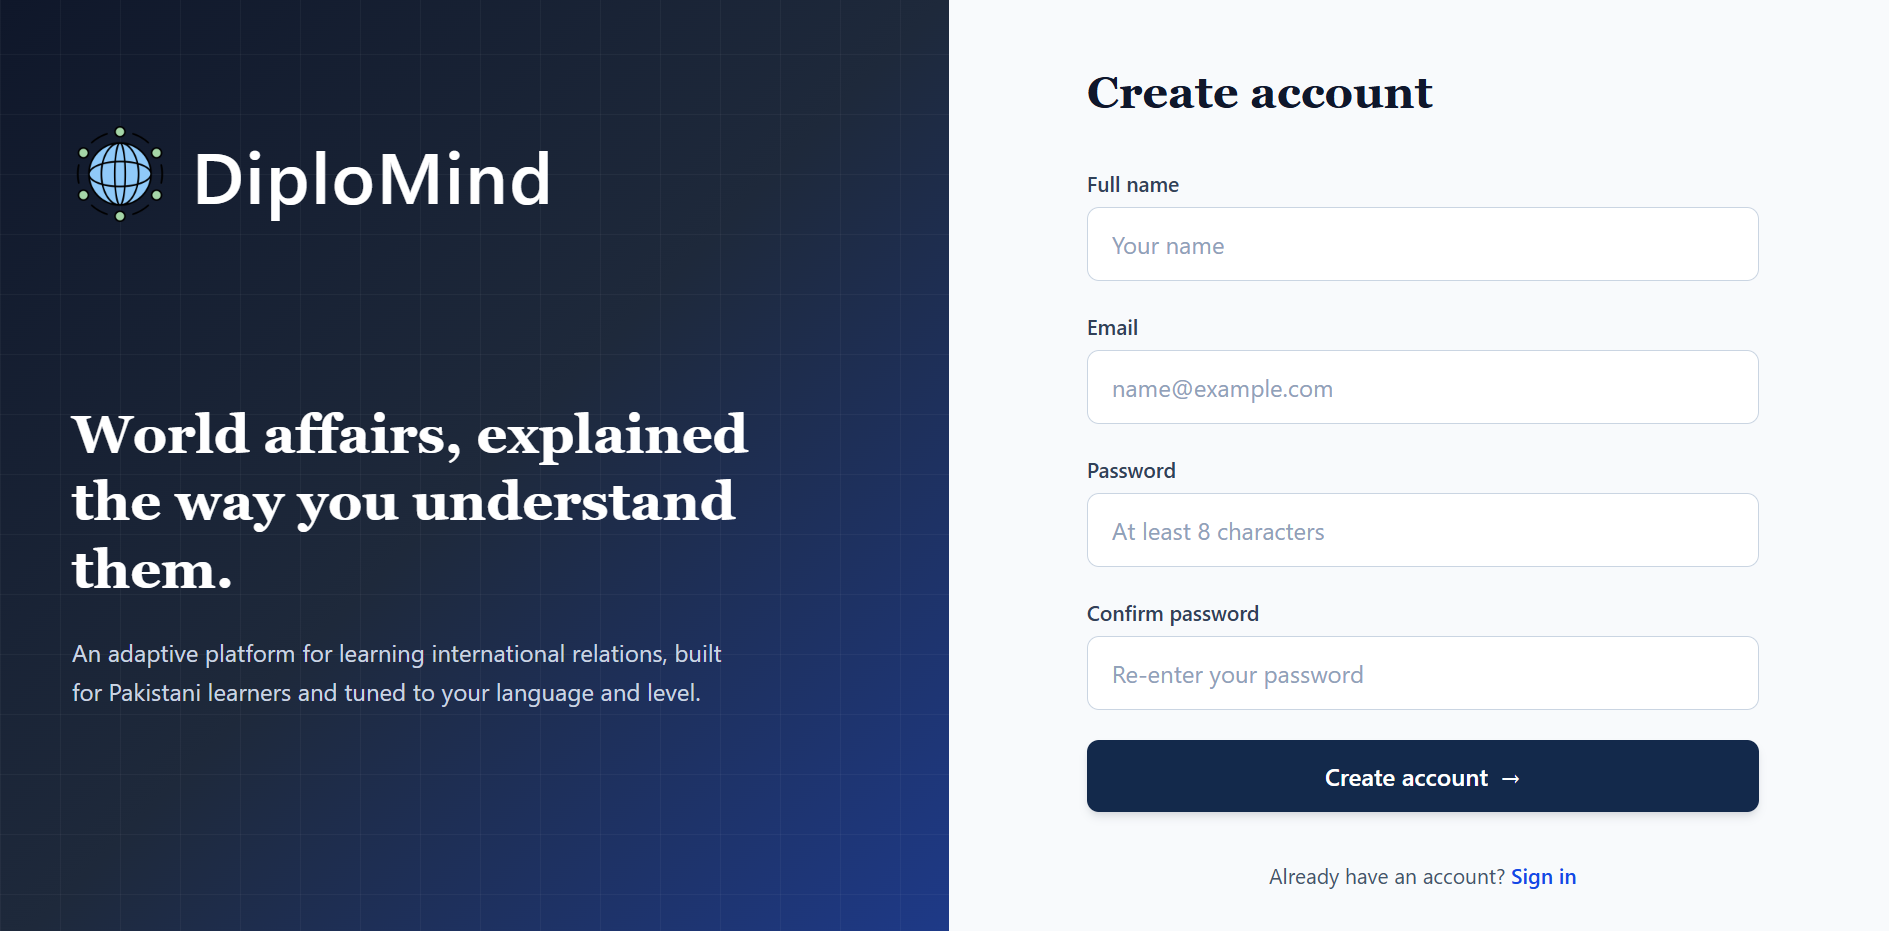
\includegraphics[height=0.31\textheight, keepaspectratio]{Figures/UI_2.png}
    \caption{Sign-Up Screen}
    \label{fig:ui-signup}
    \vspace{2pt}
    \textit{New users can create an account to get started \\(Use Case 1: User Registration).}

\end{figure}

\begin{figure}[H]
    \centering
    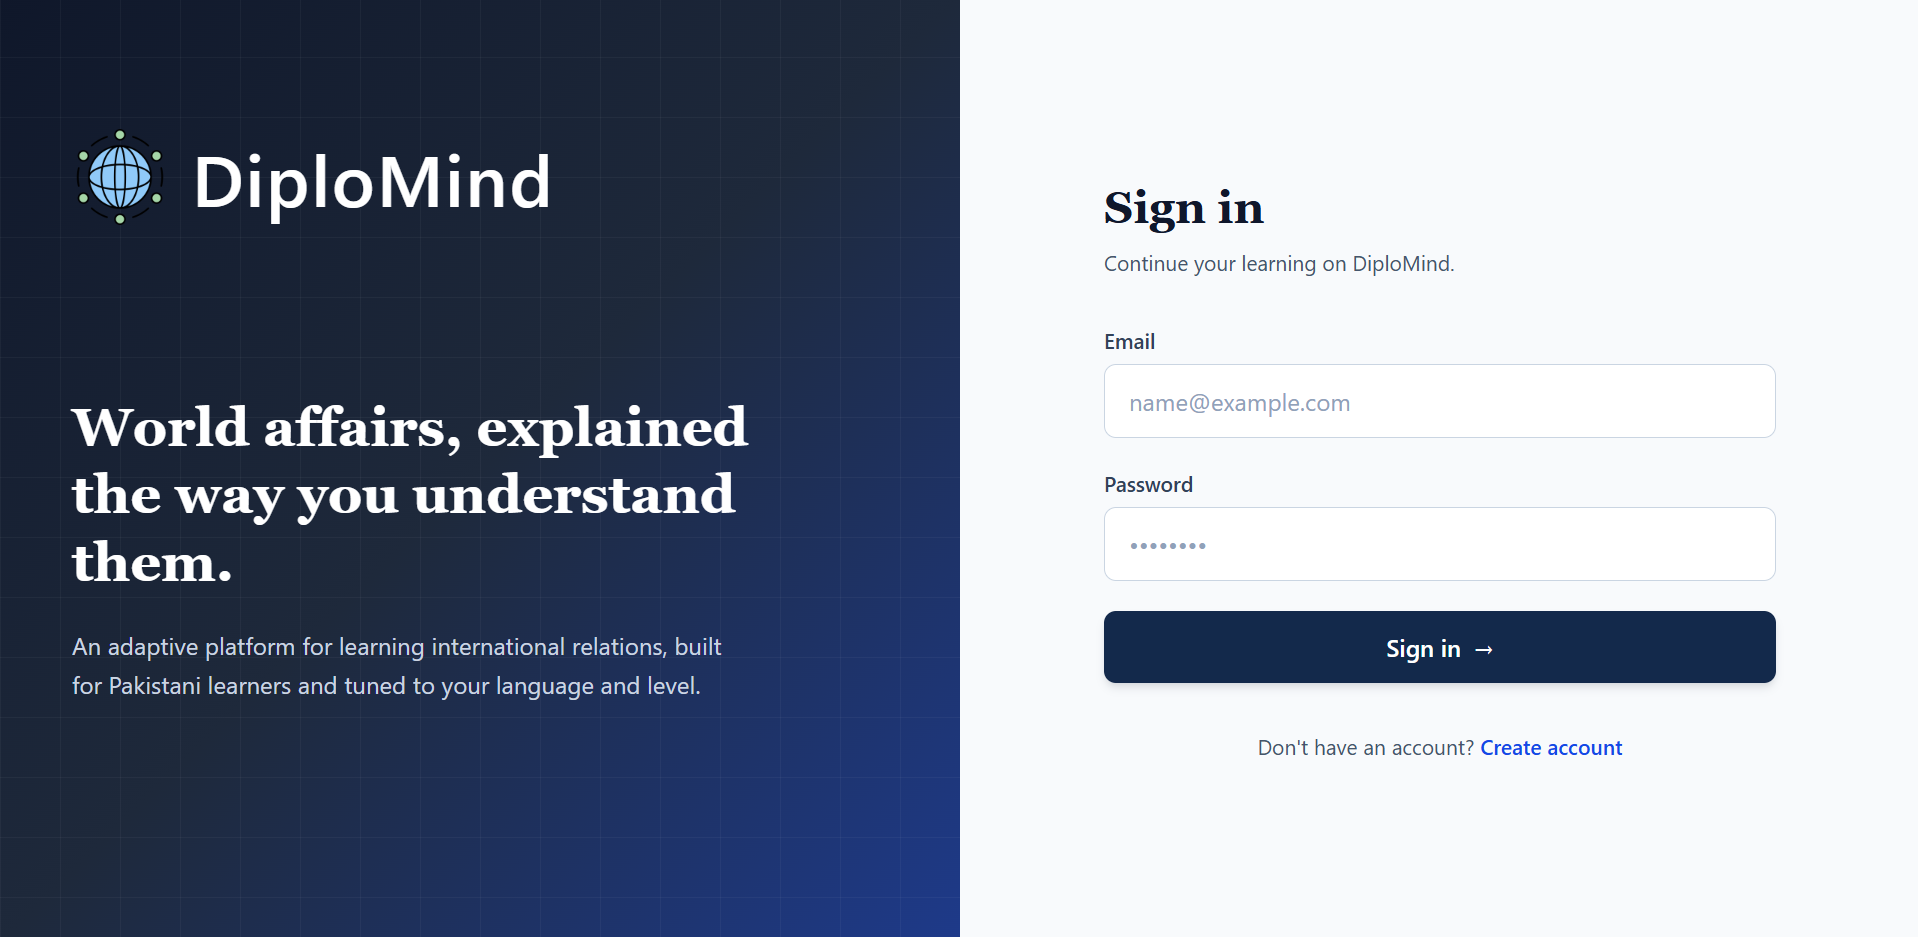
\includegraphics[height=0.31\textheight, keepaspectratio]{Figures/UI_1.png}
    \caption{Sign-In Screen}
    \label{fig:ui-signin}
    \vspace{2pt}
    \textit{Returning users can sign in to continue learning \\(Use Case 2: User Login).}

\end{figure}


\begin{figure}[H]
    \centering
    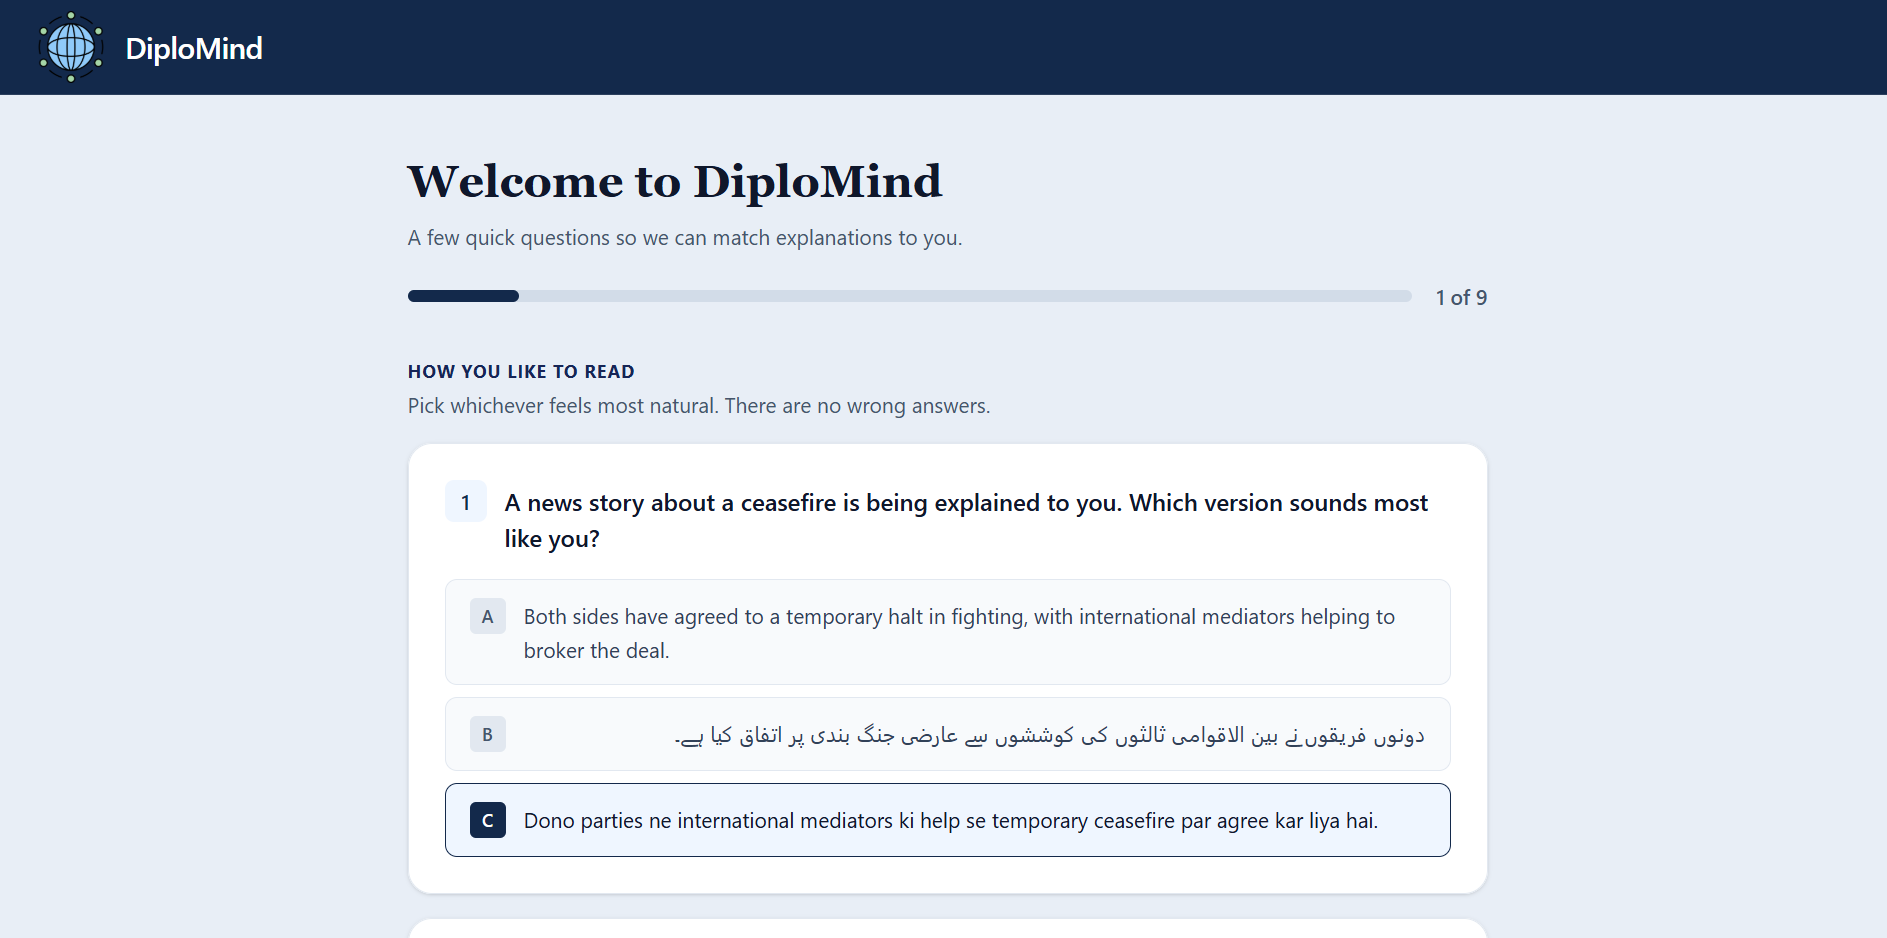
\includegraphics[height=0.31\textheight, keepaspectratio]{Figures/UI_3.png}
    \caption{On-Boarding Quiz Screen No.~1}
    \label{fig:ui-quiz1}
    \vspace{2pt}
    \textit{Users answer short questions so the system can gauge their level \\(Use Case 3: Onboarding Quiz).}

\end{figure}

\begin{figure}[H]
    \centering
    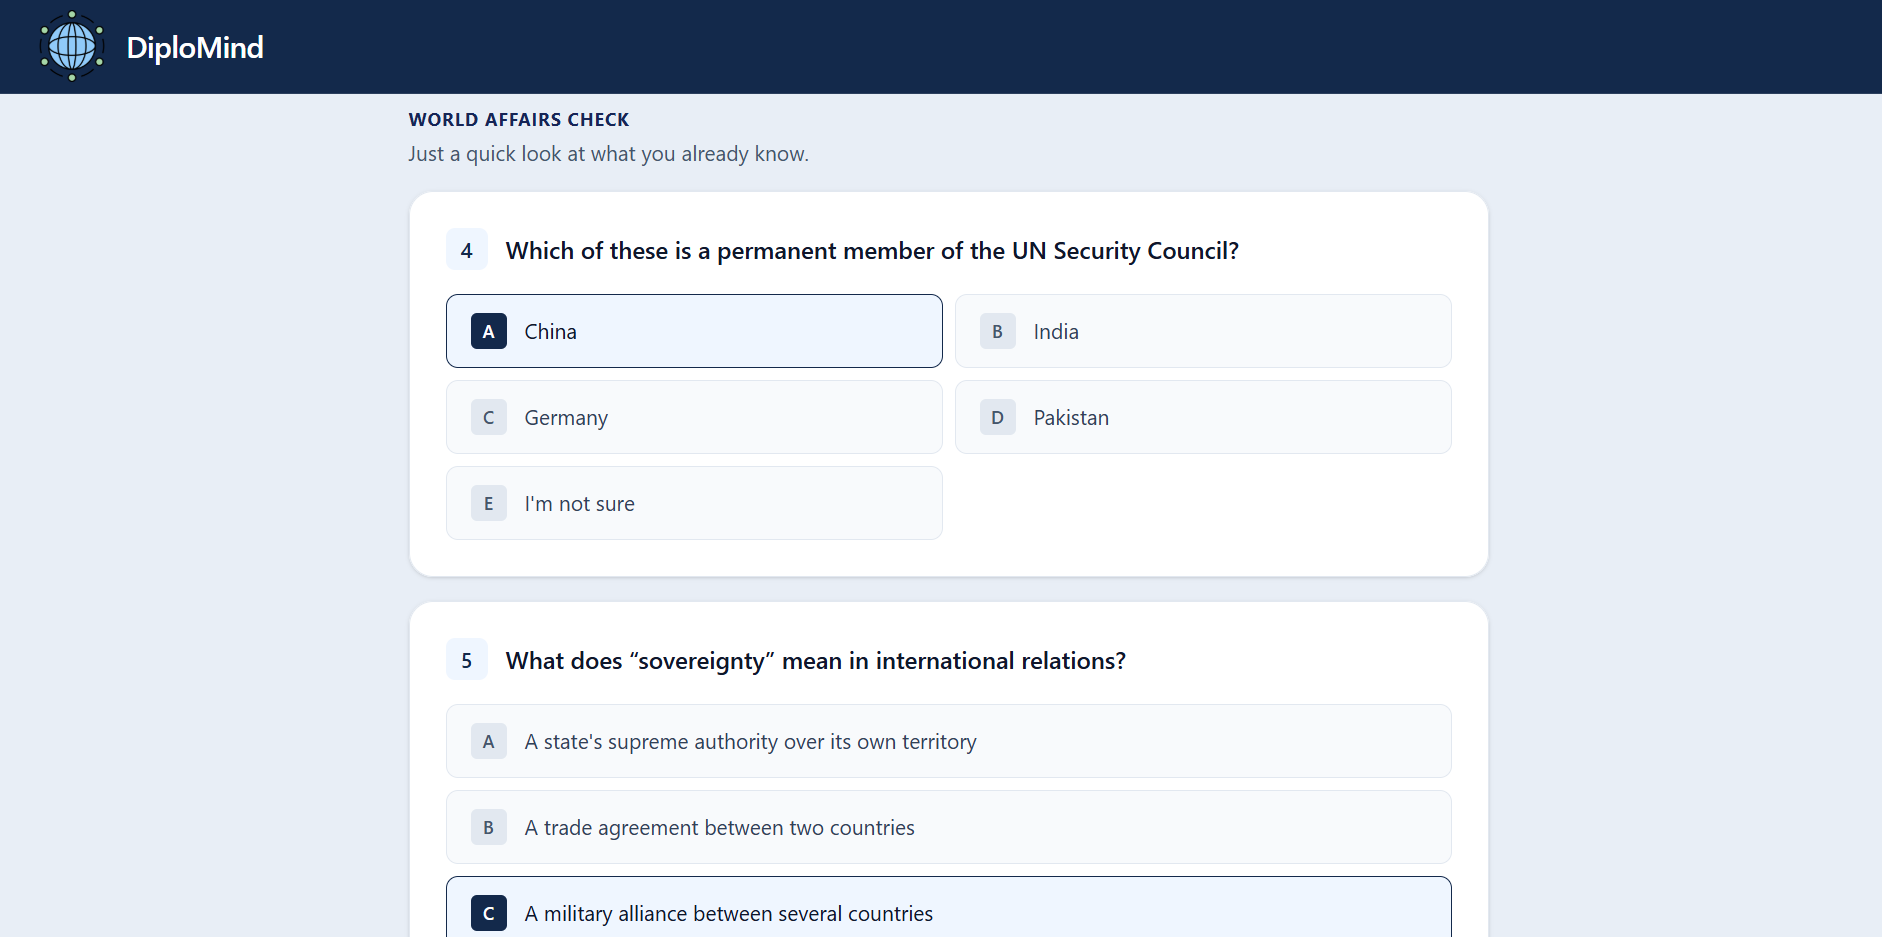
\includegraphics[height=0.31\textheight, keepaspectratio]{Figures/UI_4.png}
    \caption{On-Boarding Quiz Screen No.~2}
    \label{fig:ui-quiz2}
    \vspace{2pt}
    \textit{Users answer short questions so the system can gauge their level \\(Use Case 3: Onboarding Quiz).}

\end{figure}

\begin{figure}[H]
    \centering
    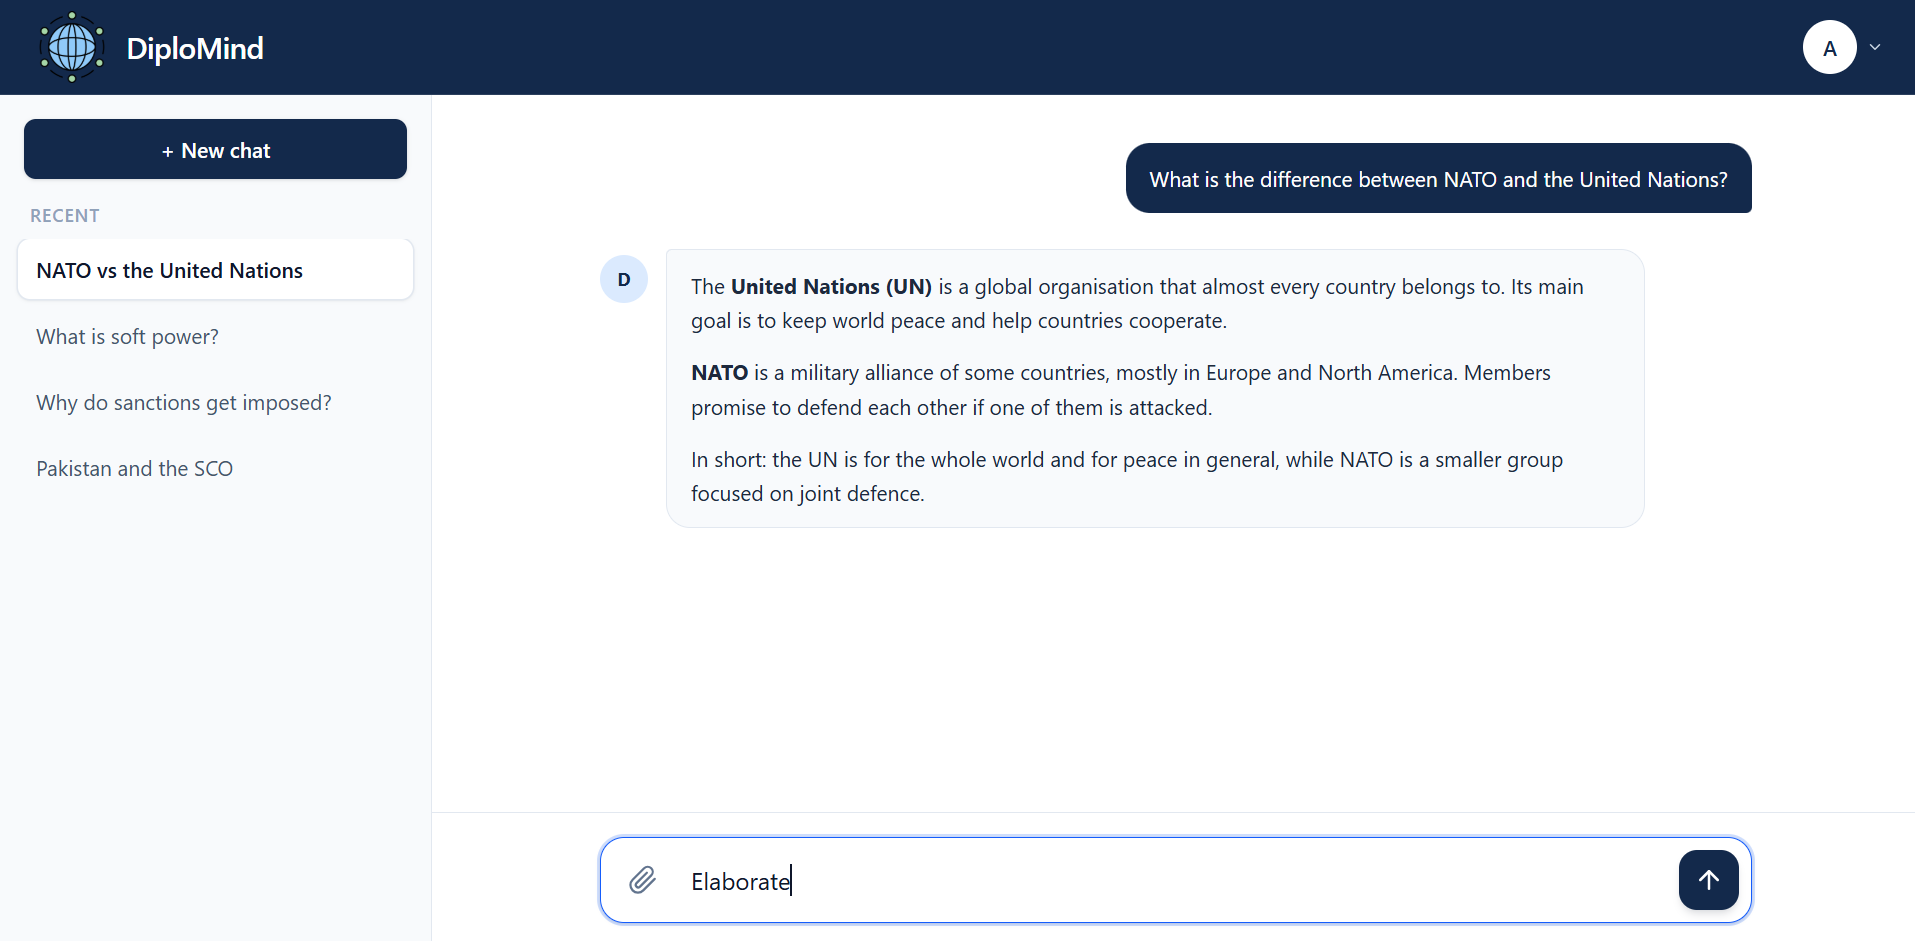
\includegraphics[height=0.31\textheight, keepaspectratio]{Figures/UI_5.png}
    \caption{Chatbot Screen}
    \label{fig:ui-chatbot}
    \vspace{2pt}
    \textit{Users ask questions and get answers matched to their language and level \\(Use Case 4: Ask Question and Receive a Personalized Explanation).}

\begin{figure}[H]
    \centering
    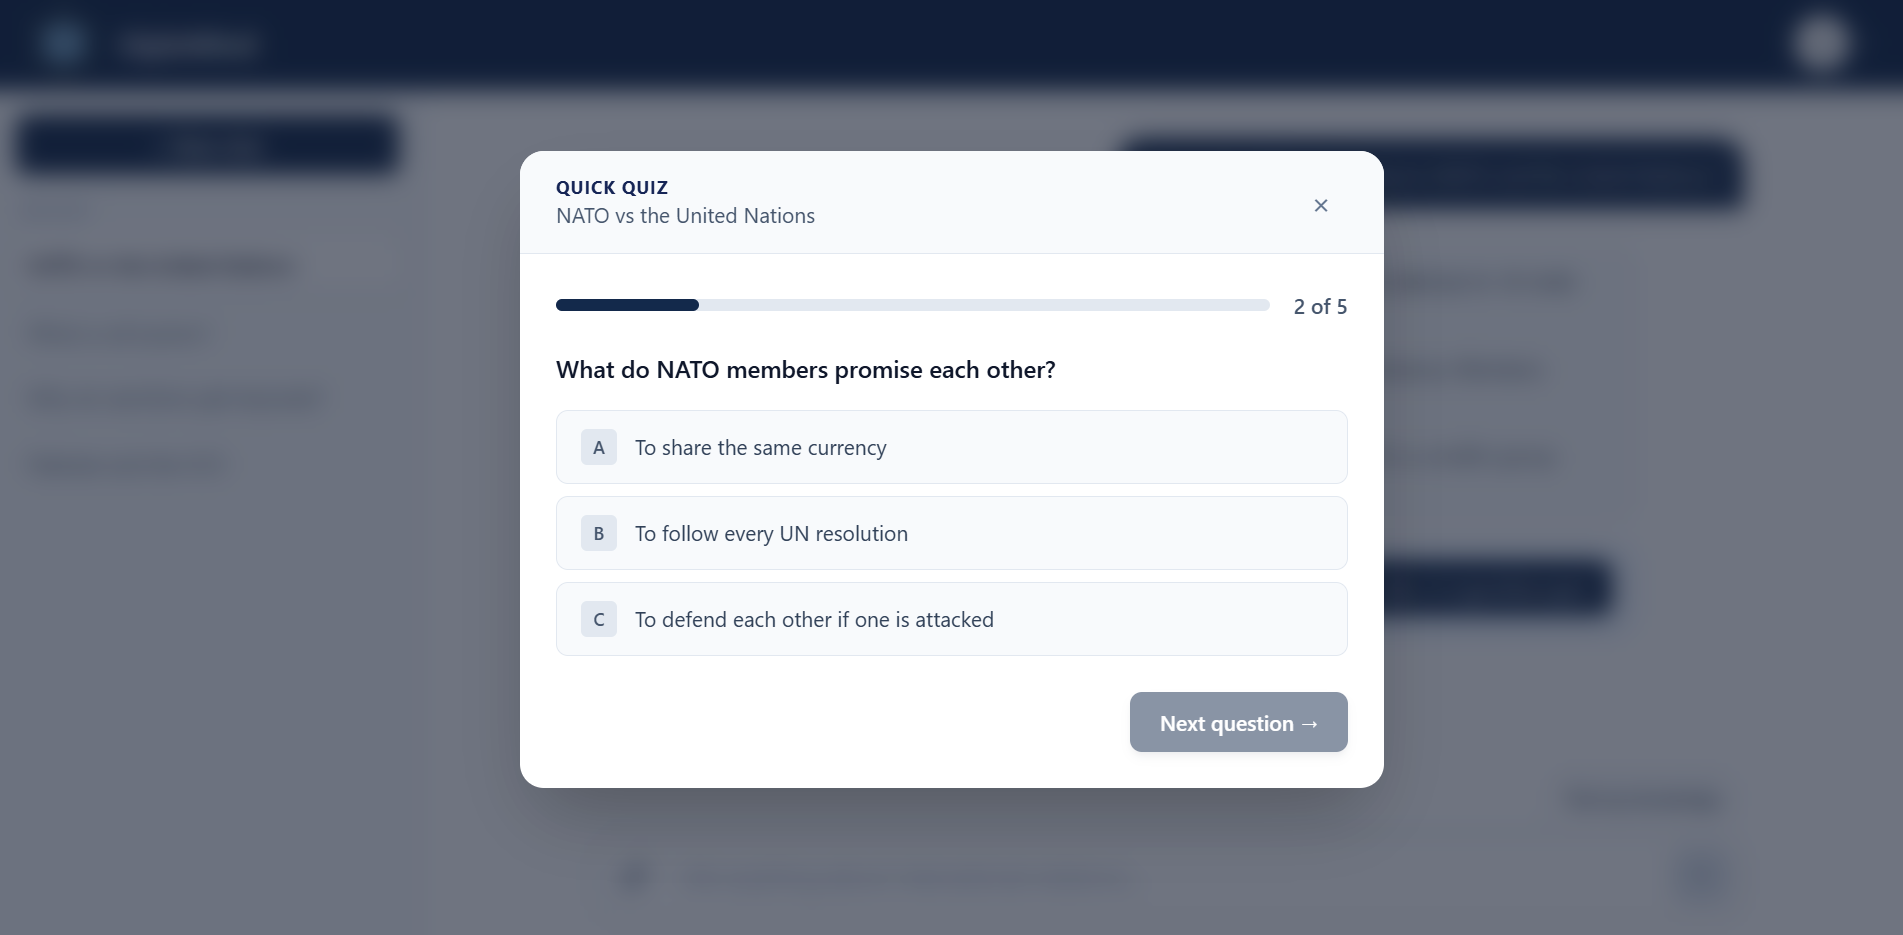
\includegraphics[height=0.31\textheight, keepaspectratio]{Figures/UI_6.png}
    \caption{Post-Explanation Quiz Popup}
    \label{fig:ui-chatquiz}
    \vspace{2pt}
    \textit{After a few questions, a short quiz appears in the chat to check the user's understanding \\(Use Case 5: Take the Post-Explanation Quiz).}
\end{figure}

\end{figure}

\clearpage
\section{Database Design}
DiploMind stores its data in MongoDB, a NoSQL document database. Instead of tables with fixed columns and enforced relationships, the data is kept as collections of flexible, JSON-like documents.  An Entity Relationship Diagram (ERD) is designed for relational databases, where tables are linked through enforced foreign keys, so it does not fit our design. Instead, the data dictionary below describes each collection, its fields, their data types and the collection that each reference field points to. Fields marked (FK) hold the ID of a document in another collection, and the application, not the database, keeps these links consistent.
\subsection{Data Dictionary}

% Needs no extra packages. Column widths assume a standard text width.
\begin{table}[!ht]
\centering
\small
\setlength{\tabcolsep}{4pt}
\caption{Data Dictionary: Article}
\begin{tabular}{|p{2.0cm}|p{2.5cm}|p{1.7cm}|p{1.9cm}|p{1.3cm}|p{4.6cm}|}
\hline
\textbf{Entity} & \textbf{Attribute} & \textbf{Data Type} & \textbf{Relation To} & \textbf{Nullable} & \textbf{Description} \\ \hline
Article & ArticleID & String & & No & Unique ID of the article (PK) \\ \cline{2-6}
 & Source & String & & No & Where the article was scraped from (Dawn, BBC World, ISSI) \\ \cline{2-6}
 & ContentType & String & & No & Either current\_affairs or foundational \\ \cline{2-6}
 & Title & String & & No & Headline of the article \\ \cline{2-6}
 & Link & String & & No & URL of the article page \\ \cline{2-6}
 & PdfUrl & String & & Yes & PDF link, only for PDF-based sources\\ \cline{2-6}
 & ScrapedAt & Date & & No & Date and time the article was scraped \\ \cline{2-6}
 & Text & String & & No & Full extracted text of the article \\ \cline{2-6}
 & PublishedAt & Date & & Yes & Original publication date of the article \\ \cline{2-6}
 & Language & String & & No & Language of the text (en or ur) \\ \hline
\end{tabular}
\end{table}

\begin{table}[!ht]
\centering
\small
\setlength{\tabcolsep}{4pt}
\caption{Data Dictionary: User}
\begin{tabular}{|p{2.0cm}|p{2.5cm}|p{1.7cm}|p{1.9cm}|p{1.3cm}|p{4.6cm}|}
\hline
\textbf{Entity} & \textbf{Attribute} & \textbf{Data Type} & \textbf{Relation To} & \textbf{Nullable} & \textbf{Description} \\ \hline
User & UserID & ObjectId & & No & Unique ID of the user (PK) \\ \cline{2-6}
 & Name & String & & No & Full name of the user \\ \cline{2-6}
 & Email & String & & No & Login email of the user, must be unique \\ \cline{2-6}
 & PasswordHash & String & & No & Hashed password of the user \\ \cline{2-6}
 & Register & String & & No & Preferred language: english, urdu or urdish \\ \cline{2-6}
 & Depth & String & & No & Knowledge level: easy, medium or hard \\ \cline{2-6}
 & Onboarding Completed & Boolean & & No & Whether the onboarding quiz is finished \\ \cline{2-6}
 & CreatedAt & Date & & No & Account creation time \\ \cline{2-6}
 & LastLogin & Date & & Yes & Time of the last login \\ \hline
\end{tabular}
\end{table}

\begin{table}[!ht]
\centering
\small
\setlength{\tabcolsep}{4pt}
\caption{Data Dictionary: Conversation}
\begin{tabular}{|p{2.0cm}|p{2.5cm}|p{1.7cm}|p{1.9cm}|p{1.3cm}|p{4.6cm}|}
\hline
\textbf{Entity} & \textbf{Attribute} & \textbf{Data Type} & \textbf{Relation To} & \textbf{Nullable} & \textbf{Description} \\ \hline
Conversation & ConversationID & ObjectId & & No & Unique ID of the chat session (PK) \\ \cline{2-6}
 & UserID & ObjectId & User & No & Owner of the chat (FK) \\ \cline{2-6}
 & Title & String & & No & Title shown in the chat history sidebar \\ \cline{2-6}
 & CreatedAt & Date & & No & When the chat started \\ \cline{2-6}
 & UpdatedAt & Date & & No & Time of the last message \\ \hline
\end{tabular}
\end{table}

\begin{table}[!ht]
\centering
\small
\setlength{\tabcolsep}{4pt}
\caption{Data Dictionary: Message}
\begin{tabular}{|p{2.0cm}|p{2.5cm}|p{1.7cm}|p{1.9cm}|p{1.3cm}|p{4.6cm}|}
\hline
\textbf{Entity} & \textbf{Attribute} & \textbf{Data Type} & \textbf{Relation To} & \textbf{Nullable} & \textbf{Description} \\ \hline
Message & MessageID & ObjectId & & No & Unique ID of the message (PK) \\ \cline{2-6}
 & ConversationID & ObjectId & Conversation & No & Chat the message belongs to (FK) \\ \cline{2-6}
 & Role & String & & No & Sender of the message: user or assistant \\ \cline{2-6}
 & Content & String & & No & Text of the message \\ \cline{2-6}
 & AdapterPair & Object & & Yes & Language and depth adapter used (assistant messages only) \\ \cline{2-6}
 & SourceArticleIDs & Array of String & Article & Yes & Articles used to answer (FK list) \\ \cline{2-6}
 & CreatedAt & Date & & No & Time the message was sent \\ \hline
\end{tabular}
\end{table}

\begin{table}[!ht]
\centering
\small
\setlength{\tabcolsep}{4pt}
\caption{Data Dictionary: Onboarding Quiz Question Bank}
\begin{tabular}{|p{2.0cm}|p{2.5cm}|p{1.7cm}|p{1.9cm}|p{1.3cm}|p{4.6cm}|}
\hline
\textbf{Entity} & \textbf{Attribute} & \textbf{Data Type} & \textbf{Relation To} & \textbf{Nullable} & \textbf{Description} \\ \hline
Quiz Question & QuestionID & ObjectId & & No & Unique ID of the question (PK) \\ \cline{2-6}
 & Question & String & & No & Question text \\ \cline{2-6}
 & Options & Array of String & & No & Answer choices \\ \cline{2-6}
 & CorrectAnswer & String & & No & The correct option, must be one of Options \\ \cline{2-6}
 & Topic & String & & Yes & IR topic the question covers \\ \cline{2-6}
 & Difficulty & String & & No & easy, medium or hard \\ \cline{2-6}
 & Language & String & & No & Language of the question \\ \hline
\end{tabular}
\end{table}

\begin{table}[!ht]
\centering
\small
\setlength{\tabcolsep}{4pt}
\caption{Data Dictionary: User Onboarding Response}
\begin{tabular}{|p{2.0cm}|p{2.5cm}|p{1.7cm}|p{1.9cm}|p{1.3cm}|p{4.6cm}|}
\hline
\textbf{Entity} & \textbf{Attribute} & \textbf{Data Type} & \textbf{Relation To} & \textbf{Nullable} & \textbf{Description} \\ \hline
Onboarding Response & ResponseID & ObjectId & & No & Unique ID of the response (PK) \\ \cline{2-6}
 & UserID & ObjectId & User & No & User who answered (FK) \\ \cline{2-6}
 & QuestionID & ObjectId & Quiz Question & No & Bank question that was answered (FK) \\ \cline{2-6}
 & SelectedAnswer & String & & No & Option the user picked \\ \cline{2-6}
 & IsCorrect & Boolean & & No & Whether the answer was right \\ \cline{2-6}
 & AnsweredAt & Date & & No & Time the question was answered \\ \hline
\end{tabular}
\end{table}
\clearpage
\begin{table}[!ht]
\centering
\small
\setlength{\tabcolsep}{4pt}
\caption{Data Dictionary: Intermediate Quiz Response}
\begin{tabular}{|p{2.0cm}|p{2.5cm}|p{1.7cm}|p{1.9cm}|p{1.3cm}|p{4.6cm}|}
\hline
\textbf{Entity} & \textbf{Attribute} & \textbf{Data Type} & \textbf{Relation To} & \textbf{Nullable} & \textbf{Description} \\ \hline
Intermediate Quiz Response & ResponseID& ObjectId & & No & Unique ID of the response (PK) \\ \cline{2-6}
 & UserID & ObjectId & User & No & User who answered (FK) \\ \cline{2-6}
 & ConversationID & ObjectId & Conversation & No & Chat the quiz appeared in (FK) \\ \cline{2-6}
 & QuestionText & String & & No & Question generated by the LLM \\ \cline{2-6}
 & Options & Array of String & & No & Answer choices of the generated question \\ \cline{2-6}
 & CorrectAnswer & String & & No & Correct option of the generated question \\ \cline{2-6}
 & SelectedAnswer & String & & No & Option the user picked \\ \cline{2-6}
 & IsCorrect & Boolean & & No & Whether the answer was right \\ \cline{2-6}
 & Reward & Number & & No & Reward value calculated from the answer \\ \cline{2-6}
 & AnsweredAt & Date & & No & Time the question was answered \\ \hline
\end{tabular}
\end{table}

\FloatBarrier
\section{ Risk Analysis}
In this part we highlight some of the risks that are associated with the development, maintenance and scalability of the project.
\subsection{Technical Risks}
DiploMind is built on fast-moving technology such as large language models, LoRA adapters and vector databases, so the tools and models it relies on are likely to change. The base model may need to be replaced by a newer one, which would require the adapters to be trained again, and the libraries and APIs we use may become obsolete and have to be replaced. The scraping pipeline depends on external news websites, so a change in a website's layout can break it. The adapters are trained on LLM-generated and translated Urdu and Urdish text, so mistakes in this data can reach the final answers if it is not reviewed. Updating the model from quiz feedback using the GRPO approach is hard to implement, as it needs a well-designed reward, a lot of compute, and enough user data, so it may have to be replaced by a simpler method. The requirements of the application may also change in the future, thus asking for a product revamp.
\subsection{Business Risks}
Hosting the application, especially running the language model on a GPU server or in the cloud, can be expensive, so the application might need financing. Developers and subject experts may also be needed to maintain the application, keep the knowledge base up to date, and review Urdu and Urdish content. Since the knowledge base comes from news and research websites, their terms of use and copyright rules may limit how the content can be used. The system also stores user profiles and quiz results, so user privacy must be protected, and a data leak would damage trust in the application.

\section{Conclusion}
This chapter defined what DiploMind must do and how well it must do it. It listed the main features of the system and set out its functional, quality, and non-functional requirements, together with the assumptions made. Eight use cases described how a learner registers, completes the onboarding quiz, asks questions, takes comprehension quizzes, changes the explanation language, uploads a document, and requests a web search. The graphical interface screens showed how the main flows will look. The data dictionary defined the data the system stores, and the risk analysis identified the technical and business risks that could affect the project. Together, these requirements form the basis for the methodology and design chapters that follow.


\chapter{Proposed Approach and Methodology}
This chapter describes the methods behind DiploMind. It covers how the data are collected and prepared, how language and depth adapters are trained and combined, how a new learner is placed into a starting group, how the system retrieves evidence and chooses an adapter pair for each request, how learner feedback is turned into a reward, and how the system corrects itself over time.

The central idea is to personalise an explanation along two independent axes: the language it is written in (English, Urdu or Urdish) and its depth (easy, medium or technical). Here Urdish means Urdu-English code-mixed text written in Roman script, the way many Pakistani readers write and speak. The system also keeps improving that personalisation from evidence about whether learners actually understood what they read.

\section{Overview of the Proposed Approach}
The approach has four stages, shown in Figure~\ref{fig:overview}.


\begin{figure}[H]
    \centering
    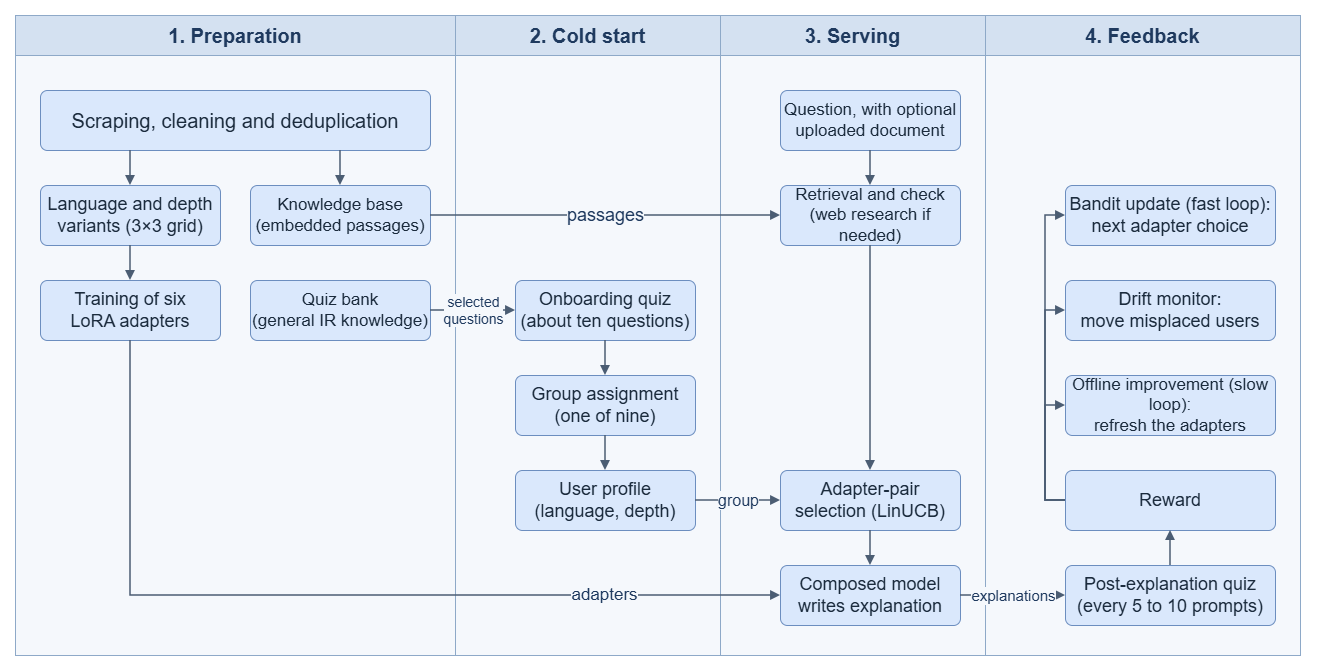
\includegraphics[width=\textwidth, keepaspectratio]{Figures/swimlane.png}
    \caption{Overview of the four stages of the proposed approach}
    \label{fig:overview}
\end{figure}

\begin{enumerate}
  \item \textbf{Offline preparation.} News and international relations (IR) articles are collected and cleaned, a knowledge base is built, and the training data for the language and depth adapters and the quiz bank are prepared.
  \item \textbf{Cold start.} A short onboarding quiz places each new user into one of nine groups (three languages times three depths), which gives a sensible starting point before anything is known about the user.
  \item \textbf{Online serving.} For each question, evidence is retrieved and checked, a bandit selects the adapter pair, the two adapters are combined, and an explanation is generated and formatted. Learners can also upload a document, or ask for web research.
  \item \textbf{Feedback and improvement.} After a short post-explanation quiz, the system turns the learner's result into a reward. This reward is used in three ways. It immediately updates the bandit, so the next adapter choice improves (the fast loop). It helps the drift monitor spot learners who were placed in the wrong group and move them to a better one. It is also saved, so the adapters themselves can be improved later in batches (the slow loop).
\end{enumerate}

Keeping the two loops separate is deliberate. Choosing between existing adapter pairs is cheap and can happen after every quiz, whereas changing the adapters themselves is expensive and needs many results, so it is done in batches.

\section{Data Collection and Dataset Construction}
\subsection{Source Selection and Scraping}
The sources are Pakistani and international news and analysis outlets that publish in English and Urdu, together with foundational explainers on international relations. For every article the scraper stores the title, body text, publication date, URL, outlet and language. We use site-specific scrapers or RSS feeds. Paywalled content is excluded, and article text is used for research only and is not redistributed. So far we have built scraping pipelines and collected articles from the sources in Table~\ref{tab:sources}.

\begin{table}[!ht]
\centering
\caption{Sources used for Data Scrapping}
\label{tab:sources}
\small
\begin{tabular}{|p{3.6cm}|p{3.4cm}|p{6.6cm}|}
\hline
\textbf{Source} & \textbf{Language} & \textbf{Content} \\ \hline
BBC News & English & International and current-affairs news \\ \hline
BBC News Urdu & Urdu & International and current-affairs news in Urdu \\ \hline
Dawn & English & Pakistani newspaper \\ \hline
Express & \textit Urdu & Pakistani newspaper \\ \hline
Geo & \textit Urdu & Pakistani news channel and website \\ \hline
ISSI & English & Analysis from the Institute of Strategic Studies Islamabad \\ \hline
\end{tabular}
\end{table}

\subsection{Cleaning, Filtering and Deduplication}
Raw pages contain much that is not article text, so the collected articles pass through the following steps.

\begin{enumerate}
  \item Boilerplate such as menus, advertisements and related-article lists is removed.
  \item Pages that are not news or analysis are discarded.
  \item A topic filter keeps only international relations and current-affairs content, using a keyword list followed by a classifier.
\end{enumerate}

The publication date is kept throughout, because the knowledge base needs it to prefer recent articles for current-affairs questions.

\subsection{Knowledge Base Construction}
Each cleaned article is split into passages of a few hundred tokens with a small overlap, so that a sentence cut at a boundary still appears whole in one of the passages. Every passage is turned into a vector with a multilingual embedding model and stored in a vector database together with its metadata (outlet, date, language and URL). We plan to compare BGE-M3 and Jina Embeddings v4, among others, as embedding models. Articles stay in their original language, and because the embedding model is multilingual, an English question can retrieve an Urdu passage and the reverse. Multilingual retrieval-augmented generation for knowledge-intensive question answering has been studied by Ranaldi et al. \cite{ranaldi2026multilingual}. New articles are added by a scheduled ingestion job, and older articles can be down-weighted or archived.

\subsection{Building the Language Variants (English, Urdu, Urdish)}
The adapters need aligned examples of the same content in each language. We take Urdu passages and use an LLM with few-shot prompts to produce an English version and an Urdish version of each. This follows the idea of LLM-generated parallel data with human correction, as used to build a Roman Urdu parallel dataset \cite{furqan2024erupd}.

The Urdish prompts are designed around the findings of Winata et al. \cite{winata2026codeswitched}: keeping Urdu grammar as the base and inserting English words where Pakistani speakers naturally use them gave the most natural results. For IR text this mostly means technical and institutional terms such as \emph{sanctions}, \emph{summit} and \emph{veto}. Each prompt contains a few hand-checked examples and an instruction to preserve names, numbers and dates. We write Urdish in Roman script, because Winata et al. found Roman script was usually rated more natural for Urdu-English. Before the generated text is used for training, native speakers review samples of it, and batches that fail the review are regenerated with improved prompts. 

\subsection{Building the Depth Variants (Easy, Medium, Technical)}
Depth is defined by a short rubric (Table~\ref{tab:depth}) so that the three levels can be told apart. For adapter training a few source passages are rewritten at every level by an LLM using the rubric and a few-shot example per level.

\begin{table}[!ht]
\centering
\caption{Rubric for the three depth levels}
\label{tab:depth}
\small
\begin{tabular}{|p{1.9cm}|p{4.3cm}|p{4.5cm}|p{3.1cm}|}
\hline
\textbf{Level} & \textbf{Vocabulary and jargon} & \textbf{Sentences and context} & \textbf{Assumed background} \\ \hline
Easy & Everyday words; jargon avoided or explained in the sentence & Short sentences; a concrete example or analogy & None \\ \hline
Medium & Some standard IR terms, each with a short definition & Moderate length; brief context about the actors and events & Some familiarity with current events \\ \hline
Technical & Field terminology used without explanation & Longer analytic sentences; references to institutions, treaties or theories & Working knowledge of IR \\ \hline
\end{tabular}
\end{table}

\subsection{Training Pairs and Splits}
For every source passage the pipeline produces a grid of nine aligned versions (three languages times three depths), shown in Figure~\ref{fig:grid}. The training pairs are drawn from this grid so that each adapter learns one axis only.

\begin{itemize}
  \item \textbf{Language adapter pairs:} a source passage with a language instruction, paired with the version in that language. The depth of the target is varied evenly across easy, medium and technical, so the adapter does not pick up a hidden depth preference.
  \item \textbf{Depth adapter pairs:} a source passage with a depth instruction, paired with the version at that depth. The language is varied evenly across the three languages.
\end{itemize}

Splits are made by article, not by passage, so that no article appears in both the training and the validation or test data. A fixed set of test passages is held out for the whole project.

\begin{figure}[!ht]
\centering
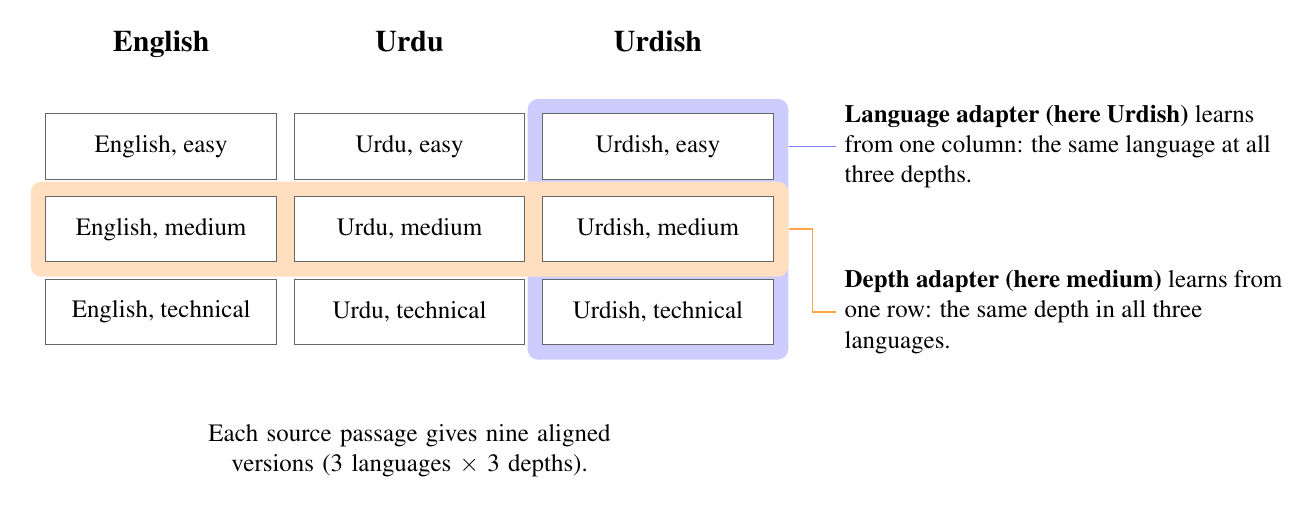
\includegraphics[width=\textwidth]{Figures/fig02_grid.png}
\caption{The 3$\times$3 grid of aligned versions of one source passage, and how the six training sets are drawn from it.}
\label{fig:grid}
\end{figure}


\section{Adapter Training and Composition}
\subsection{Training}
Six adapters are trained: three language adapters and three depth adapters. We use low-rank adaptation (LoRA), which keeps the base language model frozen and trains only small low-rank matrices added to its weights, so each adapter is small and cheap to train and store. Training is supervised fine-tuning with the loss computed on the response tokens only, with the instruction masked. The base model candidates are LLaMA-3-8B and Mistral-7B. Starting settings to tune are a learning rate between $10^{-4}$ and $3\times10^{-4}$, two to four epochs, and early stopping on a validation set.

\subsection{Composition}
For a user in group (language $l$, depth $d$), the model used at inference is the base model plus a weighted sum of the two adapters' low-rank updates:
\begin{equation}
W = W_0 + \lambda_L\,\Delta W_{\mathrm{lang}}(l) + \lambda_D\,\Delta W_{\mathrm{depth}}(d),
\end{equation}
The weights $\lambda_L$ and $\lambda_D$ are chosen on a validation set by grid search. This follows the arithmetic composition of parameter-efficient modules by Zhang et al. \cite{zhang2023composing} and the weighted composition of LoRA modules in LoraHub \cite{huang2024lorahub}, and it is related to the merging of separately trained modules for different preferences in Personalized Soups \cite{jang2023personalized}. Other work selects adapters per query using task embeddings \cite{dhasade2026lorauter}; in contrast, our choice of pair is driven by user feedback.

Composition gives nine behaviours from six adapters, which avoids training nine joint adapters. The two updates may interfere with each other, so the composed model is checked against nine jointly trained adapters as a baseline.



\section{Onboarding Quiz and Group Assignment}
\label{sec:onboarding}
A new user has no history, so the system starts with a short onboarding quiz and uses the answers to place the user in one of the nine groups (three languages times three depths). The placement only needs to be a good starting point, because the drift later corrects users who were placed in the wrong group.

\subsection{Question Design}
The quiz has two parts, one for each axis: language comfort, and background knowledge of international relations. In the language part, the learner tells which style of text they find easiest to read. In the knowledge part, the learner answers questions about common terms (for example \emph{sanctions} or \emph{ceasefire}) and well-known events, in order of increasing difficulty. Every question has an ``I am not sure'' option.

What matters most is that the questions separate the groups. Learners in the same group should give similar answers to a question, and learners in different groups should give clearly different answers on average. A question that everyone answers in the same way tells us nothing about where to place a learner, and a question that learners in the same group answer very differently is too unreliable to be useful. We therefore review the draft questions and replace those that are ambiguous or that nearly everyone answers alike. This idea comes from the cluster-based bandit of Shams et al. \cite{shams2021cluster}, which prefers questions whose answers differ strongly between groups and stay consistent within a group, and we use it here as a guideline for writing and selecting questions. We plan to get these questions reviewed by an IR expert.

\subsection{Scoring and Group Assignment}
The answers are scored with simple fixed rules, one for each axis. For language, the system counts the correct answers in each language and assigns the language in which the learner did best, and a tie is settled by the style the learner said they find easiest. For depth, the share of correct answers in the knowledge part is converted into one of three levels using fixed cut-off points, so that a learner who answers few questions correctly starts at easy and one who answers most of them correctly starts at technical. Skipped questions and ``not sure'' answers count as incorrect.

Combining the two results gives one of the nine groups, which is saved in the user profile and becomes the starting arm for the bandit. If scoring cannot be completed, for example because most questions were skipped, the user is placed in a default group (English, medium depth).

\subsection{Future Work: Adaptive Question Selection}
Building on the idea above, a more advanced version could choose the next question according to how well it separates the groups still in contention, and stop as soon as one group is clearly ahead. This needs the average and spread of answers for every group, which requires pilot data or simulated learners, so we leave it as future work.

\section{Retrieval and Grounded Generation}
\label{sec:retrieval}
Grounding an explanation in retrieved text, as in other retrieval-based tutoring systems \cite{liu2025lpitutor}, keeps it tied to real articles instead of the model's memory. The weakness of this idea is that an explanation is only as good as the passages it is given. If the retrieved passages are off-topic or out of date, the model can still build a fluent but wrong answer on them. We plan to follow the structure of corrective retrieval augmented generation \cite{yan2024corrective}, in which the retrieved evidence is checked before it is used, and the system acts differently depending on how good that evidence is. Figure~\ref{fig:request} shows the three stages: retrieval, knowledge correction and generation. The structure is adapted from the corrective approach of Yan et al. \cite{yan2024corrective}.

\begin{figure}[!ht]
\centering
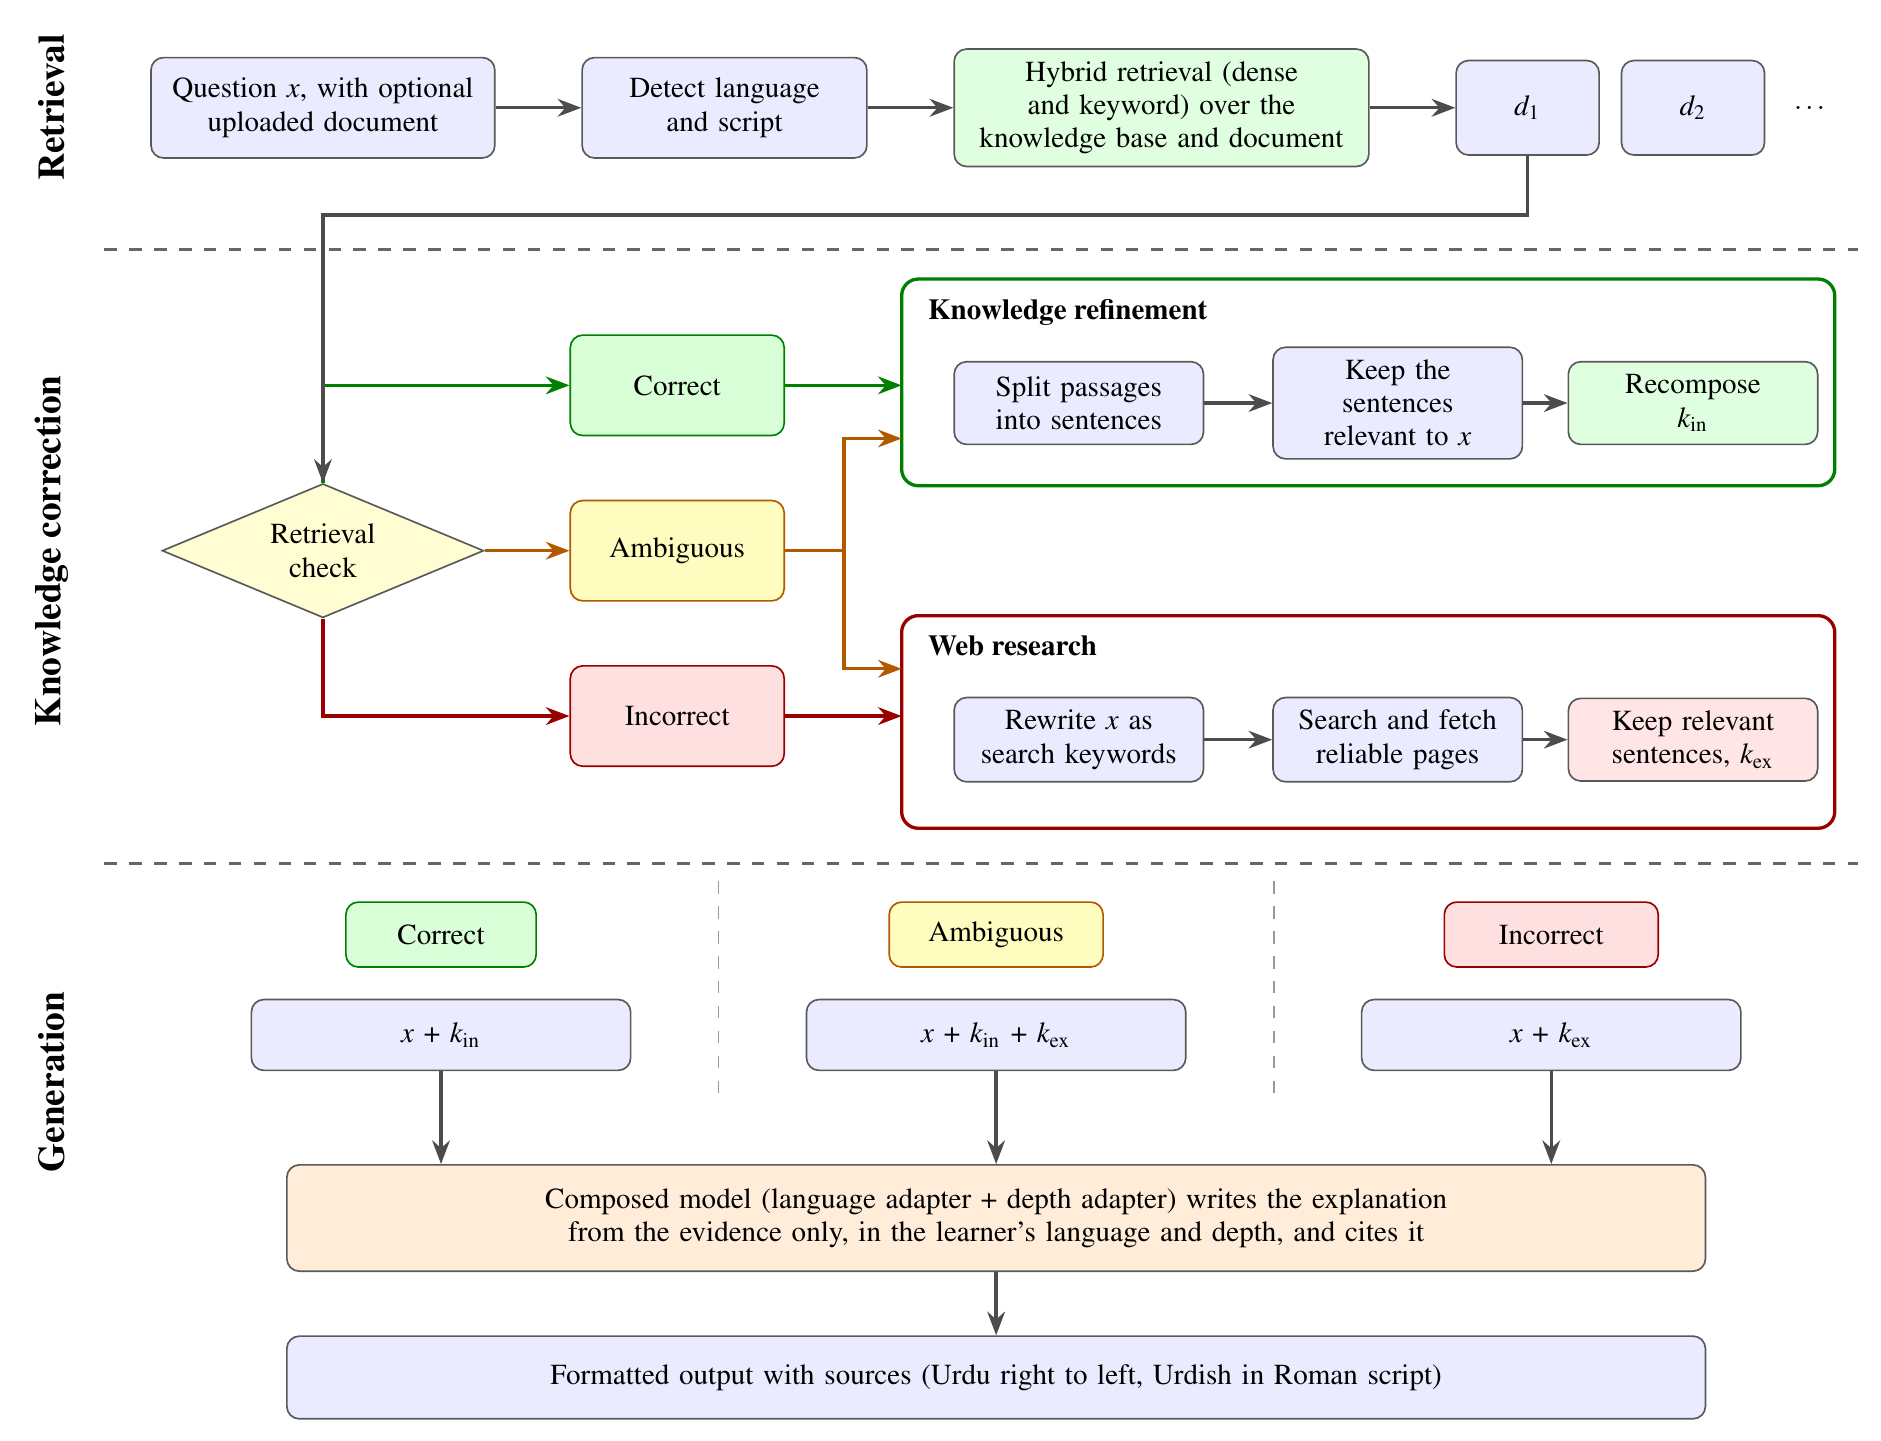
\includegraphics[width=\textwidth]{Figures/fig05_request}
\caption{Processing of one request in DiploMind: retrieval, knowledge correction and grounded generation.}
\label{fig:request}
\end{figure}

\subsection{Retrieval}
When a question arrives, the system first detects its language and script. It then searches the knowledge base. Dense vector search, which matches meaning, is combined with keyword search, which matches exact terms such as names and places, through a weighted score
\begin{equation}
s(p)=\beta\, s_{\mathrm{dense}}(p)+(1-\beta)\, s_{\mathrm{keyword}}(p),
\end{equation}
as in Pxplore \cite{lim2026pxplore}. For current-affairs questions, a recency filter or boost favours newer articles. The best-scoring passages are passed to the next stage.

\subsection{Retrieval Check and Knowledge Correction}
A passage can look similar to a question without actually answering it, so the retrieval is checked before the evidence is used. Yan et al. make this check with a small fine-tuned model. We have no labelled data to train such a model, so we begin with a simpler version based on the retrieval scores and two thresholds. If at least one passage scores above the upper threshold, the retrieval is judged \emph{correct}. If every passage scores below the lower threshold, it is judged \emph{incorrect}. Anything in between is \emph{ambiguous}. The thresholds are tuned on a small set of questions labelled by the team. Each outcome triggers a different action.

\begin{itemize}
  \item \textbf{Correct:} the stored passages are kept and refined.
  \item \textbf{Incorrect:} the stored passages are discarded, and the system turns to web research instead.
  \item \textbf{Ambiguous:} the system does both and combines the results.
\end{itemize}

\textbf{Knowledge refinement.} Even a relevant passage contains sentences that do not help with the question. Each passage is therefore split into sentences, each sentence is scored against the question with the same similarity measure, and only the relevant sentences are kept, in their original order. The result, written $k_{\mathrm{in}}$, is a short and focused piece of evidence.

\textbf{Web research.} When the stored articles cannot answer the question, it is rewritten as a few search keywords, the web is searched, and the top pages are fetched, with reliable outlets preferred. The same sentence-level filtering is then applied, and the result is written $k_{\mathrm{ex}}$.

\subsection{Generation}
The composed model, which combines the language and depth adapters chosen for the user, receives the question together with the evidence that matches the outcome: $k_{\mathrm{in}}$ when retrieval was correct, $k_{\mathrm{in}}$ and $k_{\mathrm{ex}}$ when it was ambiguous, and $k_{\mathrm{ex}}$ when it was incorrect. It is instructed to rely only on this evidence, to write in the learner's language and depth, and to cite its sources. If no usable evidence is found even after web research, the system says that it could not find reliable information instead of guessing. Finally, the output is formatted: Urdu text is displayed right to left, Urdish is shown in Roman script, and the sources are attached.


\section{Adaptive Adapter Selection with LinUCB}
\label{sec:bandit}
The nine language-depth combinations are the arms of a contextual bandit, and the user's group gives the starting arm. A contextual bandit learns which option works best in which situation by trying options and observing the reward, while balancing the use of what looks best against trying alternatives that are less certain. We use the LinUCB approach of Li et al. \cite{li2010contextual}, which scores each arm by its estimated reward given the user's context plus a bonus for arms about which it is uncertain. We apply it as described in that paper and do not repeat its derivation here.

The context describes the user and the request, for example the group, the onboarding scores, the recent average reward, the language of the query and the number of earlier interactions. The final feature list will be fixed during implementation.

Three design choices adapt the bandit to learning:
\begin{itemize}
  \item \textbf{Safe exploration.} The bandit may only choose between the user's current arm and its neighbours, meaning the same language with one depth step up or down, or the same depth with another language. This stops it from showing a technical explanation to an easy-level user as an experiment. The exploration parameter is kept small at first.
  \item \textbf{A warm start.} Each arm starts from the group assigned by the onboarding quiz and not from zero knowledge, and the statistics are shared by users in the same group.
  \item \textbf{One choice per quiz window.} Because the reward arrives only after the post-explanation quiz, the arm is chosen at the start of each window of five to ten prompts and kept for that window, so the reward can be attributed to a single arm.
\end{itemize}

\begin{figure}[!ht]
\centering
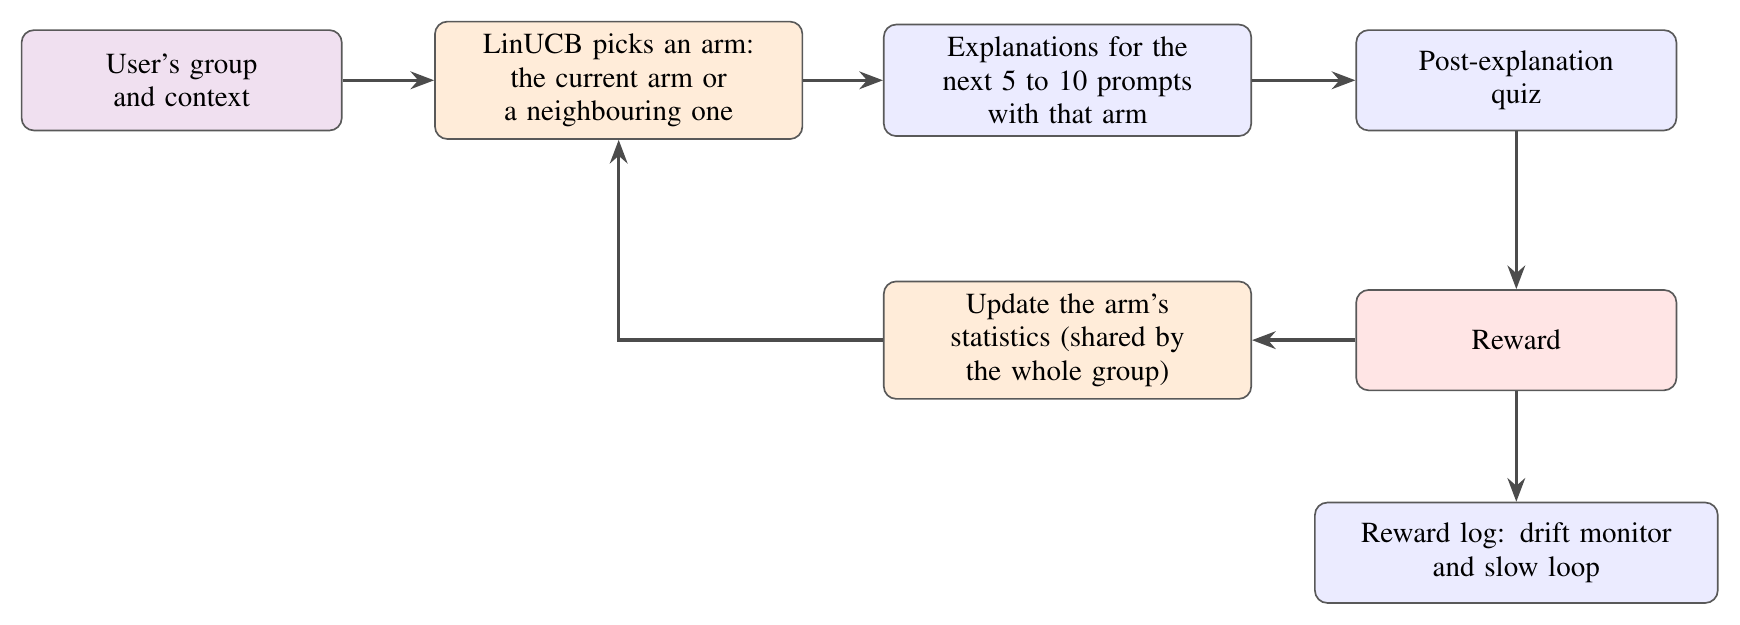
\includegraphics[width=\textwidth]{Figures/fig06_fastloop}
\caption{The fast loop: the bandit chooses an adapter pair, the learner's quiz result becomes a reward, and the reward updates the bandit.}
\label{fig:fastloop}
\end{figure}

\section{Reward Design and the Post-Explanation Quiz}
 
\subsection{Quiz Generation}
After every five to ten prompts from the user, the LLM generates three to five multiple-choice questions from the recent explanations. Along with each question, it gives the correct answer, the sentence from the explanations that supports it, and a difficulty level (easy, medium or hard).  Each question gets a difficulty weight $d_q$ of 1, 2 or 3 based on its level, so that a correct answer to a harder question counts for more.
 
\subsection{Reward}
The reward combines how well the user understood the explanations with how well they matched the requested language and style:
\begin{equation}
    r = \mathrm{clip}\left(w_s s + w_m m - w_p p,\; 0,\; 1\right)
    \label{eq:reward}
\end{equation}
where:
\begin{itemize}
    \item $s = \sum_q d_q c_q \big/ \sum_q d_q$ is the difficulty-weighted quiz score, where $c_q = 1$ if question $q$ is answered correctly and $0$ otherwise;
    \item $m$ is a score from automatic checks of whether the explanation is in the correct language and script and, for Urdish, uses a natural mix of Urdu and English words;
    \item $p$ is a penalty for statements not supported by the sources, the wrong script, or an overly long explanation.
\end{itemize}
The weights $w_s$, $w_m$ and $w_p$ are tuned later. Manual language changes by the user are also logged, since they suggest that the user may be in the wrong group.
 
A quiz score depends not only on the explanation but also on the user's background and on how hard the questions are, so it is a noisy signal. Weighting questions by difficulty and comparing each user's rewards with those of their own group help reduce this noise.

 \section{Drift Detection and Group Reassignment}
\label{sec:drift}
The onboarding quiz can place a user in the wrong group, for example if the user overstated their English, and a user's needs can also change over time. The drift monitor (Figure~\ref{fig:drift}) detects such cases and corrects them by comparing how each user is doing with how the rest of their group is doing.

For every group, the system keeps the mean and standard deviation of the rewards of its users. For every user, it keeps a rolling mean of their last $W$ quiz rewards (for example $W=3$), so that a single bad quiz does not trigger a change. A user is flagged as an outlier if this rolling mean is below the group mean by more than $k$ standard deviations, or if the user repeatedly overrides the assigned language or depth, which is a direct sign that the placement does not suit them.

For a flagged user, the system estimates the expected reward under each neighbouring group, using the bandit's learned model and, if needed, by trying that group for a while. The user is moved only if a neighbouring group's estimate exceeds the current group's by a margin $\delta$, which prevents small or noisy differences from causing a move. After any reassignment, a cool-down period applies so that a user is not moved back and forth, and every event is logged.

The values of $W$, $k$, $\delta$ and the cool-down are tuned in simulation. A similar idea of reviewing a learner against other cohorts and reassigning them appears in Edu-Theater \cite{gao2026edutheater}. A bandit that gradually discounts old data, so that it adapts when preferences change, is a possible extension that we leave to future work.

\begin{figure}[!ht]
\centering
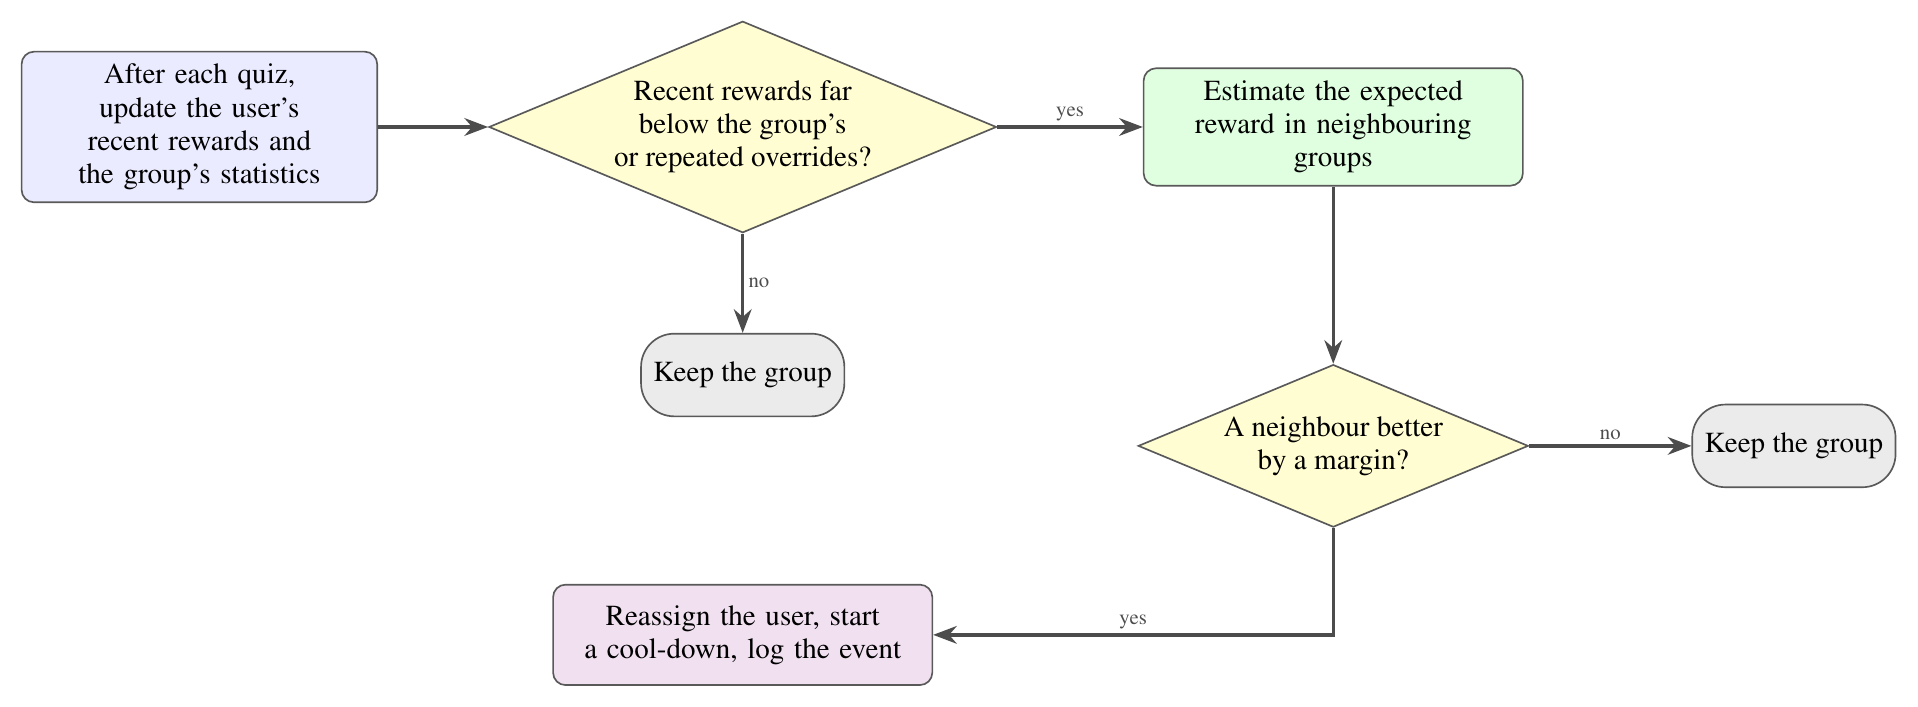
\includegraphics[width=\textwidth]{Figures/fig07_drift}
\caption{Flow of the drift monitor that detects and corrects misplaced users.}
\label{fig:drift}
\end{figure}


\section{Offline Improvement Loop (Slow Loop)}
\label{sec:slowloop}
The slow loop is meant to improve the shared language and depth adapters from accumulated results. A real user sees only one explanation per prompt, so the user's quiz result cannot be used to score other possible explanations of the same prompt. For this reason, the loop works offline. Logged prompts are taken from the system, the current model writes several candidate explanations for each, and the candidates are scored using automatic checks together with an estimate of how well a learner would understand them. This estimate can come from a reward model or from a simulated learner, an LLM that plays a learner of the given group, reads the explanation and answers the quiz, an idea also used to train a tutoring model against simulated students by Dinucu-Jianu et al. \cite{dinucujianu2025teaching}. Because LLM judges can be unreliable in Urdu, any simulated learner has to be checked against real quiz results and native speakers before it is trusted.

The scores are then used to update the six shared adapters, so that every group benefits. The choice on how this update will be done will be made during implementation. We have not yet fixed, and we expect to try the options in order of difficulty. The simplest is to keep the best-scoring candidate for each prompt and train on it with ordinary supervised fine-tuning. A second option is to train on pairs of a better and a worse candidate, so that the better one becomes more likely. The most demanding option is Group Relative Policy Optimization (GRPO) \cite{shao2024deepseekmath}, which compares each candidate with the others written for the same prompt and makes above-average candidates more likely, as Pxplore does after supervised fine-tuning \cite{lim2026pxplore}. We explored GRPO, but it needs several scored candidates per prompt and a reliable reward, so we may switch to the simpler options depending on our time and results.

Whichever option is used, the updated adapters are validated on a held-out test set and on a sample reviewed by native speakers before they replace the current ones, and each new adapter version can be rolled back if it performs worse.

\section{Conclusion}
This chapter presented the methods that make up DiploMind. A data pipeline builds a knowledge base and aligned language and depth variants of news content, and six LoRA adapters are trained and combined by weighted addition. A short onboarding quiz places each learner in one of nine groups, and a contextual bandit tests neighbouring adapter pairs using quiz-based rewards. A drift monitor corrects learners who were placed in the wrong group, and an offline loop improves the shared adapters over time. Explanations are grounded in retrieved evidence, with web research and document upload extending the evidence the system can use. Several choices remain open, notably the base model, the form of the slow-loop optimisation, and the final tuning of the quiz and reward.


\chapter{High-Level and Low-Level Design}
This chapter presents the high-level and low-level design of DiploMind. It starts with a short overview of the system and the design considerations that shaped it, such as our assumptions, constraints and goals. It then presents the system architecture, the architectural strategies we chose, the class diagram and the sequence diagrams, which together show how the system is organized and how its parts work together. Finally, it describes the policies and tactics followed during development.

Together, these sections explain how the system works and how it can be maintained and extended in the future.
\section{System Overview}
DiploMind is a web-based adaptive learning platform that explains international relations (IR) and current-affairs topics to Pakistani readers in the language and depth that suit them. The users of the system are learners, who can create an account, take a short onboarding quiz, ask IR questions in a chat, upload a document to have it explained, ask the system to search the web for a topic, and change their explanation language. Each learner is placed into one of nine groups formed by three languages (English, Urdu and Urdish) and three depth levels, and every explanation is generated from articles in the system's knowledge base and shown with its sources. After every few explanations, a short quiz checks the learner's understanding, and its result is used to keep adjusting the explanations given to that learner.
 
\subsection{DiploMind Modules}
DiploMind achieves personalized and continuously corrected explanations through five modules that work together. The design of each module is discussed in the following subsections.
 
\subsubsection{Data Scraping Module}
This module collects current-affairs and foundational IR content from news and think-tank sources such as Dawn, BBC World and ISSI. The collected articles are cleaned to remove menus, advertisements and other clutter, filtered so that only IR and current-affairs content remains, and tagged by language and content type. Each article is then split into passages, which are embedded with a multilingual embedding model and stored in a vector database, so that a question in one language can retrieve passages in another.
 
\subsubsection{Cold-Start Profiling Module}
This module handles new learners who have no history yet. It presents a short onboarding quiz with questions on language comfort and IR background, where every question offers an ``I am not sure'' option. Based on the answers, the module places the learner into one of the nine language and depth groups, which decides how their first explanations are written.
 
\subsubsection{Content Adaptation Module}
This module produces the explanation for each question. It first retrieves the most relevant passages from the knowledge base, re-ranks them and checks whether they are relevant enough to be used. A LinUCB contextual bandit then selects a language adapter and a depth adapter for the learner, and the two LoRA adapters are combined on a shared base language model to generate an explanation that uses only the retrieved passages and cites them. The same module explains uploaded documents and web search results when the learner requests them.
 
\subsubsection{Feedback and Reward Module}
This module checks whether the explanations were actually understood. After every 5--10 questions, it generates a short multiple-choice quiz from the recent explanations and scores the learner's answers. The score is used as a reward for the adapter pair that produced the explanations, updating the bandit immediately, and it is stored so that the shared adapters can be improved periodically.
 
\subsubsection{Drift Detection Module}
This module checks whether a learner's group is still correct over time. It compares the learner's recent quiz rewards with the average rewards of their group, and flags learners who perform much worse than their group or who repeatedly change the assigned language. A flagged learner is moved to a neighbouring group if that group is expected to suit them better, with a cool-down period after each move so that the learner is not switched back and forth.
 

\section{Design Considerations}
This section addresses the critical aspects that shape the foundation of the design process for DiploMind.
 
\subsection{Assumptions and Dependencies}
This section describes the assumptions and dependencies that shape the design and functionality of DiploMind.
 
\subsubsection{Assumptions}
\begin{itemize}
    \item Learners have a modern web browser and an internet connection.
    \item Learners can read at least one of the three languages offered: English, Urdu or Urdish.
    \item The information given by learners during onboarding may not be accurate, which is why drift detection is part of the design.
    \item The selected news and think-tank sources remain publicly accessible and allow their content to be used for research.
    \item Separately trained language and depth adapters can be combined without one cancelling the effect of the other.
    \item A learner's quiz score reflects how well they understood the explanations they received, so it can be used as a reward.
    \item The group statistics needed for the onboarding quiz can be obtained from a pilot study, expert estimates or simulated learners, since the system starts without users.
\end{itemize}
 
\subsubsection{Dependencies}
\begin{itemize}
    \item The system depends on an open instruction-tuned base language model, such as Llama-3-8B or Mistral-7B, and on PyTorch, Hugging Face Transformers and PEFT to train and combine its adapters. Replacing the base model requires the adapters to be trained again.
    \item Retrieval depends on a multilingual embedding model, such as BGE-M3 or Jina Embeddings v4, and on a vector database to store and search the passages.
    \item The knowledge base depends on the scraping pipeline and on the structure of the source websites. A change in a website's layout can break its scraper.
    \item The web search feature depends on an external search service and an internet connection.
    \item Explaining scanned documents depends on Tesseract OCR with Urdu language support.
    \item The quality of the Urdu and Urdish training data depends on review by native speakers.
    \item Training the adapters and running the model depend on the availability of a GPU with at least 16 GB of memory.
\end{itemize}
 
\subsection{General Constraints}
The design of DiploMind is shaped by the following constraints, each of which has a significant effect on the system.
 
\subsubsection{Hardware Constraints}
The system is not hosted on a server and runs on a single GPU with about 16 GB of memory, either on a local machine or on Kaggle. This limits the size of the base model and the number of learners that can be served at the same time, and is one of the main reasons for using small adapters on a single shared model instead of a separate model for each group.
 
\subsubsection{Data Availability}
There is no existing dataset of IR content written in English, Urdu and Urdish at different depths. The training data for the adapters therefore has to be generated with a language model and then reviewed by native speakers, which takes time and limits the size of the dataset. Urdish also has no standard spelling, which makes its quality harder to check.
 
\subsubsection{Source Availability}
The knowledge base relies on scraping external websites, which can change their layout or restrict access at any time. Their terms of use also limit how the content can be used, so paywalled content is excluded and scraped articles are used for research only.
 
\subsubsection{Performance Requirements}
The system should generate an explanation within about 20 seconds and respond to other actions, such as login and loading chats, within 2 seconds. These limits affect how many passages can be re-ranked and how long the generated explanations can be.
 
\subsubsection{Security and Privacy}
Passwords must be stored as salted hashes, each learner must be able to access only their own data, and uploaded documents must be deleted after the session and never added to the shared knowledge base.
 
\subsubsection{Language and Script}
Urdu must be displayed right-to-left, Urdish in Roman script and English left-to-right. Extracting text from scanned Urdu documents is also difficult, which limits the quality of explanations for such documents.
 
\subsection{Goals and Guidelines}
The goals and guidelines followed in the design and development of DiploMind are discussed below.
 
\subsubsection{Simplicity}
Following the KISS principle (``Keep it simple, stupid!''), each component starts with the simplest method that can work and is made more complex only if needed. For example, a fixed-rule scoring of the onboarding quiz is kept as an alternative to the adaptive quiz, and the adapters are first improved with the simplest training option before more advanced methods are tried.
 
\subsubsection{Grounded and Reliable Answers}
Since IR content is political and changes quickly, an explanation that is easy to read but not supported by a source is not acceptable. Every explanation is therefore based on retrieved sources and shows them, and the learner is told when no relevant source is found.
 
\subsubsection{Safe Personalization}
The system should never show a learner an explanation far from their level just to experiment. The bandit is only allowed to try neighbouring adapter pairs, and a learner who is moved to another group cannot be moved again until a cool-down period has passed.
 
\subsubsection{Modularity}
The base model, adapters, retriever, databases and bandit are designed as separate modules, so that any one of them can be replaced or extended without changing the others. This matters because the technologies used in the project change quickly.
 
\subsubsection{User-Centric Design}
The interface is designed to feel like the chat assistants that learners already use, so that it is familiar and needs no instructions. Computationally expensive work, such as scraping new articles and improving the adapters, runs in the background so that it does not slow down the learner.

 %\begin{comment}
\subsection{Development Methods}
The software design and development of DiploMind follows an agile and iterative approach. The project is divided into a research phase and a development phase, and during development the system is built in small increments, starting with the scraping pipeline and the adapters and then adding retrieval, onboarding, the feedback loop and drift detection. The waterfall model was considered, but it was not selected because the research parts of the project, such as how well the adapters combine and how the reward should be designed, have uncertain outcomes that may require earlier decisions to be revisited.
%\end{comment}

 
\section{System Architecture}
This section outlines the architecture of DiploMind through diagrammatic representations. It gives a high-level overview of the system and describes how its responsibilities are divided among subsystems. The architecture of DiploMind consists of two main parts: the offline preparation part and the online learning part. The offline preparation part collects and processes articles to build the knowledge base, and prepares the data used to train the language and depth adapters. The online learning part serves the learner through the web interface: it places a new learner into a group, retrieves evidence and generates a personalized explanation for each question, and uses quiz results to update the adapter selection and detect misplaced learners. The web interface communicates with the backend through API requests, and the backend stores its data in a NoSQL database and a vector database. The high-level architecture of the system is shown in Figure~\ref{fig:architecture}.
 
\begin{figure}[H]
    \centering
    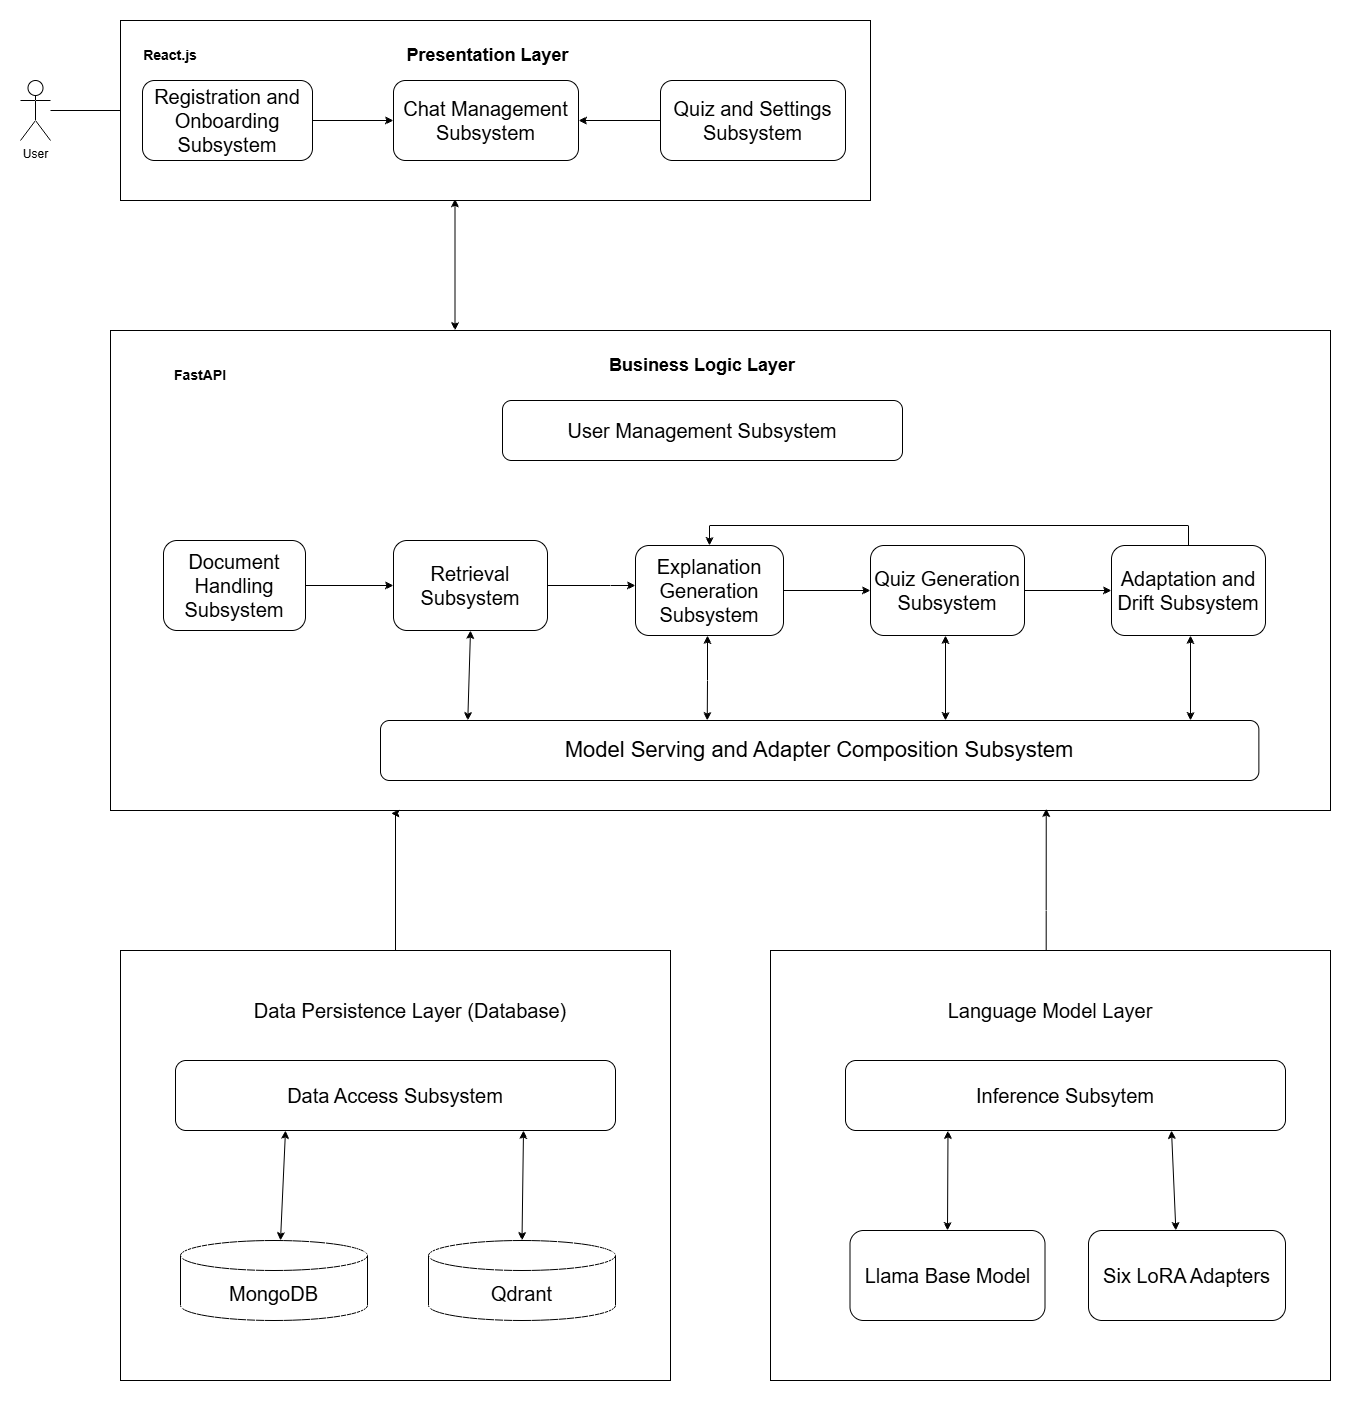
\includegraphics[width=\textwidth, height=0.75\textheight, keepaspectratio]{Figures/diplomind-architecture.png}
    \caption{High-level Architecture Diagram}
    \label{fig:architecture}
    \vspace{2pt}
    \textit{This is the high-level architecture diagram of DiploMind.}
\end{figure}
 
\subsection{Data Scraping and Knowledge Base}
The Data Scraping subsystem acquires the content used to answer learners' questions. It consists of three components: the scraper, the preprocessor and the indexer. The scraper uses site-specific scrapers and RSS feeds to fetch articles, storing the title, text, publication date, link, source and language of each article. The preprocessor removes boilerplate content, checks the language, filters out content that is not related to IR or current affairs, and tags each article as current affairs or foundational. The indexer splits each article into passages, embeds them with the multilingual embedding model and stores them in the vector database, while the full article is stored in the NoSQL database. The structure of this subsystem is shown in Figure~\ref{fig:arch-scraping}.
 
\begin{figure}[H]
    \centering
    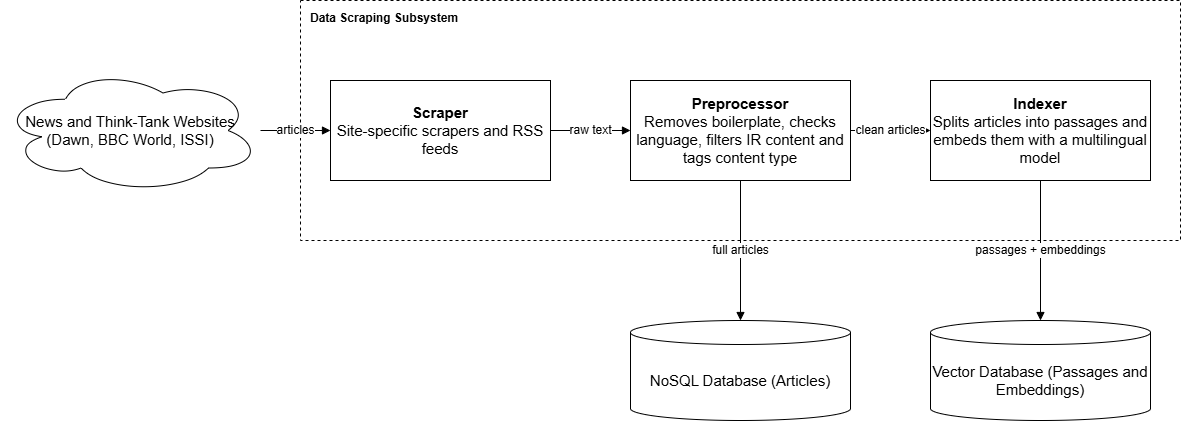
\includegraphics[width=\textwidth, height=0.45\textheight, keepaspectratio]{Figures/arch_scraping.png}
    \caption{Data Scraping - Subsystem Architecture Diagram}
    \label{fig:arch-scraping}
    \vspace{2pt}
    \textit{This figure represents the Data Scraping and Knowledge Base subsystem.}
\end{figure}
 
\subsection{Cold-Start Profiling}
The Cold-Start Profiling subsystem consists of the question selector, the answer recorder and the group assigner. The question selector picks onboarding questions from the question bank, asking first the questions that best separate the groups. The answer recorder saves each answer as soon as it is given, so that an interrupted quiz can be resumed. The group assigner updates the score of each group after every answer and, once one group clearly leads or about ten questions have been asked, stores the learner's language and depth in their profile. The structure of this subsystem is shown in Figure~\ref{fig:arch-profiling}.
 
\begin{figure}[H]
    \centering
    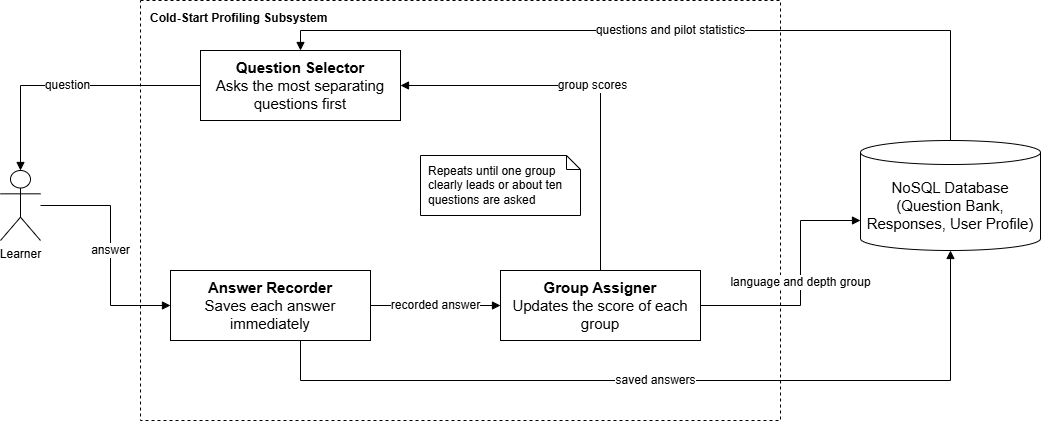
\includegraphics[width=\textwidth, height=0.45\textheight, keepaspectratio]{Figures/arch_profiling.png}
    \caption{Cold-Start Profiling - Subsystem Architecture Diagram}
    \label{fig:arch-profiling}
    \vspace{2pt}
    \textit{This figure represents the Cold-Start Profiling subsystem.}
\end{figure}
 
\subsection{Content Adaptation}
The Content Adaptation subsystem has four major components: the retriever, the adapter selector, the generator and the formatter. The retriever searches the vector database for passages related to the question, re-ranks them with the language model and keeps only the relevant ones; when the learner enables web search or uploads a document, the web pages or the document text are used as the evidence instead. The adapter selector uses the LinUCB bandit to choose a language adapter and a depth adapter for the learner. The generator combines the two selected adapters with the base model and generates an explanation that uses only the evidence and cites it. Finally, the formatter displays the explanation in the correct script and direction and attaches the source links. The structure of this subsystem is shown in Figure~\ref{fig:arch-adaptation}.
 
\begin{figure}[H]
    \centering
    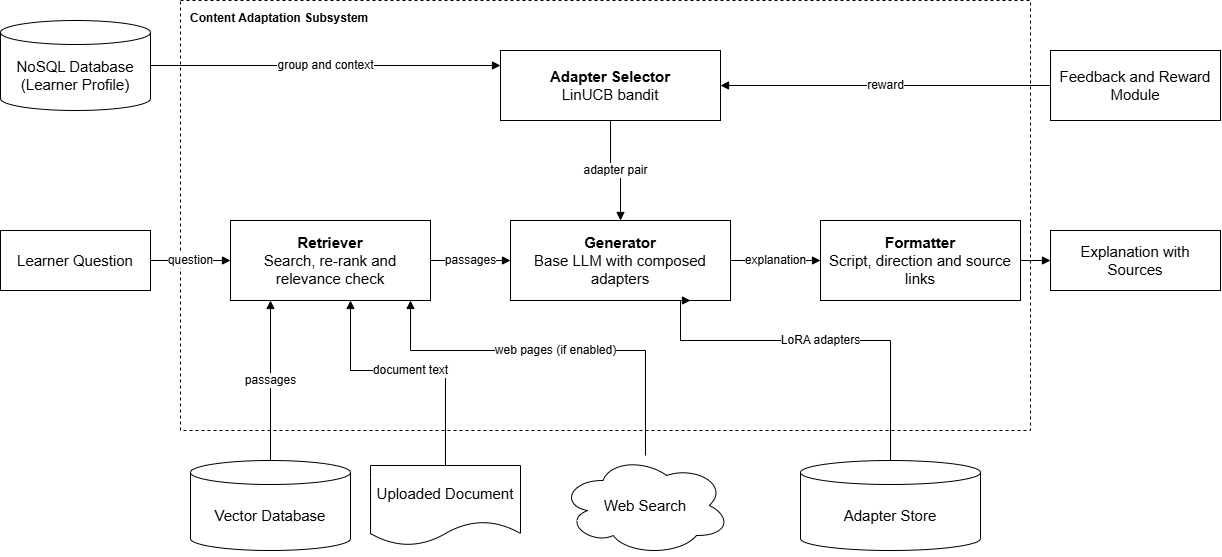
\includegraphics[width=\textwidth, height=0.45\textheight, keepaspectratio]{Figures/arch_adaptation.png}
    \caption{Content Adaptation - Subsystem Architecture Diagram}
    \label{fig:arch-adaptation}
    \vspace{2pt}
    \textit{This figure represents the Content Adaptation subsystem.}
\end{figure}
 
\subsection{Feedback and Drift Detection}
The Feedback and Drift Detection subsystem consists of the quiz generator, the reward calculator and the drift monitor. The quiz generator creates multiple-choice questions from the learner's recent explanations and discards questions whose answers are not supported by them. The reward calculator scores the learner's answers, uses the score to update the bandit for the adapter pair that was used, and stores the result in the database. The drift monitor compares the learner's recent rewards with the rewards of their group and moves the learner to a better-suited neighbouring group when needed. The stored results are also used periodically to improve the shared adapters. The structure of this subsystem is shown in Figure~\ref{fig:arch-feedback}.
 
\begin{figure}[H]
    \centering
    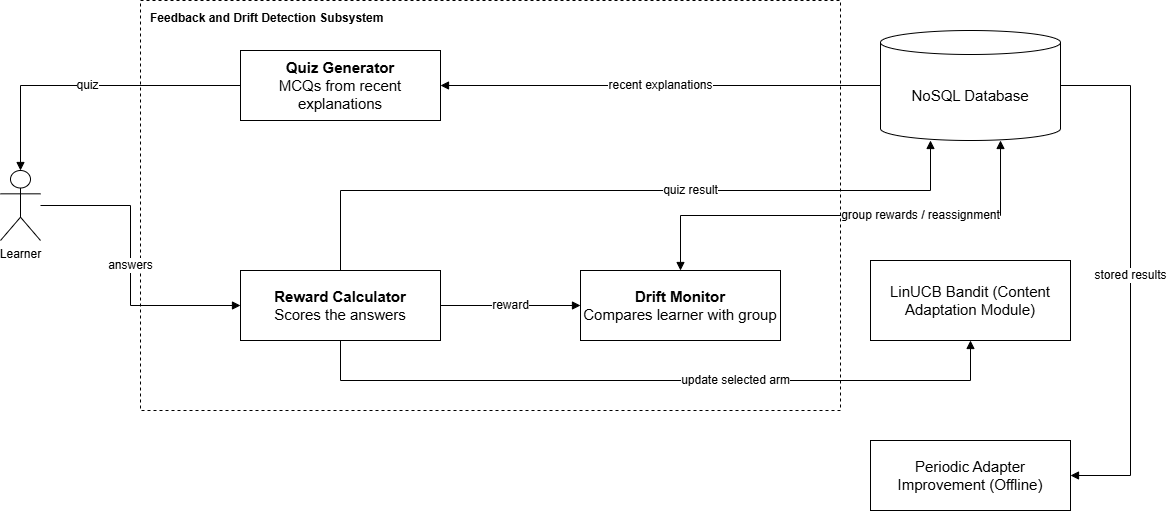
\includegraphics[width=\textwidth, height=0.45\textheight, keepaspectratio]{Figures/arch_feedback.png}
    \caption{Feedback and Drift Detection - Subsystem Architecture Diagram}
    \label{fig:arch-feedback}
    \vspace{2pt}
    \textit{This figure represents the Feedback and Drift Detection subsystem.}
\end{figure}



\section{Architectural Strategies}
The architectural strategies that we will be using for DiploMind are given below.
 
\subsection{Tools and Software}
The backend of DiploMind will be developed in Python using FastAPI. The language and depth adapters will be trained and combined using PyTorch, Hugging Face Transformers and PEFT on an open base model such as Llama-3-8B or Mistral-7B, with training carried out in Jupyter and Kaggle notebooks. For retrieval, a multilingual embedding model such as BGE-M3 or Jina Embeddings v4 will be used with a vector database and BM25 keyword search. Requests, BeautifulSoup and RSS feed parsers will be used to build the scrapers, and Tesseract OCR will be used to extract text from scanned documents. Git and GitHub will be used for version control and Draw.io for the design diagrams. Using Python across the backend, scraping and machine learning allows all parts of the system to be integrated easily.
 
\subsection{Client-Server Model}
The project adopts a client-server model in which the web interface communicates with the backend through API requests. The backend handles sessions, retrieval, adapter selection and generation, so the interface only sends the learner's input and displays the result. This separation also allows another front end, such as a mobile application, to use the same backend in the future.
 
\subsection{Database}
A NoSQL database such as MongoDB will be used to store users, conversations, messages, articles, the onboarding question bank and quiz responses, since these records are nested and their fields may change during development. The passages of the knowledge base and their embeddings will be stored separately in a vector database, which is designed for fast similarity search. The reasons for choosing a NoSQL database are discussed further in Section~6.7.2.
 
\subsection{Adapter-Based Personalization}
Instead of training a separate model for each of the nine groups, DiploMind uses one shared base model with six small LoRA adapters: three for language and three for depth. For each request, the selected language adapter and depth adapter are combined with the base model by weighted addition, which produces nine different behaviours from only six adapters. This reduces the training and memory cost, and a new language or depth level can be added by training a single new adapter.
 
\subsection{Retrieval-Augmented Generation}
The facts used in explanations are kept in the knowledge base and retrieved for every question, instead of being learned into the model itself. This allows new articles to be added by the scraping pipeline without retraining the model, and allows every explanation to show its sources. The adapters therefore only control how the explanation is written, not what it says.
 
\subsection{Interface Paradigms}
The interface is based on a chat, which keeps it simple and familiar for learners of all levels of expertise. Questions, explanations, source links and the post-explanation quizzes all appear in the same chat, while document upload, web search and the language setting are available from the chat screen. Text is displayed in the correct direction and script for each language, so that each learner reads it in its natural form.
 
\subsection{Future Plans for Extension}
In the future, voice-based interaction and production-scale deployment, which are outside the current scope, can be added to make the system accessible to more users. More languages or depth levels can be supported by training new adapters, and a mobile application can be built on the existing backend. A bandit that gives less weight to old feedback can also be explored, so that the system adapts more quickly when a learner's needs change over time.

 
\section{Domain Model/Class Diagram}
Figure~\ref{fig:classdiagram} shows the class diagram of DiploMind, which presents the main data classes of the system and the relationships between them. A User owns many Conversation objects, each of which contains many Message objects that cite the Article passages they were generated from. Learners also submit responses to the onboarding questions and to the quizzes taken during a conversation.

\begin{figure}[H]
    \centering
    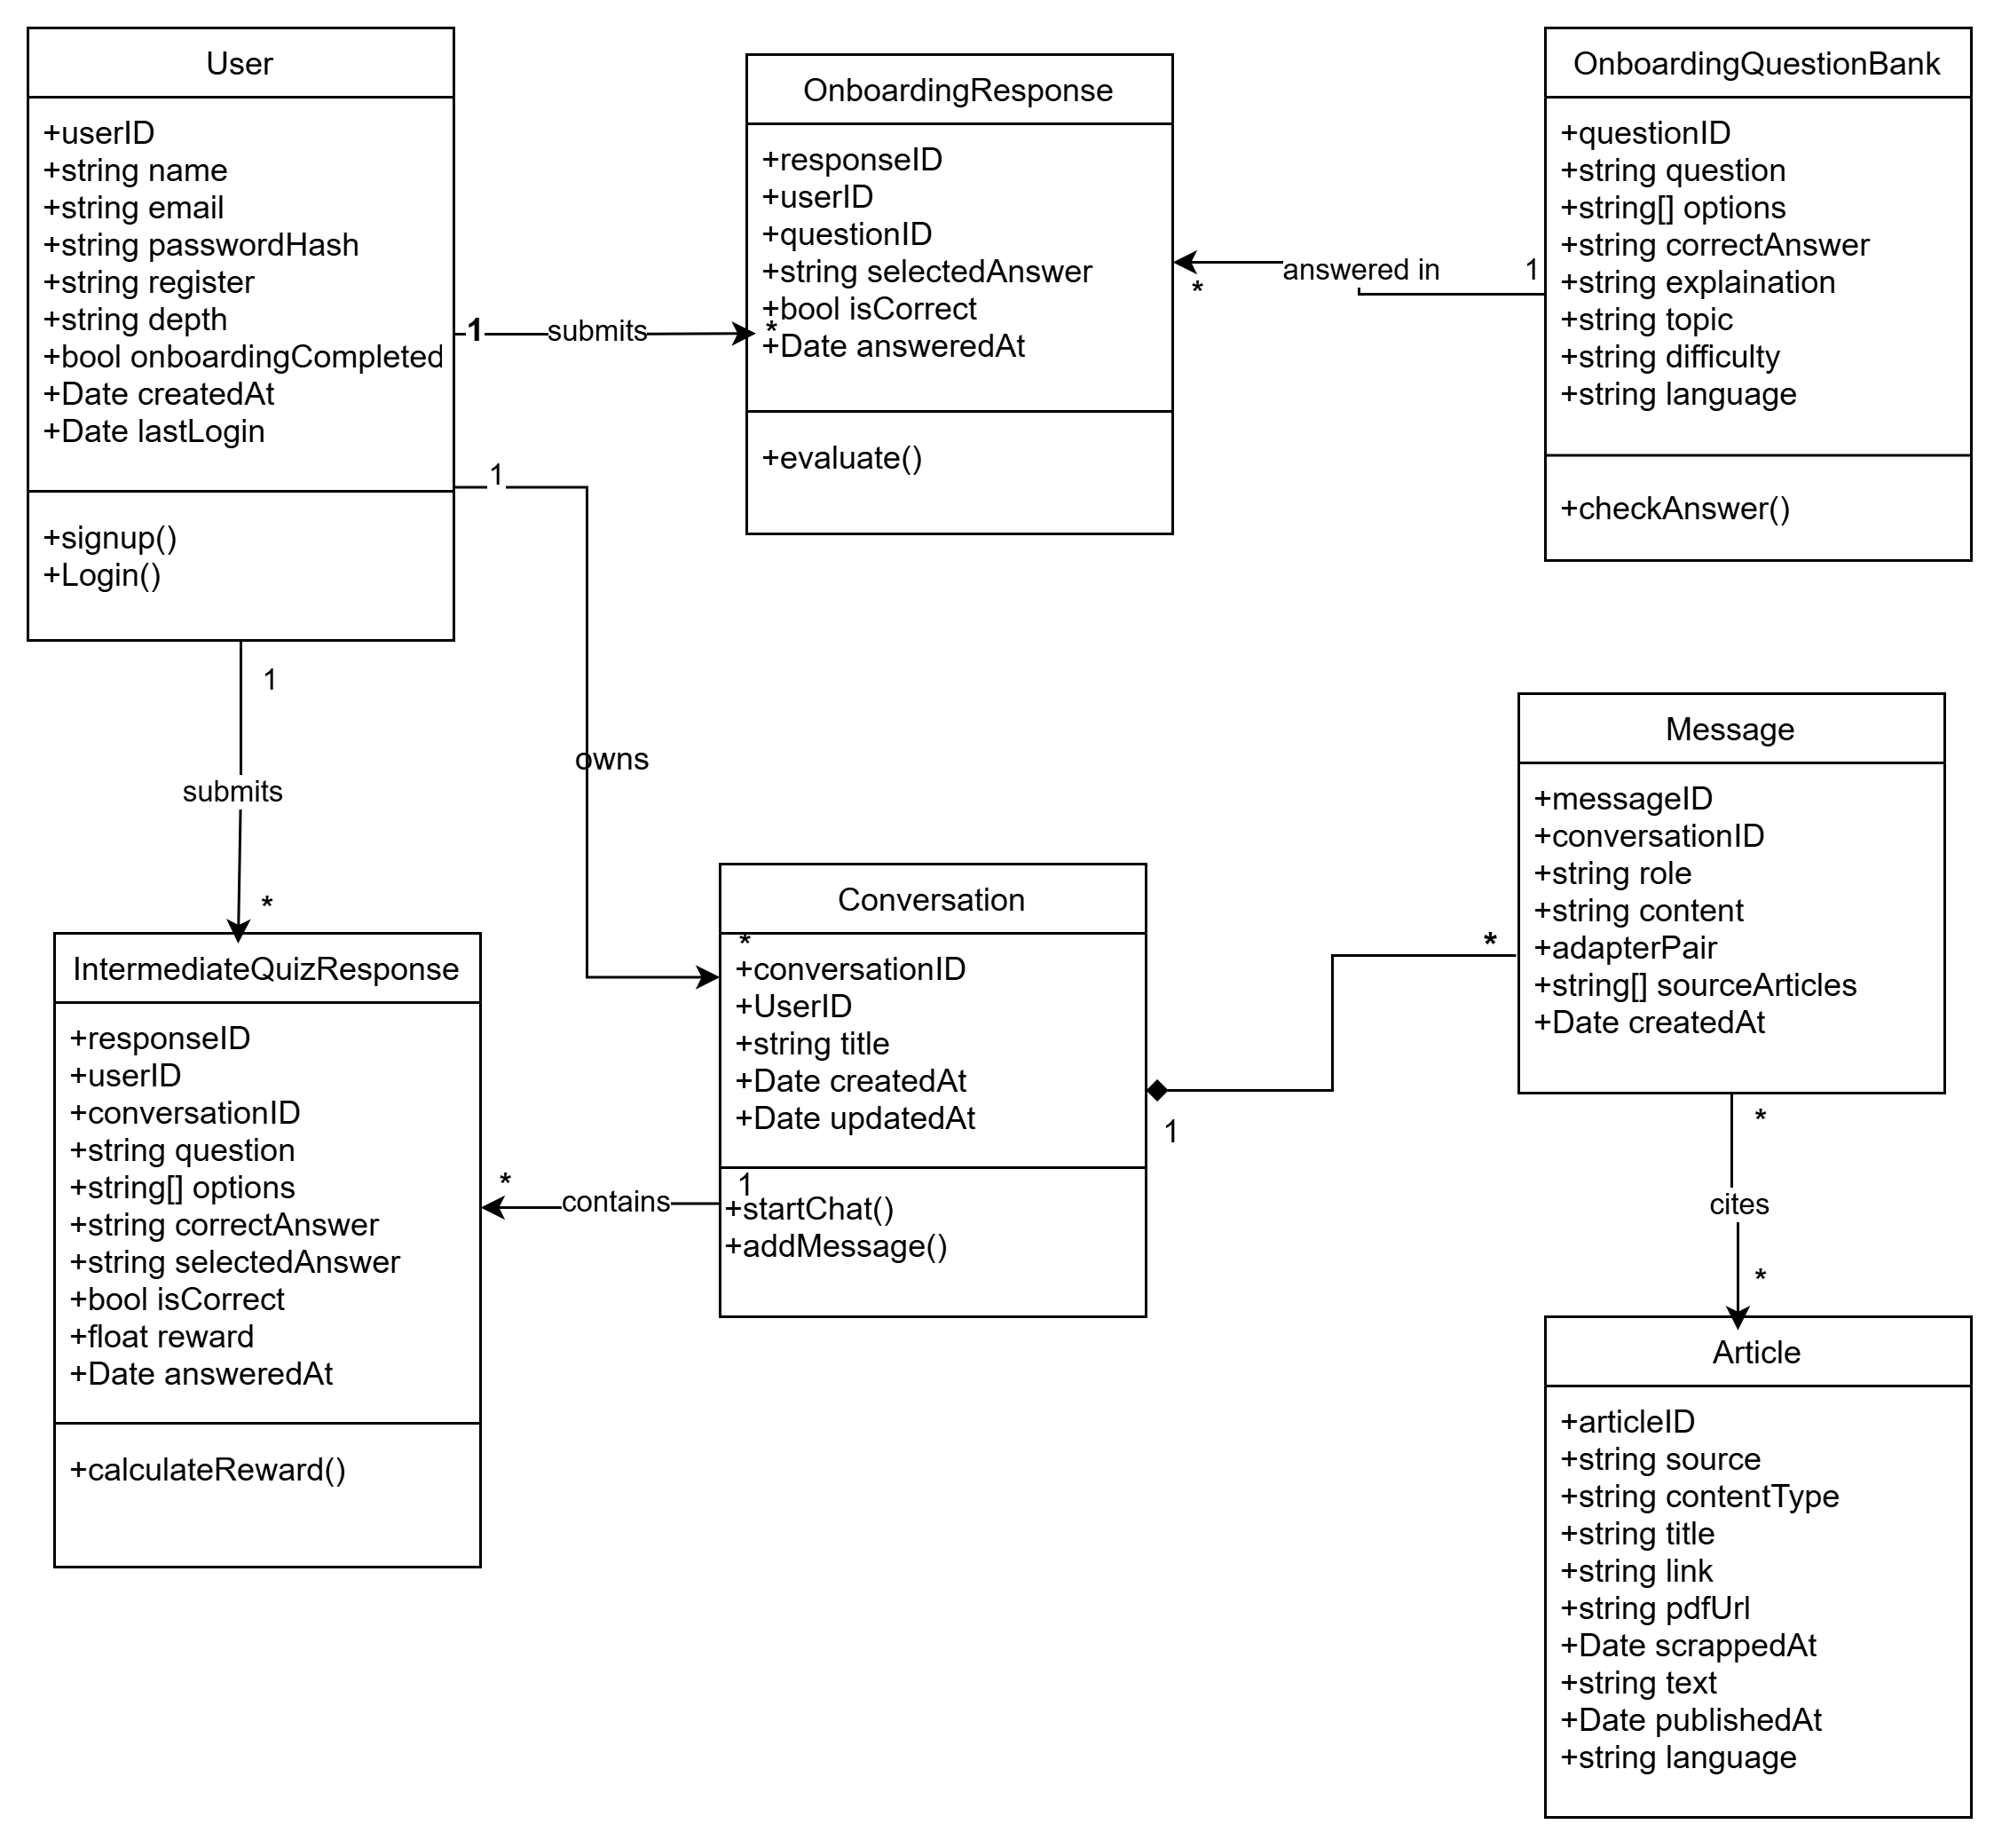
\includegraphics[width=0.85\textwidth]{Figures/classdiagram.png}
    \caption{Class diagram}
    \label{fig:classdiagram}
\end{figure}

\section{Sequence Diagrams}
\label{sec:sequence-diagrams}
A sequence diagram is a type of UML (Unified Modeling Language) diagram that shows how the parts of a system interact over time to carry out a task. Each participant is drawn as a lifeline, messages between participants are drawn as arrows in the order they occur, and activation bars show when a participant is busy handling a request. Solid arrows represent requests and dashed arrows represent responses, while framed regions mark alternative paths (\textit{alt}), optional steps (\textit{opt}), repeated steps (\textit{loop}) and early exits (\textit{break}). The learner is the only actor in DiploMind, so the following figures cover every flow that a learner starts, from registration and onboarding to asking questions, taking quizzes and managing chats.

\begin{figure}[H]
    \centering
    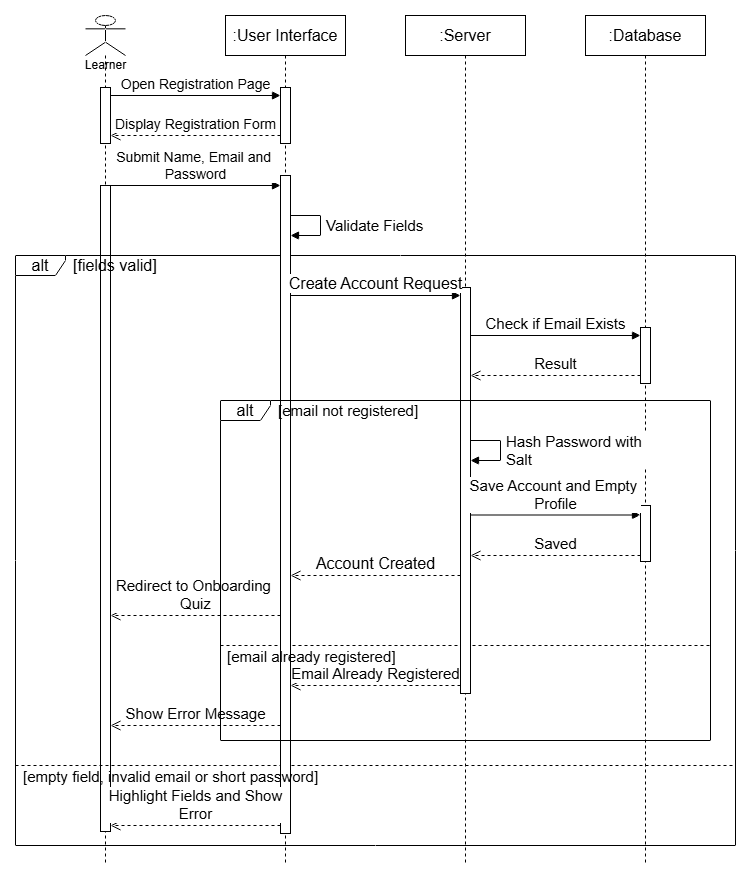
\includegraphics[width=\textwidth, height=0.8\textheight, keepaspectratio]{Figures/SD_1.png}
    \caption{Sequence of User Registration}
    \label{fig:sd-registration}
    \vspace{2pt}
    \textit{Flow/Sequence of operations followed by the system when a new learner creates an account.}
\end{figure}

\begin{figure}[H]
    \centering
    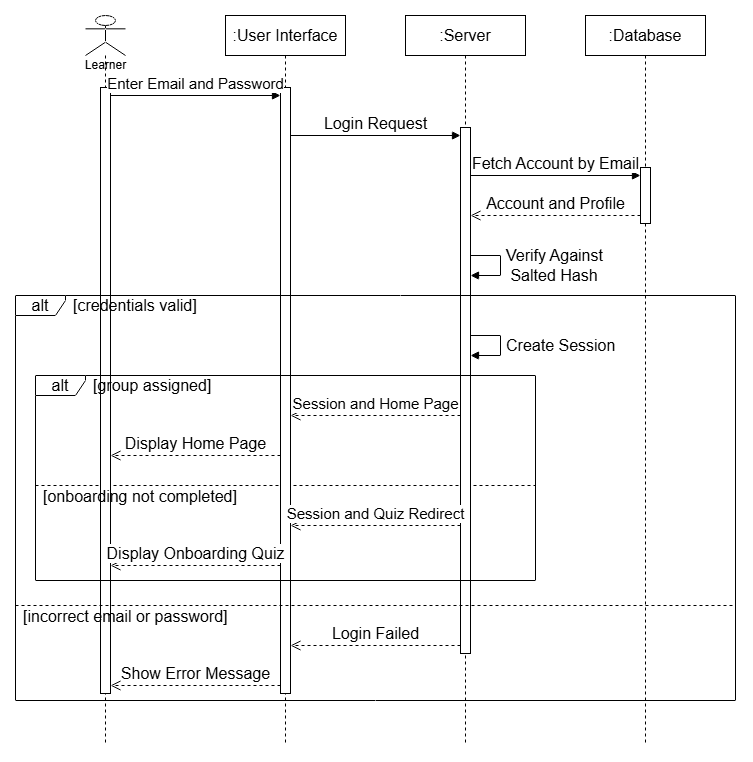
\includegraphics[width=\textwidth, height=0.8\textheight, keepaspectratio]{Figures/SD_2.png}
    \caption{Sequence of User Login}
    \label{fig:sd-login}
    \vspace{2pt}
    \textit{Flow/Sequence of operations followed by the system when a learner signs in, including redirection to the onboarding quiz.}
\end{figure}

\begin{figure}[H]
    \centering
    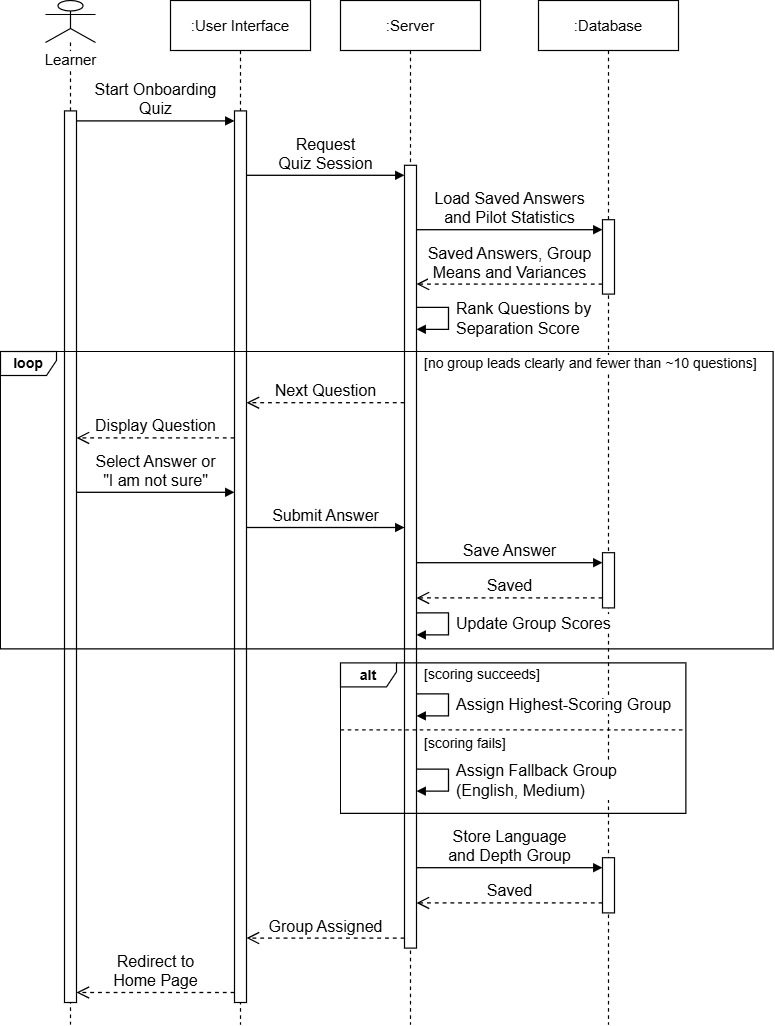
\includegraphics[width=\textwidth, height=0.8\textheight, keepaspectratio]{Figures/SD_3.png}
    \caption{Sequence of Onboarding Quiz}
    \label{fig:sd-onboarding}
    \vspace{2pt}
    \textit{Flow/Sequence of operations followed by the system to place a new learner into one of the nine language and depth groups.}
\end{figure}

\begin{figure}[H]
    \centering
    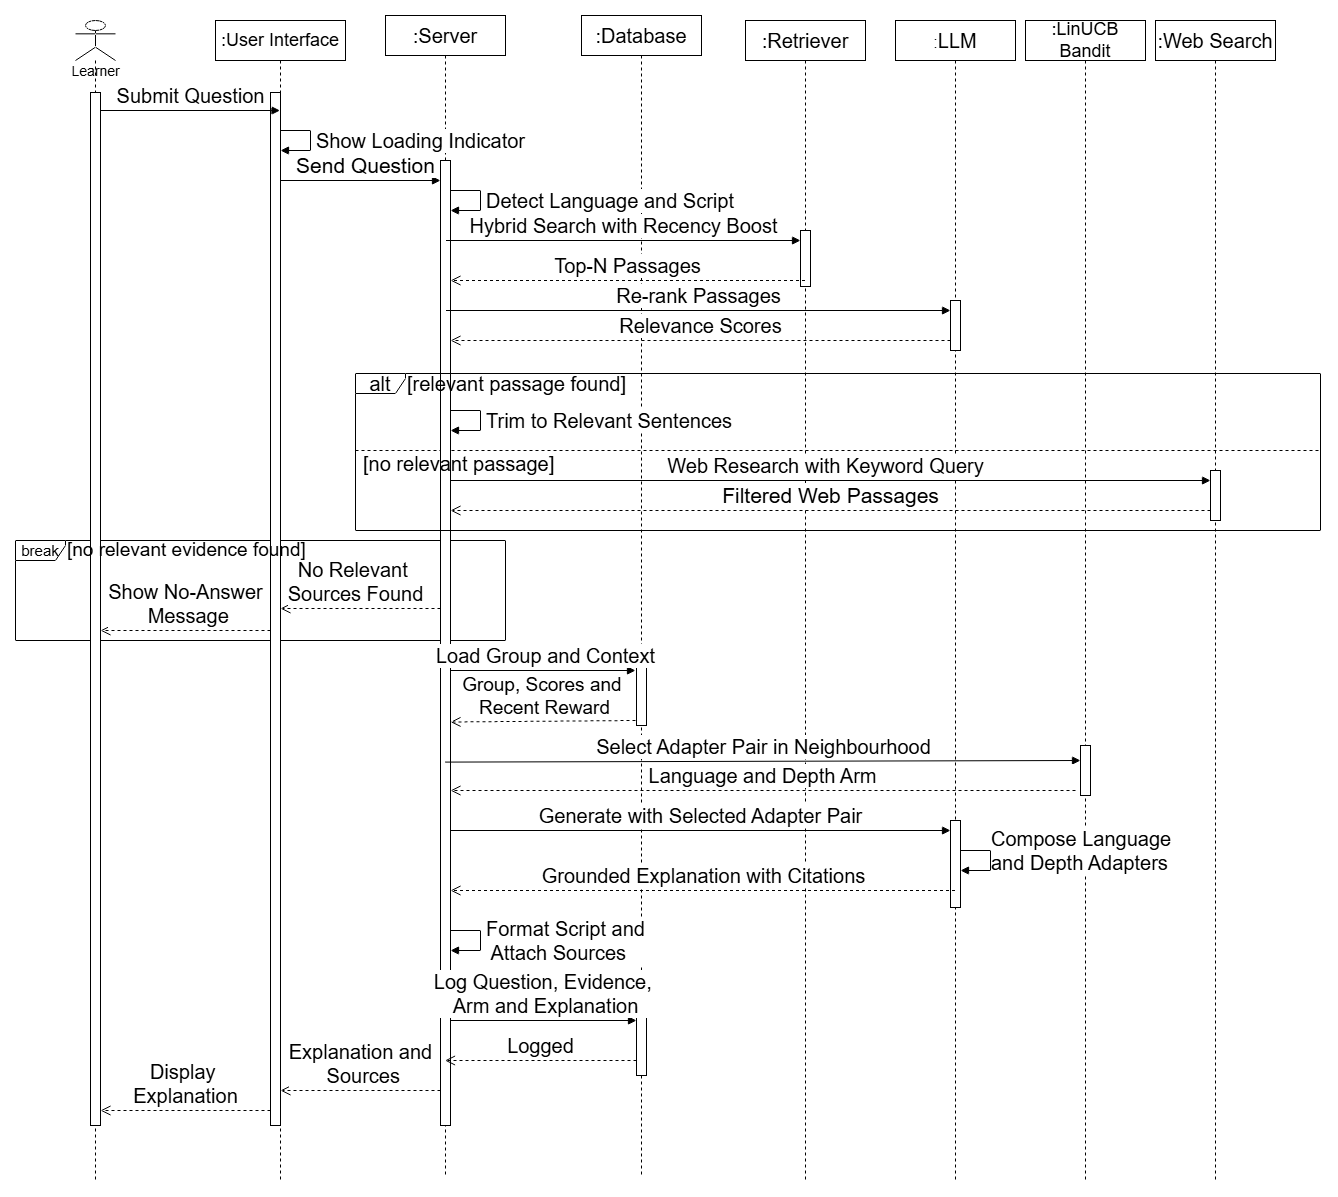
\includegraphics[width=\textwidth, height=0.8\textheight, keepaspectratio]{Figures/SD_4.png}
    \caption{Sequence of Asking a Question}
    \label{fig:sd-question}
    \vspace{2pt}
    \textit{Flow/Sequence of operations followed by the system to retrieve evidence, select an adapter pair and generate a personalized explanation.}
\end{figure}


\begin{figure}[H]
    \centering
    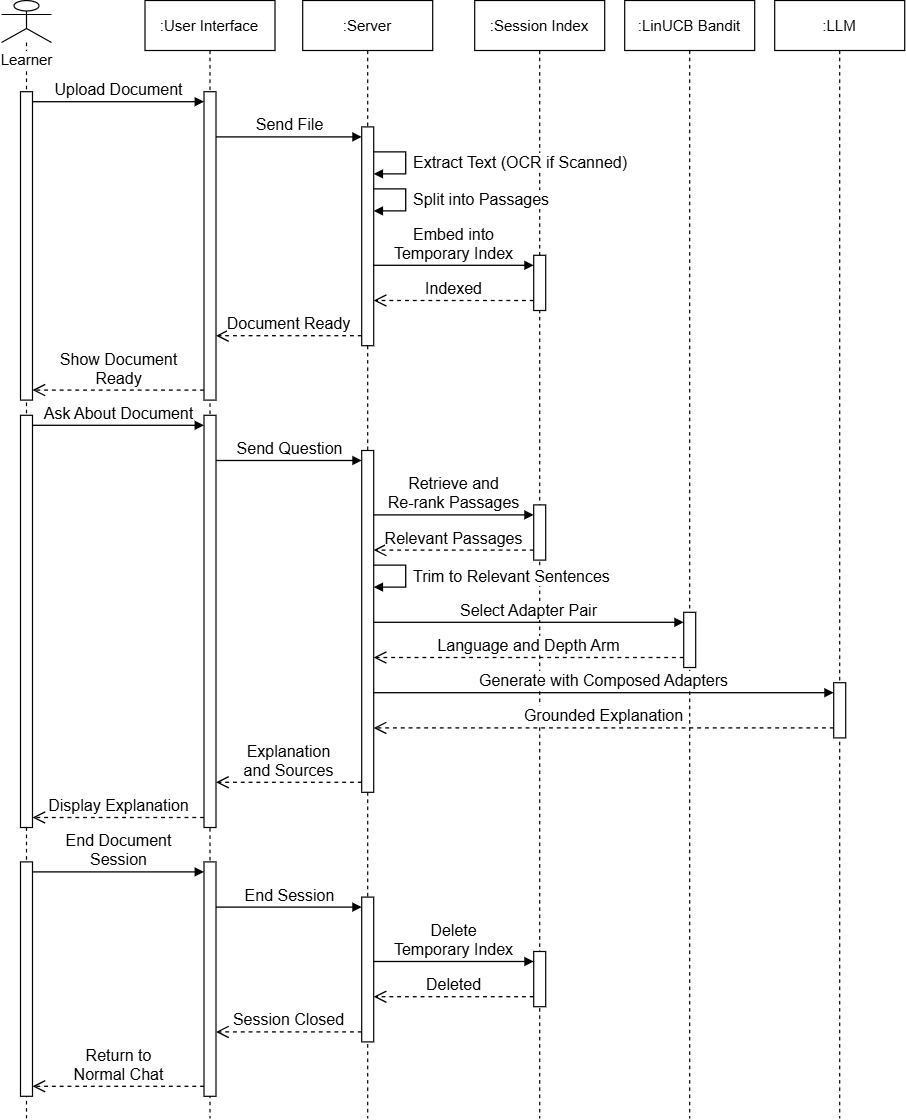
\includegraphics[width=\textwidth, height=0.8\textheight, keepaspectratio]{Figures/SD_5.png}
    \caption{Sequence of Document Upload}
    \label{fig:sd-document}
    \vspace{2pt}
    \textit{Flow/Sequence of operations followed by the system to explain a learner's uploaded document through a temporary session index.}
\end{figure}

\section{Policies and Tactics}
The following are the policies and tactics that will be followed in the project, along with the alternatives that were considered.

\subsection{Coding Guidelines and Code Organization}
The project is written mainly in Python, so we will follow the PEP~8 standard for naming, formatting and code layout, and document every module and public function with docstrings. The code will be split into separate packages for scraping, retrieval, adapters, the bandit, the drift monitor and the API, so that each part can be developed and tested on its own and new features can be added without changing the others. Tunable values such as the composition weights, the exploration parameter and the drift thresholds will be kept in configuration files instead of being hard-coded, and random seeds will be fixed in experiments so that results can be reproduced.

\subsection{Choice of Database}
We will use a NoSQL document database for learner profiles, chats, interaction logs and quiz results. These records are nested and vary in shape, for example an interaction holds its retrieved passages, citations and the adapter pair used, and the logged fields are likely to change as the reward and bandit features are finalized. A relational database was considered, but it would need frequent schema changes during development and several joins to rebuild a single chat. The relations in DiploMind are simple (a learner has chats, and a chat has interactions), so the weaker join support of a document database is an acceptable trade-off.

\subsection{Choice of Algorithms}
LinUCB was chosen for adapter selection because it explores according to its uncertainty instead of at random, which gave better results than $\epsilon$-greedy exploration when data were scarce \cite{li2010contextual}, and DiploMind will start with few learners. For personalization, six adapters are combined by weighted addition instead of training nine joint adapters, which would need more training data and a new adapter for every added language or depth. Personalization through the prompt alone was rejected, since earlier work found that prompting cannot reliably combine several preferences \cite{jang2023personalized}. If our ablation shows that composition does not preserve both language and depth, jointly trained adapters will be used as a fallback. For onboarding, the adaptive question selection of Shams et al. \cite{shams2021cluster} is preferred, with fixed-threshold scoring kept as a simpler alternative.

\subsection{Safe Exploration and Reassignment}
The bandit may only choose the learner's current adapter pair or a neighbouring pair (one depth step up or down, or another language at the same depth), and its exploration parameter is kept small at first. Unrestricted exploration was rejected because it could show a technical explanation to a beginner simply as an experiment. Reassignment follows the same caution: a learner is moved only when a neighbouring group is expected to do better by a set margin, and a cool-down period after each move prevents the learner from being switched back and forth.

\subsection{Grounding and Source Policy}
Every explanation will be generated only from retrieved passages and will show its sources. If no relevant passage is found in the knowledge base or through the web research fallback, the learner is told so instead of receiving an unsupported answer. Answering from the model's own knowledge was rejected because international relations content is political and current, and an unsupported or outdated claim could mislead the learner. When the web fallback is used, reliable news and analysis sources are preferred over unknown websites.

\subsection{Data Handling and Privacy}
Passwords will be stored only as salted hashes, and each learner can access only their own profile, chats and quiz results. Documents uploaded by a learner are kept in a temporary index for that session and deleted afterwards, and are never added to the shared knowledge base. Logs used to improve the adapters will not contain names or email addresses. Scraped articles are used for research only and are not redistributed, and paywalled content is excluded.

\subsection{User Interface}
The interface will be simple and consistent, so that learners without a technical or IR background can use it without instructions. Urdu text will be shown right-to-left in a readable Urdu font, Urdish in Roman script and English left-to-right. Every explanation will list its sources, a loading indicator will be shown while an answer is generated, and every onboarding question will offer an ``I am not sure'' option so that learners are not forced to guess.

\subsection{Testing}
Unit tests will cover the onboarding scoring, the bandit updates, the reward calculation and the drift rules. Integration tests will check the full question pipeline, from retrieval to the formatted answer, and black-box tests will follow each use case, including its alternative flows. Because there are few real users at the start, the bandit and the drift monitor will be tested with simulated learners, some of them deliberately placed in the wrong group. Urdu and Urdish outputs will be reviewed by native speakers, and adapters will be evaluated on a fixed held-out test set before each demonstration.

\subsection{Engineering Trade-offs}
Several trade-offs shape the implementation. A 7--8B base model loaded in 4-bit precision fits on a 16~GB GPU but gives somewhat lower quality than a larger model. Re-ranking passages with an LLM improves the evidence used for an answer but adds to the response time. Quizzing after every 5--10 prompts gives the bandit a regular reward signal, while quizzing more often would tire the learner. Roman script for Urdish was rated more natural by native speakers \cite{winata2026codeswitched}, but it has no standard spelling, which makes evaluation harder. For the slow improvement loop, we will start with reward-filtered fine-tuning, the simplest option, and move to preference optimization or GRPO only if time allows.

\section{Conclusion}
This chapter presented the design of DiploMind. It gave an overview of the system and its five modules, and described the assumptions, dependencies, constraints, and guidelines that shaped the design. The architecture was divided into an offline preparation part and an online learning part, with a subsystem view of each module. The architectural strategies explained the choice of one shared base model with six adapters, retrieval-augmented generation, a client-server model, and a NoSQL database alongside a vector database. Sequence diagrams showed the main learner flows, and the policies and tactics recorded the choices made on algorithms, safe exploration, grounding, privacy, and testing, along with the alternatives that were rejected. Together, these decisions keep explanations grounded in sources, personalization safe for the learner, and each component replaceable, and they provide the basis for implementation.


\chapter{Implementation and Test Cases}
For each chapter, provide a paragraph of introduction and at the end, a paragraph of conclusions. (Not the programming code but the algorithmic and procedural details especially related to the hidden/ backend algorithms that are not covered in the design)
\section{Implementation}
Whatever implementation that you have done so far, please elaborate here.
Give clear details of the algorithms that were implemented along with the platform and the APIs which were used. 
\textcolor{red}{NOTE: For FYP-1, this chapter can be changed to description of prototype developed.}
\subsection{Implementation of First Component/Algorithm}
Write the implementation of the first component of your system here.

\begin{comment}
\section{Test case Design and description}
\textcolor{red}{This section will be added in FYP-II.} Summarize the common attributes of test cases. This may include input constraints that must be true for every input in the set of associated test cases, any shared environmental needs, any shared special procedural requirements, and any shared case dependencies. The following scheme is recommended for describing test cases in detail. The Sample test case is provided in table \ref{tab:3}.
\begin{table}[!ht]
\caption{Sample Test case No.1}

\centering
\begin{tabular}{|llll|}
\hline
\multicolumn{4}{|c|}{\textbf{\textless{}Software Component Name\textgreater{}}} \\ \hline
\multicolumn{4}{|c|}{\textbf{\textless{}Reference\textgreater{}}} \\ \hline
\multicolumn{1}{|l|}{\textbf{Test Case ID:}} &
  \multicolumn{1}{l|}{\textit{Reference Number}} &
  \multicolumn{1}{l|}{\textbf{QA Test Engineer:}} &
  \textit{Name of personnel} \\ \hline
\multicolumn{1}{|l|}{\textbf{Test case Version:}} &
  \multicolumn{1}{l|}{\textit{Version number}} &
  \multicolumn{1}{l|}{\textbf{Reviewed By:}} &
  \textit{Testing Team lead} \\ \hline
\multicolumn{1}{|l|}{\textbf{Test Date:}} &
  \multicolumn{1}{l|}{\textit{Date}} &
  \multicolumn{1}{l|}{\textbf{\begin{tabular}[c]{@{}l@{}}Use Case \\ Reference(s):\end{tabular}}} &
  \textit{Relation to use cases} \\ \hline
\multicolumn{1}{|l|}{\textbf{Revision History:}} &
  \multicolumn{3}{l|}{\textit{Refer to previous test   case identity (if any)}} \\ \hline
\multicolumn{1}{|l|}{\textbf{Objective:}} &
  \multicolumn{3}{l|}{\textit{Need and   scope of the testing}} \\ \hline
\multicolumn{1}{|l|}{\textbf{\begin{tabular}[c]{@{}l@{}}Product/Ver/\\ Module:\end{tabular}}} &
  \multicolumn{3}{l|}{\textit{Refer to overall system being built and the place of this test case in it.}} \\ \hline
\multicolumn{1}{|l|}{\textbf{Environment:}} &
  \multicolumn{3}{l|}{\textit{Necessary and desired properties of the test environment.}} \\ \hline
\multicolumn{1}{|l|}{\textbf{Assumptions:}} &
  \multicolumn{3}{l|}{\textit{Assumptions that might affect the testing process.}} \\ \hline
\multicolumn{1}{|l|}{\textbf{Pre-Requisite:}} &
  \multicolumn{3}{l|}{\textit{Necessary condition that  needs to be fulfilled before the test case.}} \\ \hline
\multicolumn{1}{|l|}{\textbf{Step No.}} &
  \multicolumn{1}{l|}{\textbf{Execution   description}} &
  \multicolumn{2}{l|}{\textbf{Procedure result}} \\ \hline
\multicolumn{1}{|l|}{} &
  \multicolumn{1}{l|}{\textit{Events being tested.}} &
  \multicolumn{2}{l|}{\textit{Mention software response.}} \\ \hline
\multicolumn{4}{|l|}{\textbf{Comments:}} \\ \hline
\multicolumn{4}{|c|}{\textbf{Passed      Failed     Not Executed}} \\ \hline
\end{tabular}
\label{tab:3}
\end{table}
\section{Test Metrics}
Summarize here the common ground of attributes of test case metrics as explained in Table \ref{tab:4}.
\begin{table}[!ht]
\centering
\caption{Sample Test case Matric.No.1}

\begin{tabular}{|l|l|}
\hline
\textbf{Metric}                      & \textbf{Purpose}                                                                                                        \\ \hline
\textbf{Number of Test Cases}        & \begin{tabular}[c]{@{}l@{}}Total number of test cases that you have\\ developed for  your system.\end{tabular}          \\ \hline
\textbf{Number of Test Cases Passed} & The number of test cases that successfully passed                                                                       \\ \hline
\textbf{Number of Test Cases Failed} & The number of test cases that failed                                                                                    \\ \hline
\textbf{Test Case Defect Density}    & \begin{tabular}[c]{@{}l@{}}(No of test cases failed * 100) \\ No of test cases executed\end{tabular}                    \\ \hline
\textbf{Test Case Effectiveness}     & \begin{tabular}[c]{@{}l@{}}No of defects detected using test cases *100\\ Total number of defects detected\end{tabular} \\ \hline
\textbf{Traceability Matrix} &
  \begin{tabular}[c]{@{}l@{}}Traceability is the ability to determine that each\\  the feature has a source in requirements and each \\ requirement has a corresponding implemented feature.\end{tabular} \\ \hline
\end{tabular}
\label{tab:4}
\end{table}
\subsection{Sample Test case Metric.No.2}
Similar to the above table, add here for test metrics 2,3,4.\\
\chapter{User Manual}
\textcolor{red}{This chapter will be added in FYP-II.} Design a complete user manual of your application and add that in this chapter.
\textcolor{red}{NOTE: This Chapter is optional for Research projects but compulsory for Development projects.}\\ 
\end{comment}

\providecommand{\ph}[1]{\textbf{[#1]}}
\providecommand{\phfig}[2]{\fbox{\parbox[c][#1][c]{0.88\textwidth}{\centering\textit{#2}}}}
\chapter{Experimental Results and Discussion}
This chapter reports the experimentation involving the base Model selection along with the training and evaluation of the six LoRA adapters of Diplomind i.e. three language adapters (Urdu, Urdish, English) and three depth adapters (easy, medium, technical). The base model selection involved running 4 candidate models on the same samples and then reviewing the quality of them using automated language following checks as well as human reviews. Each adapter was trained on its own training set and evaluated against the base model on a fixed test set. The cahapter describes the experimental setup and the evaluation metrics, presents the model selection findings, training behaviour and test results of each adapter and discusses what the results show and where they are limited.

\section{Experimentation Overview}
The experiments had two parts. The first compared four candidate models without any fine-tuning, in order to choose the base model on which all adapters would be trained (Section~\ref{sec:base-selection}). The second tested whether a small LoRA adapter can reliably teach that frozen base model one controllable property of its output, either the language (and script) of an explanation or its depth. Five questions guided the experiments.
 
\begin{itemize}
    \item Which of the four candidate models already handles Urdu and Urdish best, without any fine-tuning?
    \item Does each adapter lower the loss of the base model on unseen articles?
    \item Does the adapted model follow the requested language or depth more consistently than the base model?
    \item Does the adapter keep the output faithful to the source article (names, numbers and facts unchanged)?
    \item How do the six adapters compare with each other in training behaviour and final quality?
\end{itemize}
 
The base-model comparison selected Llama 3.1 8B Instruct, and all six adapters were trained on it. Every adapter was trained with the same recipe so that differences between adapters come from their training data and not from their settings. All adapter results are measured on the same held-out test articles. The base-model comparison was run before any training and used its own small set of test inputs, which is described in Section~\ref{sec:base-selection}.
 
\begin{comment}
\chapter{Conclusions}
\section{aa}
\subsection{dfs}
\subsubsection{dsd}
{\bf This chapter is mandatory}.  
Give conclusions and summary of the work done.  What were your findings and what were the results?  Discuss in detail whether the scope of your project was entirely covered or not and whether the objectives of the project were met or not.  What challenges did you face and what has been left out and why.\\
Sum up all the conclusions of all the chapters here to make a final conclusion chapter.  Do not repeat any text, just summarize it in different words. Give recommendations for future work also.\\
\textbf{For FYP-1 it is mandatory to list down a plan of the work to be done for FYP-2.}
\end{comment}

{
\bibliographystyle{ieeetr}
\bibliography{fypbib} %specify your .bib file here
}
%ADD APPENDICES IF REQUIRED OTHERWISE COMMENT IT OUT
\begin{comment} % 1. Load the package
\appendix
\chapter{First Appendix if Required}
If you want to add appendices then make sure you provide a proper title.  Add different appendices by using the chapter command as shown for this one.  They will automatically be added to the table of contents.

\section{References}
See how .bib file is prepared.  The bibliography would be automatically added by Latex.  So here is how you cite papers (you'll need to view the .bib file to understand).  \cite{ref:Duda:2000} is the correct way to make one citation and \cite{ref:Bishop:2006,ref:SVMGuide} to make multiple citations. You can see various reference styles for manuals \cite{ref:SVMGuide}, conferences \cite{ref:guyon:2007}, websites \cite{ref:IJCNNChallenge:2007} and journal articles \cite{ref:guyon:2007a}.  Also, note that all citations appear in the order in which they appear within text.  They are not sorted according to author names.

\section{Equations}
Make sure you use the math environment for writing equations.  Again, make sure you do not hard code equation numbers.  Use label and ref commands of Latex to number them and reference them.  Here is an example of (\ref{eq:energy})
\begin{equation}\label{eq:energy}
E = mc^2
\end{equation}
Note, how the equation is referenced by its equation number within brackets.  

\section{Figures}
To insert a figure, you can use the following code as template.  Here the figure is referenced using ref command of Latex.  So Figure \ref{fig:fast} is the FAST logo.  DO NOT HARD CODE FIGURE NUMBERS.  Let Latex manage them for you.

\begin{figure}[!hbt]
\centering

\includegraphics[width=1in]{Figures/fastlogo.png}
{\caption {\label{fig:fast}{\textbf{Fast Logo is the Caption.}}}}  
\end{figure}

\section{Tables}
Note how tables can be added in Latex.  Also, make sure you use label and ref commands to define and use table numbers.  You can use Table \ref{tbl:SomeTable} as a template to make tables, add captions to them and reference them.  DO NOT HARD CODE TABLE NUMBERS.  Let Latex manage their numbering for you.

If you are having problems in managing Latex tables, you may use Lyx \url{https://www.lyx.org/}. 


\begin{table}[hbt]

\begin{center}
\caption{\label{tbl:SomeTable} \textbf{Give a Caption to the Table.}}
\begin{tabular}{|l|c|c|} 
\hline
\textbf{No.}&\textbf{Column 1}&\textbf{Column 2}\\
\hline
1.&Some data&More data\\
\hline
2.&Some values&More values\\
\hline
\end {tabular}

\end{center}

\end{table}

\section{Pseudo Code}
When you need to explain an existing algorithm of an algorithm you devised, then you should use pseudo code notation. Given below, algorithm  \ref{algo:one}, is an example. Note how the numbering is managed by the Latex itself.

\begin{algorithm}[H]
 \KwData{this text}
 \KwResult{how to write algorithm with \LaTeX2e }
 initialization\;
 \While{not at end of this document}{
  read current\;
  \eIf{understand}{
   go to next section\;
   current section becomes this one\;
   }{
   go back to the beginning of current section\;
  }
 }
 \caption{How to write algorithms}
 \label{algo:one}
\end{algorithm}

\section{Code of Programming Languages}
If you need to add C++, Java or any other programming language's code, then you can use ``listings'' package. Following is an example. Normally, the code is only added in the appendices to avoid clutter in the document.

\begin{lstlisting}

#include <stdio.h>
#define N 10
/* Block
 * comment */

int main()
{
    int i;

    // Line comment.
    puts("Hello world!");
    
    for (i = 0; i < N; i++)
    {
        puts("LaTeX is also great for programmers!");
    }

    return 0;
}
\end{lstlisting}

\section{Recommendations for \LaTeX}
Here we are providing you with only two Latex source files.  main.tex and fypbib.bib file. You can also start a project at \url{overleaf.com} and upload the zip file of this template there and share the Latex source between your group and supervisor.  This way all of you can work on the Latex files together online.
\end{comment}

\end{document}


